\documentclass[10pt, conference, letterpaper]{IEEEtran}
\usepackage{epstopdf}
\usepackage{amssymb, graphicx}
\usepackage{cite}
\usepackage{url}
\usepackage{amsmath}
\usepackage{color}
\usepackage[normalem]{ulem}
\usepackage{multirow}
\usepackage{epsfig}
\usepackage{subfigure}
\usepackage{comment}
\usepackage{balance}
\usepackage[T1]{fontenc}


%\makeatother
%
%\usepackage{float}
%% \usepackage{pifont}
%% \usepackage[small]{caption}
%\usepackage[it]{caption}
%\usepackage{amsmath,epsfig,amssymb}
%\usepackage{graphicx}
%\usepackage{subfigure}
%\usepackage{wrapfig}
%\usepackage[table]{xcolor}
%\usepackage{multirow}
%\usepackage{algorithmic}
%\usepackage{algorithm}
%\usepackage{mathrsfs}
%\usepackage{array}
%\usepackage[table]{xcolor}
%\def\pdfshellescape{1}
%\usepackage{epstopdf}
%\usepackage{auto-pst-pdf}
%\usepackage{url}
%\usepackage{makecell}% \usepackage{appendix}
%\usepackage{lipsum}
%
%\usepackage{marvosym} % happy face packages
%
%\setcounter{MaxMatrixCols}{40}
%
%\newcommand{\qed}{\hfill \mbox{\raggedright \rule{0.05in}{0.05in}}}
%\newtheorem{theorem}{Theorem}
%\newtheorem{lemma}{Lemma}
%\newtheorem{proposition}{Proposition}
%\newtheorem{corollary}{Corollary}
%\newtheorem{proof}{Proof}

%\makeatother
%
%\usepackage{float}
%\usepackage{pifont}
%\usepackage[small,it]{caption}
%\usepackage{amsmath,epsfig,amssymb}
%\usepackage{graphicx}
%\usepackage{subfigure}
%\usepackage{wrapfig}
%\usepackage[table]{xcolor}
%\usepackage{multirow}
%\usepackage{algorithmic}
%\usepackage{algorithm}
%\usepackage{mathrsfs}
%\usepackage{array}
%\usepackage[table]{xcolor}
%\def\pdfshellescape{1}
%\usepackage{epstopdf}
%\usepackage{auto-pst-pdf}
%\usepackage{url}
%\usepackage{makecell}
%
%\definecolor{Gray}{gray}{0.9}
%\newcolumntype{g}{>{\columncolor{Gray}}c}

\begin{document}
\title{Software defined Network Inference with Passive/active Evolutionary-optimal pRobing (SNIPER)}

%
\maketitle
% gyl0511@gmail.com wangxiong@uestc.edu.cn

\begin{abstract}
A key requirement for network management is accurate and reliable network monitoring where critical information about internal characteristics or states of the network(s) must be obtained. In today's large-scale networks, this is a challenging task due to the hard constraints of network measurement resources. In this paper, a new framework (called SNIPER) is proposed where we use the flexibility provided by Software-Defined Networking (SDN) to design the optimal observation or measurement matrix which leads to the best achievable estimation accuracy using Matrix Completion (MC) techniques. Here, to cope with the inherent complexity of the process of designing large-scale optimal observation matrices, we use the well known Evolutionary Optimization Algorithms (EOA) which directly target the ultimate estimation accuracy as the optimization objective function. We evaluate the performance of SNIPER using both synthetic and real network measurement traces from different network topologies and by considering two main applications including network traffic and delay estimations. Our results show that SNIPER is a flexible and efficient framework that can be used for a variety of network performance measurements under hard constraints of network measurement resources. For example, by measuring 8.8\% of per-flow path delays in Harvard network, congested paths can be detected by probability 0.94. To demonstrate the feasibility and effectiveness of our framework, we have implemented a prototype of SNIPER in Mininet.
\end{abstract}
%%% % \input{SNIPER14_KeyWords}
%%% % \section{Introduction}  \label{sec:SNIPERIntro}
%MC needs independent measurement --> no feasible aggregability issues
%hard resource constraint
%mention to direct measurement and their problems 
%change intro and add related works section
In computer networks, network management refers to the activities, methods, procedures, and tools that pertain to the operation, administration, maintenance, provisioning and security of networked systems \cite{Clemmi:2006}. To meet the QoS agreements, a key requirement for network management is accurate and reliable network monitoring where critical information about internal characteristics or states of the network(s) must be directly measured or indirectly inferred. In today's complex networks, the direct measurement of network's Internal Attributes of Interest (IAI) can be challenging or even inefficient and infeasible due to the hard constraints of network measurement resources including the limited number of Ternary Content Addressable Memory (TCAM) entries at switches, the limited processing power and storage capacity and limited available bandwidth in active network performance measurement. Network Inference (NI) techniques are powerful network monitoring tools that can help estimate the IAI based on a limited set of measurements. Therefore, NI problems are naturally ill-posed in the sense that the number of measurements are not sufficient to uniquely and accurately determine the solution. Hence, side information from different perspectives and sources must be incorporated into the problem formulation to improve the estimation precision \cite{QZhao:2006} \cite{MDFE:2013} \cite{HNguyen:2007}. % \cite{Medina} \cite{Cao:2000} \cite{Roughan:2012}

Recently, Matrix Completion (MC) techniques have been used as network inference tools where the problem is the completion of a matrix of IAI from the direct measurement of a sub-set of its entries \cite{Roughan:2012}\cite{Gursun:2011}\cite{YLiao:2011}. Since in communication networks a variety of resources of the communication infrastructure at different layers are shared, the main assumption in MC techniques is that the matrix of IAI is a low-rank matrix which contains spatio-temporal redundancies and thus not all of its entries are needed to represent it; accordingly missed or non-observed entries can be estimated from a sub-set of randomly measured entries. In the theory of matrix completion, the matrix of IAI can be completely reconstructed from a sub-set of observed/measured entries (indicating the observation/measurement matrix) if the number of \emph{randomly} chosen observations are \emph{high} enough \cite{Candes:2009}\cite{Candes:2010}. Accordingly, in \cite{Roughan:2012} and \cite{Gursun:2011} the MC methods are used for network Traffic Matrix (TM) completion to estimate the missed entries of the TMs. Also, in \cite{YLiao:2011}, a new MC technique has been used for active network performance measurements where the status of path delays or bandwidths are predicted from a set of active measurements and using a new MC technique.

%On the other hand, nowadays, Software-Defined Networking (SDN) offers the required flexibility and interfaces to effectively implement different network monitoring, management and control tasks. In fact, an SDN enabler, such as OpenFlow, nicely separates the measurement data plane and control plane functions, and provides a capability to control/re-program the internal configurations of switches in dynamic environments. Consequently, SDN allows for more complex network monitoring and management applications \cite{IF14iSTAMP:2014} \cite{YLiao:2011} \cite{MYu:2011} \cite{MYu:2013}. %  in an adaptive and efficient way

On the other hand, Software-Defined Networking (SDN), along with its OpenFlow enabler, is an emerging technology that nicely separates the measurement data plane and control plane functions, and provides a capability to control/re-program the internal configurations of switches in dynamic environments. Consequently, SDN allows to adaptively and efficiently implement more complex network monitoring applications, including both passive and active network measurements, without the need of customization. For passive network measurement, the most SDN based works related to traffic engineering and network security applications where the main goal is focused on network traffic measurement or identifying Heavy Hitters (HH) and Hierarchical Heavy Hitters (HHH). In \cite{MYu:2011} and \cite{MYu:2013}, reconfigurable measurement architectures are proposed where a variety of sketches for different measurement tasks can be defined and installed by the operator. In \cite{Tootoonchian:2010}, OpenTM estimates a traffic matrix by keeping track of statistics for each flow. Recently, in \cite{IF14iSTAMP:2014}, an intelligent SDN based traffic measurement framework (called iSTAMP) with the ability of adaptive and accurate fine-grained flow estimation is proposed. For active network measurement under SDN paradigm, the very recent work \cite{Adrichen:2014} establishes a general framework where accurate measurements of per-flow throughput, packet loss and delay can be measured.

Here, since matrix completion techniques use the independent measurements of IAI, without suffering from the problem of feasibility of providing aggregated side information (such as the method of optimal flow aggregation in \cite{IF14iSTAMP:2014}), we use the flexibility provided by the SDN to address the following interesting question:

\emph{Under hard resource constraints of network measurement resources, how can we optimally measure or sample a sub-set of entries of the matrix of IAI and design the optimal observation matrix which leads to the best possible estimation accuracy via using matrix completion techniques?}
% and accordingly does not suffer from the problem of the feasibility of optimal aggregation techniques as in \cite{IF14iSTAMP:2014} for 
%Accordingly, in network monitoring applications, matrix completion techniques along with the flexibility provided by the SDN can be used to address the following interesting question:\emph{
%Under hard resource constraints of network measurement resources, how can we optimally measure or sample a sub-set of entries of the matrix of IAI and design the optimal observation matrix which leads to the best possible estimation accuracy via using matrix completion techniques?}
%% Such an optimal measurement/observation matrix is efficient in the sense that it needs less number of measurements to reach the same estimation accuracy via random measurement scheme, or equivalently, for the same number of measurements the optimal sampling techniques reaches a better perfromance.

However, the \emph{direct} design of optimal observation matrices for maximizing the performance of NI methods is prohibitive due to the complexity of the process \cite{IF14iSTAMP:2014}\cite{Elad:2007}. To simplify this process, other objective functions (e.g. coherency \cite{Elad:2007} or condition number \cite{MDFE:2013}) are considered in the optimization process, while accepting the unavoidable sacrifice in the performance \cite{Elad:2007}. The underlying difficulty in this direct optimal observation matrix design is that formulating the network inference process or algorithm into a closed-form and well-defined mathematical objective function that can be efficiently optimized is extremely complicated and computationally complex, if it is not impossible or intractable. 

Therefore, in this paper, we propose a new approach in designing the optimal observation matrix for network inference problems where we \emph{directly} target the ultimate estimation accuracy in network monitoring applications in our optimization framework. However, to cope with the inherent complexity of the process of designing large-scale optimal observation matrices, we use the well known Evolutionary Optimization Algorithms (EOA) that are suitable for the optimization problems where the main objective function is a procedure or an algorithm that can not be formulated as a well-defined mathematical function. In this framework, the evolutionary optimization algorithm acts as a \emph{sniper} which precisely captures or measures the best entries of the matrix of IAI which leads to the best estimation accuracy via matrix completion techniques. 
% The SNIPER framework is built upon the recent achievements in the theory of matrix completion to develop a practical foundation for the design of optimal measurement or observation matrices under hard resource constraints of network measurement resources.
%\subsection{Related Works}
%The flexibility provided by SDN and its enabler OpenFlow has been used to implement most of the passive and active network monitoring tasks in different applications without the need of customization. For passive network measurement, the most SDN based works related to traffic engineering and network security applications where the main goal is focused on network traffic measurement or identifying aspects of the network traffic such the presence of Heavy Hitters and Hierarchical heavy hitters. In \cite{MYu:2011}, the authors propose a reconfigurable measurement architecture for hierarchical heavy hitter detection, and then, \cite{MYu:2013} they propose a re-programmable structure (called OpenSketch) where a variety of sketches for different measurement tasks can be defined and installed by the operator. In \cite{Tootoonchian:2010}, OpenTM estimates a traffic matrix by keeping track of statistics for each flow. Recently, in \cite{IF14iSTAMP:2014} we have proposed an intelligent SDN based traffic measurement framework (called iSTAMP) with the ability of adaptive and accurate fine-grained flow estimation. For active network measurement under SDN paradigm, the very recent work \cite{Adrichen:2014} establishes a general framework where accurate measurements of flow throughput, packet loss and delay can be obtained.
%% \subsection{Our contributions}
%Under hard constraints of measurement resources in network monitoring applications, the SNIPER is a simple, generic, and efficient framework with the ability to optimally measure the most informative IAI which lead to the best achievable estimation accuracy via matrix completion methods. In fact, SNIPER can be easily deployed on commodity OpenFlow-enabled routers/switches to enhance the performance of various passive or active network monitoring applications with low computation and communication overhead between control and data planes. Here, we build upon the recent achievements in the theory of matrix completion to develop a practical foundation for guiding
%the design of optimal measurement or observation matrices under hard resource constraints of network measurement resources. 

Under hard constraints of measurement resources in network monitoring applications, the SNIPER is a simple, generic, and efficient framework which can be easily deployed on commodity OpenFlow-enabled routers/switches to enhance the performance of various passive or active network monitoring applications with low computation and communication overhead between control and data planes. Since MC techniques are the main NI methods in SNIPER, which directly use partial independent measurements of IAI, thus, this framework not only can be easily implemented in a centralized manner but also it can be implemented in distributed or decentralized ways. Accordingly, it is compatible with the recent trends in developing more smart and agile SDN platforms \cite{Bianchi:2014}\cite{Moshref:2014} where data plane APIs and switches are able to execute codes inside the device with no further interaction with the controller. Accordingly, our main contributions are summarized as follow:

\textbf{$\text{\hspace{0.1cm}}\bullet$} To the best of our knowledge for the first time, we use the EOAs to design the optimal observation matrix where ultimate network inference performance is the main objective function to be optimized, where we show that under hard constraint of measurement resources the optimal design of the observation matrix provides more accurate estimates.

\textbf{$\text{\hspace{0.1cm}}\bullet$} We address the scalability, deployability and feasibility of the SNIPER: a) by reducing the computational complexity of EOAs; b) by introducing a new online learning algorithm which concurrently measures and learns and c) by evaluating the performance of our framework using both synthetic and real network measurement traces from different network topologies in two main applications including network traffic and delay estimation, and further, by implementing a prototype of SNIPER in Mininet environment.

The rest of this paper is organized as follows. Section~\ref{sec:SNIPERSysDsc} provides an overview of SNIPER and
the matrix completion techniques that we have used as our main NI methods.  In Section~\ref{sec:SNIPEREvlObsMtxDsg} we describes our
optimal observation matrix design procedure using the EOAs. Then, in Section~\ref{sec:SNIPERPerfEvalApp}, we explain our methodology for evaluating the performance of the SNIPER. Accordingly, in Section~\ref{sec:SNIPERPerfEvalApp} we evaluate the performance of SNIPER considering two main applications including per-flow path delay and per-flow size estimations. Section~\ref{sec:Conclu} summarizes our most important results. 

%connect to resources allocation strategies (active learning)
\section{Introduction}  \label{sec:SNIPERIntro}
The direct measurement of network's Internal Attributes of Interest
(IAI) such as the Origin-Destination Flow (ODF) sizes (as a measure of
traffic intensity between nodes) or per-flow delay, throughput or
packet loss, can be challenging or even inefficient and infeasible due to
scale, complexity and limited availability of network measurement
resources. In large-scale networks, the measurement resources,
including the Ternary Content Addressable Memory (TCAM) entries,
processing power, storage capacity and available bandwidth,
are very limited, and hence, rendering per-flow direct measurements are
infeasible. To cope with scalability issues, Network Inference (NI)
techniques can be leveraged to estimate various IAI based on partial
passive and/or active measurements. However, NI problems are naturally
ill-posed in the sense that the number of measurements are not
sufficient to uniquely and accurately determine the solution. Hence,
side (supplementary) information from different sources and perspectives must be incorporated into the problem formulation to improve
the estimation precision \cite{QZhao:2006} \cite{MDFE:2013}
\cite{HNguyen:2007}.

Software-Defined Networking (SDN) provides data plane and control
plane separation enabling capability to dynamically control and
re-program network switches. Most current researches have focused on
leveraging SDN flexibility to implement complex network management and control
applications, such as, route control \cite{SDXGupta:2014}\cite{Rothenberg:2012}. However, SDN can also enable adaptive
and efficient implementation of passive and active network monitoring
applications that can be controlled dynamically at run-time
\cite{MYu:2011} \cite{MYu:2013} \cite{IF14iSTAMP:2014}
\cite{Adrichen:2014}. This is of particular importance in many network
management and security applications where accurate and reliable
network monitoring is necessary to provide critical information about
internal characteristics or states of the network(s) that must be
directly measured or indirectly inferred.
% \cite{Medina} \cite{Cao:2000} \cite{Roughan:2012}

Network inference techniques can
utilize the run-time programmability provided by the SDN to optimize
and facilitate the process of collecting the required direct
measurements and/or side information. In fact, the capabilities of SDN
have been utilized in a variety of passive and active network
monitoring applications. Most SDN based passive measurement studies
are related to traffic engineering and network security applications,
such as, network traffic measurement or identifying Heavy Hitters (HH)
and Hierarchical Heavy Hitters (HHH). In \cite{MYu:2011} and
\cite{MYu:2013}, SDN reconfigurable measurement architectures are
proposed where a variety of sketches for different direct measurement
tasks can be defined and installed by the operator. In
\cite{Tootoonchian:2010}, OpenTM directly measures a traffic matrix by
keeping track of statistics for each flow. Recently, in
\cite{IF14iSTAMP:2014}, an intelligent SDN based traffic measurement
framework (called iSTAMP) with the ability of adaptive and accurate
fine-grained flow estimation is proposed. For active network
measurement under SDN paradigm, the very recent work
\cite{Adrichen:2014} establishes a general framework (called
Opennetmon) where accurate measurements of per-flow throughput, packet
loss and delay can be directly measured.

% here for \cite{MYu:2013} IAI is a binary vector which represents the sate of measurements and inference is the HH detection technique (will be added to this paragraph)
However, the state of the art SDN-enabled traffic measurement and
inference methods, for example in \cite{MYu:2013}
\cite{IF14iSTAMP:2014}, suffer from the following challenges. First,
these frameworks are not generally applicable and are mainly limited
to network traffic size measurement. Second, the longest prefix matching
forwarding in OpenFlow implies that incoming flows can be aggregated
in just one entry of the TCAM, and hence, the capability of providing
optimal redundant aggregated measurements is limited. Thus, constructing required optimal aggregated measurements are not always feasible; this is known as \emph{feasibility} constraint, here. Third, in
\cite{IF14iSTAMP:2014}, to simplify the process of designing the
optimal aggregation (i.e. measurement) matrix, the ultimate estimation
accuracy is not directly targeted. Instead, the coherency of the
measurement matrix is minimized, leading to unavoidable sacrifice in
the performance \cite{IF14iSTAMP:2014}\cite{Elad:2007}.
% Third, in \cite{IF14iSTAMP:2014}, the main objective function in the design of optimal aggregation matrix does not target the main estimation accuracy and, therefore, it accepts the unavoidable sacrifice in the performance.

On the other hand, recently, Matrix Completion (MC) techniques have
been used as powerful network inference tools that involve completing
a matrix of IAI from the direct measurement of a sub-set of its
independent entries
\cite{Roughan:2012}\cite{Gursun:2011}\cite{YLiao:2011}. Examples of
the matrix of IAI include a matrix where each entry is an ODF at
different times \cite{Roughan:2012}, or per-flow delay/packet-loss
between different nodes of the network \cite{YLiao:2011}. Since a
variety of resources and information are often shared across different
layers in communication networks, the main assumption in MC techniques
is that the matrix of IAI is a low-rank matrix which contains
spatio-temporal redundancies, and thus, not all of its entries are
needed to represent it. Consequently, missed or non-observed entries can
be estimated from a sub-set of randomly measured entries \cite{Candes:2009}. In the
theory of matrix completion, the matrix of IAI can be completely
reconstructed from a sub-set of observed/measured entries (indicating
the observation/measurement matrix) if the number of \emph{randomly}
chosen observations is \emph{high} enough
\cite{Candes:2009}\cite{Candes:2010}. Therefore, in
\cite{Roughan:2012} and \cite{Gursun:2011} the MC methods are used for
network Traffic Matrix (TM) completion to estimate the missed entries
of the TMs. Also, in \cite{YLiao:2011}, a new MC technique is used for active network performance measurements where the status of path delays or bandwidths are predicted from a set of active
measurements.

In this paper we propose a novel approach to combine SDN
programmability with MC techniques for reconstructing the matrix of
IAI from a sub-set of directly measured \emph{independent}
entries. Thus paving the way for: 1) designing an efficient framework
for different passive/active network measurement applications under
hard constraint of measurement resources, and 2) providing required
side information without feasibility constraints (as in
\cite{IF14iSTAMP:2014}). For this purpose, we define an observation matrix for the direct measurements of IAI that can be used by different matrix completion techniques and we answer the following interesting question:

\emph{Given limited network measurement resources, how we can use the SDN capabilities to directly measure a sub-set of entries of the IAI matrix and thus design the Optimal Observation Matrix (OOM) leading to the best possible estimation accuracy using matrix completion techniques?}

However, the \emph{direct} design of OOM for
maximizing the performance of NI methods is prohibitive due to the
complexity of the process \cite{IF14iSTAMP:2014}\cite{Elad:2007}. The
underlying difficulty lies in the fact that formulating the network
inference process or algorithm, as a function of the observation
matrix which targets the ultimate estimation accuracy, into a
closed-form and well-defined optimization problem that can be
efficiently optimized is extremely complicated and computationally
complex, if it is not impossible or intractable. 

Therefore, in this
paper, we propose a new approach in designing the optimal observation
matrix for network inference problems where we \emph{directly} target
the ultimate estimation accuracy of network monitoring applications in
our optimization framework. However, to cope with the inherent
complexity of the process of designing large-scale OOM, we use the well-known Evolutionary Optimization Algorithms
(EOA) that are suitable for the optimization problems where the main
objective function is a procedure or an algorithm that can not be
formulated as a well-defined mathematical function. In this framework,
the evolutionary optimization algorithm acts as a \emph{sniper} which
precisely measures the best or the most informative
entries of the matrix of IAI which leads to the best estimation
accuracy using matrix completion techniques. 

We refer to our proposed framework as Software defined Network Inference with Passive/active Evolutionary-optimal pRobing (SNIPER). The SNIPER is a simple, flexible, and efficient framework that utilizes MC technique to estimate all IAI using partial direct measurements. This framework can be easily deployed on commodity OpenFlow-enabled routers/switches in a centralized or distributed manner. Accordingly, it is
compatible with the recent trends in developing more smart and agile
SDN platforms \cite{Bianchi:2014}\cite{Moshref:2014} where data plane
APIs and switches are able to execute codes inside the device with no
further interaction with the controller. 

Our main contributions are summarized as follows:

\textbf{$\text{\hspace{0.1cm}}\bullet$} To the best of our knowledge, this is the first time that EOAs are applied to design the OOM where ultimate network inference performance is the main objective function to be optimized. We show that under hard constraint of measurement resources the optimal design of the observation matrix provides more accurate estimates of IAI, including per-flow size and delay. Moreover, the status of IAI can be reliably identified with sufficient precision in different network monitoring applications. For example, by measuring 8.8\% of per-flow path delays in Harvard network, congested paths can be detected by probability 0.94. This framework has also low communication and computation overheads.
%\textbf{$\text{\hspace{0.1cm}}\bullet$} To the best of our knowledge,
%this is the first time that EOAs are applied to design the OOM where ultimate network inference performance is the
%main objective function to be optimized. We show that under hard
%constraint of measurement resources the optimal design of the
%observation matrix provides more accurate estimates in different
%network monitoring applications, including per-flow size and delay
%estimations. Our proposed framework has also low communication and computation overheads. 

\textbf{$\text{\hspace{0.1cm}}\bullet$} We address the scalability,
deployability and feasibility of the SNIPER framework: a) by reducing
the computational complexity of EOAs; b) by introducing a new adaptive
algorithm for network measurement in dynamic environments, and c) by
evaluating the performance of our framework using both synthetic and
real network measurement traces from different network topologies. We
applied SNIPER to two main applications: network traffic and delay
estimations. In addition, we have implemented a prototype of SNIPER in
Mininet.

The rest of this paper is organized as
follows. Section~\ref{sec:SNIPERSysDsc} provides an overview of the
SNIPER framework and the matrix completion techniques that we have
used as our main NI methods.  In Section~\ref{sec:SNIPEREvlObsMtxDsg},
we describe our optimal observation matrix design procedure using EOAs. Then, in Section~\ref{sec:SNIPERPerfEvalApp}, we explain our
methodology for evaluating the performance of the SNIPER. In
Section~\ref{sec:SNIPERResults}, we evaluate the performance of SNIPER
considering two main applications including per-flow delay and
per-flow size estimations. Section~\ref{sec:Conclu} summarizes our
most important results.
% \section{Introduction}  \label{sec:SNIPERIntro} 

The direct measurement of network's Internal Attributes of Interest
(IAI) such as the Origin-Destination Flow (ODF) sizes (as a measure of
traffic intensity between nodes) or per-flow delay, throughput or
packet loss, can be challenging or even inefficient and infeasible due
scale, complexity and limited availability of network measurement
resources. In large-scale networks, the measurement resources,
including the Ternary Content Addressable Memory (TCAM) entries,
processing power, storage capacity and limited available bandwidth,
are very limited, and hence, rendering per-flow measurements are
infeasible. To cope with scalability issues, Network Inference (NI)
techniques can be leveraged to estimate various IAI based on partial
passive and/or active measurements. However, NI problems are naturally
ill-posed in the sense that the number of measurements are not
sufficient to uniquely and accurately determine the solution. Hence,
side (supplementary) information from different sources and vantage
points must be incorporated into the problem formulation to improve
the estimation precision \cite{QZhao:2006} \cite{MDFE:2013}
\cite{HNguyen:2007}.

Software-Defined Networking (SDN) provides data plane and control
plane separation enabling capability to dynamically control and
re-program network switches. Most current research has focused on
leveraging SDN flexibility to implement complex network control
applications like route control. However, SDN can also enable adaptive
and efficient implementation of passive and active network monitoring
applications that can be controlled dynamically at run-time
\cite{MYu:2011} \cite{MYu:2013} \cite{IF14iSTAMP:2014}
\cite{Adrichen:2014}. This is of particular importance in many network
management and security applications where accurate and reliable
network monitoring is necessary to provide critical information about
internal characteristics or states of the network(s) that must be
directly measured or indirectly inferred.
% \cite{Medina} \cite{Cao:2000} \cite{Roughan:2012}

The network inference techniques to estimate a particular IAI can
utilize the run-time programmability provided by the SDN to optimize
and facilitate the process of collecting the required direct
measurements and/or side information. In fact, the capabilities of SDN
have been utilized in a variety of passive and active network
monitoring applications. Most SDN based passive measurement studies
are related to traffic engineering and network security applications,
such as, network traffic measurement or identifying Heavy Hitters (HH)
and Hierarchical Heavy Hitters (HHH). In \cite{MYu:2011} and
\cite{MYu:2013}, SDN reconfigurable measurement architectures are
proposed where a variety of sketches for different direct measurement
tasks can be defined and installed by the operator. In
\cite{Tootoonchian:2010}, OpenTM directly measures a traffic matrix by
keeping track of statistics for each flow. Recently, in
\cite{IF14iSTAMP:2014}, an intelligent SDN based traffic measurement
framework (called iSTAMP) with the ability of adaptive and accurate
fine-grained flow estimation is proposed. For active network
measurement under SDN paradigm, the very recent work
\cite{Adrichen:2014} establishes a general framework (called
Opennetmon) where accurate measurements of per-flow throughput, packet
loss and delay can be directly measured.

% here for \cite{MYu:2013} IAI is a binary vector which represents the sate of measurements and inference is the HH detection technique (will be added to this paragraph)
However, the state of the art SDN-enabled traffic measurement and
inference methods, for example in \cite{MYu:2013}
\cite{IF14iSTAMP:2014}, suffer from the following challenges. First,
these frameworks are not generally applicable and are mainly limited
to network traffic volume measurement. Second, the longest prefix matching
forwarding in OpenFlow implies that incoming flows can be aggregated
in just one entry of the TCAM, and hence, the capability of providing
optimal redundant aggregated measurements is limited. Third, in
\cite{IF14iSTAMP:2014}, to simplify the process of designing the
optimal aggregation (i.e. measurement) matrix, the ultimate estimation
accuracy is not directly targeted. Instead, the coherency of the
measurement matrix is minimized, leading to unavoidable sacrifice in
the performance \cite{IF14iSTAMP:2014}\cite{Elad:2007}.
% Third, in \cite{IF14iSTAMP:2014}, the main objective function in the design of optimal aggregation matrix does not target the main estimation accuracy and, therefore, it accepts the unavoidable sacrifice in the performance.

On the other hand, recently, Matrix Completion (MC) techniques have
been used as powerful network inference tools that involve completing
a matrix of IAI from the direct measurement of a sub-set of its
independent entries
\cite{Roughan:2012}\cite{Gursun:2011}\cite{YLiao:2011}. Examples of
the matrix of IAI include a matrix where each entry is an ODF at
different times \cite{Roughan:2012}, or per-flow delay/packet-loss
between different nodes of the network \cite{YLiao:2011}. Since a
variety of resources and information are often shared across different
layers in communication networks, the main assumption in MC techniques
is that the matrix of IAI is a low-rank matrix which contains
spatio-temporal redundancies, and thus, not all of its entries are
needed to represent it; accordingly missed or non-observed entries can
be estimated from a sub-set of randomly measured entries. In the
theory of matrix completion, the matrix of IAI can be completely
reconstructed from a sub-set of observed/measured entries (indicating
the observation/measurement matrix) if the number of \emph{randomly}
chosen observations are \emph{high} enough
\cite{Candes:2009}\cite{Candes:2010}. Accordingly, in
\cite{Roughan:2012} and \cite{Gursun:2011} the MC methods are used for
network Traffic Matrix (TM) completion to estimate the missed entries
of the TMs. Also, in \cite{YLiao:2011}, a new MC technique has been
used for active network performance measurements where the status of
path delays or bandwidths are predicted from a set of active
measurements and using a new MC technique.

In this paper we propose a novel approach to combine SDN
programmability with MC techniques for reconstructing the matrix of
IAI from a sub-set of directly measured \emph{independent}
entries. Thus paving the way for: 1) designing an efficient framework
for different passive/active network measurement applications under
hard constraint of measurement resources, and 2) providing required
side information without feasibility constraints (as in
\cite{IF14iSTAMP:2014}). Our approach uses different matrix completion
techniques as our main NI tools, and define an observation matrix for
SDN-enabled programmable direct measurements of IAI to be used by MC
algorithms. Specifically, we answer the following interesting
question:

\emph{Given limited network measurement resouces, how can we use the SDN capabilities to directly measure a sub-set of entries of the IAI matrix and thus design the optimal observation matrix leading to the best possible estimation accuracy using matrix completion techniques?}

However, the \emph{direct} design of optimal observation matrices for
maximizing the performance of NI methods is prohibitive due to the
complexity of the process \cite{IF14iSTAMP:2014}\cite{Elad:2007}. The
underlying difficulty lies in the fact that formulating the network
inference process or algorithm, as a function of the observation
matrix which targets the ultimate estimation accuracy, into a
closed-form and well-defined optimization problem that can be
efficiently optimized is extremely complicated and computationally
complex, if it is not impossible or intractable. Therefore, in this
paper, we propose a new approach in designing the optimal observation
matrix for network inference problems where we \emph{directly} target
the ultimate estimation accuracy in network monitoring applications in
our optimization framework. However, to cope with the inherent
complexity of the process of designing large-scale optimal observation
matrices, we use the well known Evolutionary Optimization Algorithms
(EOA) that are suitable for the optimization problems where the main
objective function is a procedure or an algorithm that can not be
formulated as a well-defined mathematical function. In this framework,
the evolutionary optimization algorithm acts as a \emph{sniper} which
precisely captures or measures the best or the most informative
entries of the matrix of IAI which leads to the best estimation
accuracy via using matrix completion techniques. We refer to our proposed framework as Software defined Network
Inference with Passive/active Evolutionary-optimal pRobing
(SNIPER). 

{\bf GOAL OF FOLLOWING PARAGRAPH IS NOT CLEAR.}
The SNIPER is a simple, flexible, and efficient framework
which can be easily deployed on commodity OpenFlow-enabled
routers/switches to enhance the performance of various passive or
active network monitoring applications with low computation and
communication overhead between control and data planes. Since MC
techniques (as the main NI methods employed by SNIPER) directly use
partial independent measurements of IAI, this framework can be easily
implemented in a centralized or distributed manner. Accordingly, it is
compatible with the recent trends in developing more smart and agile
SDN platforms \cite{Bianchi:2014}\cite{Moshref:2014} with data plane
APIs and switches are able to execute codes inside the device with no
further interaction with the controller.

Our main contributions are summarized as follows:

\textbf{$\text{\hspace{0.1cm}}\bullet$} To the best of our knowledge,
this is the first time that EOAs are applied to design the optimal
observation matrix where ultimate network inference performance is the
main objective function to be optimized. We show that under hard
constraint of measurement resources the optimal design of the
observation matrix provides more accurate estimates in different
network monitoring applications, including per-flow size and delay
estimations.

\textbf{$\text{\hspace{0.1cm}}\bullet$} We address the scalability,
deployability and feasibility of the SNIPER framework: a) by reducing
the computational complexity of EOAs; b) by introducing a new adaptive
algorithm for network measurement in dynamic environments, and c) by
evaluating the performance of our framework using both synthetic and
real network measurement traces from different network topologies. We
applied SNIPER to two main applications: network traffic and delay
estimations. In addition, we implemented a prototype of SNIPER in
Mininet.

The rest of this paper is organized as
follows. Section~\ref{sec:SNIPERSysDsc} provides an overview of the
SNIPER framework and the matrix completion techniques that we have
used as our main NI methods.  In Section~\ref{sec:SNIPEREvlObsMtxDsg}
we describes our optimal observation matrix design procedure using the
EOAs. Then, in Section~\ref{sec:SNIPERPerfEvalApp}, we explain our
methodology for evaluating the performance of the SNIPER. In
Section~\ref{sec:SNIPERResults}, we evaluate the performance of SNIPER
considering two main applications including per-flow path delay and
per-flow size estimations. Section~\ref{sec:Conclu} summarizes our
most important results.

% \section{SNIPER: System Description}  \label{sec:SNIPERSysDsc}
Figure \ref{fig:GBDSNIPER} shows the general block diagram of the SNIPER framework where the controller interacts with Software Defined Measurement Network (SDMN) via Network Measurement Controlling (NMC) messages to reconfigure the SDMN and poll the required measurements and statistics. The SDMN consists of a set of hosts and a sub-set of OpenFlow Switches (OFS) in the operating network, which guarantees all required IAI are \emph{observable} and \emph{measurable}, as it is our assumption here. The NMC messages include passive/active network measurement control messages that indicate which IAI must be accurately measured at different times and/or spaces and setup the SDMN, accordingly. In the SNIPER framework, the network measurement process is consisted of two stages, namely the learning and measurement epochs, as it is shown in Figure \ref{fig:EVSmpMC}. In the supervised learning stage and using a training data set, the optimal IAI that must be directly measured are precisely computed using an evolutionary optimization algorithm. Then, in the online measurement epoch, the SDN flexibility is used to reconfigure the SDMN and to collect the measurements of corresponding optimal IAI. By decreasing the dependency of the SNIPER framework on the initial training data set and adaptively updating the optimal observation matrix, this framework can also be deployed in dynamic environments.

%This framework can also be equipped with online EOAs where measurement and learning are concurrently performed without using the training data.
% \footnote{For optimal network monitor placement problem, please refer to \cite{LMa1:2014}, \cite{LMa2:2014} and \cite{XWang:2014}.}
%The SNIPER framework provides the ability of measuring a sub-set of the precisely chosen attributes of interest (called Optimal Network Probes (ONP)) of the operating network at different times and/or spaces which resulted in the best possible accuracy in estimating the set of all unknown attributes of interests.
\begin{figure}[t]
  \begin{center}
    {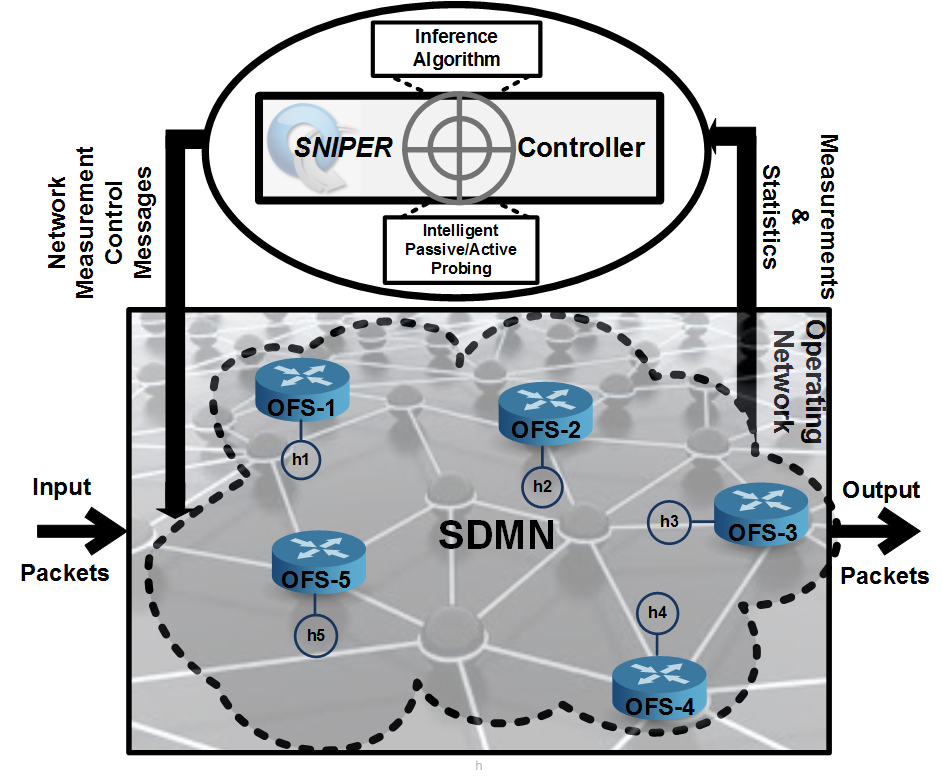
\includegraphics[keepaspectratio, width=0.49\textwidth]{GBDSNIPER_New.png}}
  \end{center}
  \caption{{SNIPER network measurement framework: a general perspective.}}
  \label{fig:GBDSNIPER}
\end{figure}
\begin{figure}[t]
  \begin{center}
    {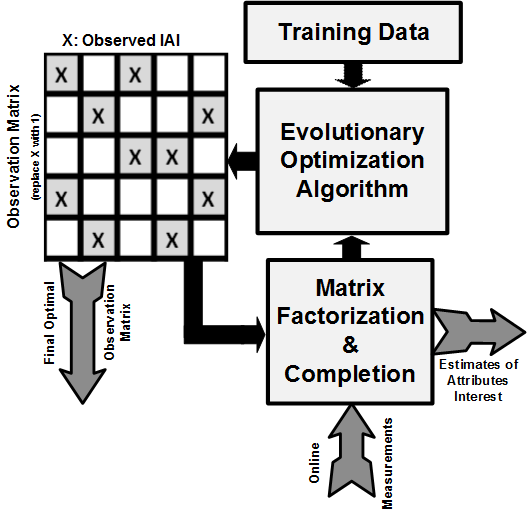
\includegraphics[keepaspectratio, width=0.35\textwidth]{EVSmpMC.png}} \\  % png
  \end{center}
  \caption{{Evolutionary optimal network probing process.}}
  \label{fig:EVSmpMC}
\end{figure}

% For passive measurement (e.g. per-flow size) the flow-tables of the SDMN is adaptively reconfigured. However, for active measurements (e.g. per-flow delay/loss) an appropriate path is first determined and flow-tables of the SDMN is adaptively reconfigured; then, probing packets are injected and routed, and required IAI are measured.
%The SNIPER controller can both preconfigure or adaptively reconfigure the flow-tables of the OFSs in SDMN. For passive per-flow size measurement, the flow-tables of the SDMN are configured and per-flow counter statistics are measured to form the matrix of per-flow sizes. In this case, ONMC messages (here, defined as passive probes) reconfigure the OFSs of the SDMN by installing different rules in flow tables and defining the required actions on the incoming packets of the operating network. 
The SNIPER controller can both preconfigure or adaptively reconfigure the flow-tables of the OFSs in SDMN. For passive per-flow size measurement, NMC messages (defined as passive probes, here) reconfigure the OFSs of the SDMN by installing different rules in flow tables and defining the required actions on the incoming packets. Accordingly, per-flow counter statistics are requested to measure and reconstruct the matrix of per-flow sizes. On the other hand, for active network performance measurements (e.g. per-flow delay/loss/throughput), appropriate paths are first determined (for all required entries of the matrix of IAI). Then, NMC messages are used to actively probe the operating network by: 1) adaptively configuring the flow-tables of the SDMN and their forwarding actions for probing packets sent by a set of hosts; 2) interacting with the injected probing packets into the network at the origin of the paths, and 3) collecting required measurements at destinations. Accordingly, the SNIPER can compute the required IAI and obtain information of active flows and monitor the end-to-end network performance measurements. These measurements are transmitted to the SNIPER controller where matrix completion techniques are used as the main NI algorithm to estimate all unknown IAI. In SNIPER, since MC techniques only need partial measurements, not only the communication overhead between switches and controller is low but also the amount of network resources used for passive per-flow size measurements (i.e. TCAM entries) and for active per-flow performance measurements (mainly bandwidth) are low.  

%The measurements are transmitted to the SNIPER controller where matrix completion techniques are used as the main NI algorithm to estimate all unknown IAI. The SNIPER controller can both preconfigure the switches with forwarding rules as well as it can reactively respond to requests from switches, which are sent when a packet matches none of the existing rules enters the network. Besides managing the forwarding plane, the SNIPER controller is also capable of requesting per-flow counter statistics and injecting packets into the network. Accordingly, the SNIPER architecture can obtain information of running flows and regularly injects packets into the network to monitor end-to-end network performance measurements \cite{IF14iSTAMP:2014}\cite{Adrichen:2014}. In this framework, the communication overhead between switches and controller is low, since MC techniques only needs partial measurements. 
% In fact, under the very hard constraints of measurement resources in network monitoring applications, this framework acts as a SNIPER which precisely captures/targets the ONPs. Accordingly, the IAI can be computed because communication networks share a variety of resources of the communication infrastructure (at different layers), and accordingly, there are spatial-temporal correlations/structures \cite{Roughan:2012}\cite{YLiao:2011}\cite{Gursun:2011} that can be used by the NI algorithm to improve the estimation accuracy in inferring IAI.

The feasibility of such Software-Defined Measurement (SDM) frameworks have been independently investigated in \cite{IF14iSTAMP:2014} and \cite{Adrichen:2014} where the capability of OpenFlow switches can be effectively utilized to measure and inference the IAI of the operating network. Likewise, the SNIPER controller is capable of providing: 1) per-flow sizes \cite{IF14iSTAMP:2014} by installing the flow ID prefixes in the flow tables and polls the statistics; 2) per-flow throughput \cite{Adrichen:2014} by determining specific path for each flow and queries switches to retrieve per-flow statistics where each query determines the amount of bytes sent and the duration of each flow; 3) per-flow packet loss \cite{Adrichen:2014} by polling flow statistics from the first and last switch of each path and subtracting the increase of the source switch packet counter with the increase of the packet counter of the destination switch, and 4) per-flow delay \cite{Adrichen:2014} by assigning a specific path to each flow and regularly injecting packets into the first switch and having the last switch send them back to the controller where the difference between the packet's departure and arrival times are computed by subtracting the estimated latency from the switch-to-controller delays. In this paper, the performance of the SNIPER framework is mainly examined in two main applications: per-flow size and delay estimations.
% For the details of the implementation please refer to \cite{IF14iSTAMP:2014} and \cite{Adrichen:2014}.
% In this paper, the performance of the SNIPER framework is mainly examined in two main applications including per-flow size and delay estimations using both synthetic and real network measurement traces from different network topologies. In addition, a prototype of SNIPER is implemented in the Mininet to demonstrate its implementation's feasibility and effectiveness.

\subsection{SNIPER: Problem Statement}   \label{subsec:ProbState}
The operating network is modeled as a connected undirected graph $G(V,E)$ where $|V|=N$, and $|E|=m$. Accordingly, there are $m$ links, and $n=N(N-1)$ paths and flows in the network, assuming that there exists an unique path between any pair of nodes in the network. As mentioned in the introduction, we model the NI problem as a Matrix Completion (MC) problem where the goal is to complete the matrix of attributes of interest ($X$) from the direct measurement of a sub-set of its entries assuming that $X$ is a low-rank matrix which contains redundancies and thus not all of its entries are needed to represent it. Here, $X$ is a matrix of size $n \times \mathcal{T}$ ($\mathcal{T}<n$) with rank $r << \mathcal{T}$ where $K$ entries of $X$ is directly measured. 
% The quantity $K$ is defined as $K=s.(n.\mathcal{T})$ where $s$ is the sampling ratio and $0 \leq s \leq 1$.
% In many network monitoring applications, the most important Internal Attributes of Interests (IAI) or performance metrics are flow size, flow throughput, packet loss and delay. Under hard resource constraints of network measurement resources (such as limited processing power and storage capacity, limited number of TCAM entries or limited bandwidth available in active loss/delay measurements) a Network Inference (NI) problem is defined as the process of estimating the IAIs based on a limited set of end-to-end or per-IAI's measurements.
% from just $O(n^{b} r log(n))$ \emph{randomly} observed entries, where $b$ is only slightly larger than 1. 

The theory of matrix completion \cite{Candes:2009} shows that under some suitable conditions, with high probability, $X$ can be exactly recovered from a set of sufficient \emph{randomly} observed entries. In practice, $X$ is often full rank but
with a rank $r$ dominant component, that is, $X$ has only $r$ significant singular values $\sigma_{1}$,..., $\sigma_{r}$ (where $\sigma_{1} \leq ... \leq \sigma_{r}$) and the others are negligible. In such cases, by minimizing the rank, a matrix of rank $r$ (denoted by $\hat{X}$) can still be found that approximates $X$ with high accuracy \cite{YLiao:2011}\cite{Candes:2009}\cite{Keshavan:2009}. Since direct minimization of the rank of a matrix is difficult, MC problems is often formulated as a convex optimization problem Eq.(\ref{MCFormu1}) where $\Omega$ is the set of observed (i.e. directly measured) entries, $P_{\Omega}$ is a sampling function that preserves entries of $X$ in $\Omega$ (i.e. $[P_{\Omega}(X)]_{ij}=x_{ij}$) and turns the others into zero, and, also $L$ is defined as $L(X,\hat{X}):=\sum_{i,j=1}^{n} (x_{ij}-\hat{x}_{ij})^{2}$. Corresponding to the sampling function $P_{\Omega}$, a Binary Observation Matrix $S_{\Omega}$ is also defined where $[S_{\Omega}(X)]_{ij}=1$. Accordingly, the MC searches for a low-rank matrix $\hat{X}$ that approximates $X$ with sufficient accuracy at the observed entries in $\Omega$. The unobserved or missing entries in $X$ (indicated by $\bar{\Omega}$ as the complement of $\Omega$) are predicted by the corresponding entries in $\hat{X}$. The MC problem can also be reformulated as a matrix factorization problem in Eq.(\ref{MCFormu2}) where $\hat{X}$ (with $rank(\hat{X}) \leq r$) is factorized as $\hat{X}=U_{n \times r}V_{r \times n}^{T}$ and $\lambda$ is the regularization coefficient that controls the extent of regularization. Here, the Frobenius norm of a matrix $Z$ is defined as $\left\|Z\right\|_{F}^{2}=\sum_{i,j=1}^{n} \left|z_{ij}\right|^{2}$. 

%Different methods can be used to solve optimization problem Eq.(\ref{MCFormu2}).
%The optimization problem Eq.(\ref{MCFormu2}) can be solved using different methods. 
\begin{equation}\label{MCFormu1}
%\small{
\begin{aligned}
\text{minimize} & \hspace{0.25cm} Trace \left( \hat{X} \right) = \sum_{i=1}^{n} \sigma_{i} \\
\text{s.t.} &  \hspace{0.25cm}  L\left(P_{\Omega}(X),P_{\Omega}(\hat{X})\right) \leq \delta
\end{aligned}
%}
\end{equation}

\begin{equation}\label{MCFormu2}
%\small{
\begin{aligned}
\underset{U,V}{\text{minimize}} & \hspace{0.25cm} L\left(P_{\Omega}(X),P_{\Omega}(\hat{X})\right) + \lambda ( \left\|U\right\|_{F}^{2} + \left\|V\right\|_{F}^{2} ) 
\end{aligned}
%}
\end{equation}

The optimization problem Eq.(\ref{MCFormu2}) can be solved using different methods. In this paper, we adopt two different methods from recently proposed MC procedures used in network monitoring applications to solve Eq.(\ref{MCFormu2}) and compute $U$ and $V$ matrices where $\hat{X}=UV^{T}$. The first one is the Sparsity Regularized Singular Value Decomposition (SRSVD) method \cite{Roughan:2012} that uses an alternating least squares procedure to solve Eq.(\ref{MCFormu2}). The second one is the Decentralized Matrix Factorization algorithm \cite{YLiao:2011},denoted by DMFSGD, that uses the Stochastic Gradient Descent (SGD) technique to solve Eq.(\ref{MCFormu2}). Both methods rely on the fact that the matrices of IAI in network monitoring applications contain temporal and/or spatial redundancies that can be used to estimate non-observed or missed entries.

Under hard resource constraints, it is crucial to design OOM, which leads to the best achievable estimation accuracy using matrix completion techniques. To show the importance of such a design, consider a 3$\times$3 matrix $X$ consisting of three spatial-independent processes in each row where $x_{1}(t)=\frac{1}{2}(x_{1}(t-1)+x_{1}(t+1))$, $x_{2}(t)=2x_{2}(t-1)+3$ and $x_{3}(t)=\frac{1}{2} x_{3}(t+1)-10$. Using the temporal structure in these processes, an OOM can be designed as $\Omega_{Opt}=[1, 0, 1; 1, 0, 0; 0, 0, 1]$ where there is at least one 1 in each row. Note that such an OOM can not guaranteed to be obtained using a random sampling strategy.

To maximize the performance of MC algorithms with minimum number of required measurements, such the process of designing the OOM must directly target the ultimate estimation accuracy in the network monitoring applications as defined in Eq.(\ref{NormMetrics}). However, it is extremely complicated, if it is not impossible, to formulate the MC process and target the ultimate performance criterion using a closed-form and well-defined mathematical optimization problem as a function of the observation matrix. In addition, since the observation matrix in our case is a binary matrix, it is computationally expensive and intractable to use integer optimization techniques in such a design process for large-scale networks. Therefore, in this paper, to cope with the inherent complexity of the process of designing large-scale optimal observation matrices, we apply well known evolutionary optimization algorithms that are suitable for optimization problems similar to ours.

%To maximize the performance of NI algorithms with minimum number of required measurements, such a design process must directly target the ultimate estimation accuracy in the network monitoring application. However, it is extremely complicated and computationally complex, if it is not impossible or intractable, to formulate the ultimate performance criteria using a closed-form and well-defined mathematical objective function and solve the problem using regular integer optimization techniques. Therefore, in this paper, to cope with the inherent complexity of the process of designing large-scale optimal observation matrices, we use the well known evolutionary optimization algorithms that are suitable for the optimization problems where the main objective function is a procedure or an algorithm.
%\subsection{Evolutionary-Optimal Observation Matrix Design}
%Evolutionary algorithms are the sub-category of heuristic optimization methods \cite{Talib:2009} for solving NP-hard optimization problems where the main objective function may not be formulated as a well-defined mathematical function. As Figure \ref{fig:} \cite{Kachitvichyanuku:2012} shows, evolutionary algorithms consists of three main processes. The first process is the initialization process where the initial population of individuals is randomly generated according to some solution representation. Each individual represents a solution, directly or indirectly. If an indirect representation is used, each individual must be decoded into a solution. In the second process, each solution in the population is then evaluated for a fintness value. The fitness values can be used to calculate the average population for the purpose of selection. The third process is the generation of a new population by perturbation of solutions in the existing population. The algorithm is run until one or more of the stopping criteria are met. In this paper we use two EAs namely as Genetic Algorithm (GA) and Particle Swarm Optimization (PSO) which have been applied to many optimization and machine learning problems \cite{Talib:2009}\cite{Kachitvichyanuku:2012}.
%
%The main idea of GA is to mimic the natural selection mechanism and the survival of the fittest. In GA, the solutions are represented as chromosomes. The chromosomes are evaluated for fitness values and they are ranked from the best to the worst based on fitness value. The process to produce new solutions in GA is accomplished through three genetic operators as selection, crossover, and mutation. First, the better chromosomes are selected as parents to generate new offspring (new chromosomes). To simulate the survivor of the fittest, the chromosomes with better fitness are selected with higher probabilities. Once the parent chromosomes are selected, the crossover operator combines the chromosomes of the parents to produce new offspring (perturbation of old solutions). To avoid stagnation in the process of evolution, the mutation operator is performed on the chromosomes to increase the diversity of the population. To successfully apply the GA the solution representation (i.e. chromosome model) must be designed carefully. Also, the parent selection process, and the probability of crossover and mutation are important parameters that must be precisely chosen \cite{Kachitvichyanuku:2012}.
%
%In PSO, a solution is represented as a particle, and the population of solutions is called a swarm of particles. The first process in PSO is the initialization process whereby the initial swarm of particles is generated. Each particle is initialized with a random position and velocity. Each particle is then evaluated for fitness value. Each time a fitness value is calculated, it is compared against the previous best fitness value of the particle and the previous best fitness value of the whole swarm, and, accordingly, the personal best and global best positions are updated, appropriately. If a stopping criterion is not met, the velocity and position are updated to create a new swarm. The positions and velocities of particles are updated based on the personal best and global best positions, as well as the
%old velocities. It should be noted that PSO algorithm does not require sorting of fitness values of solutions in any process. This might be a significant computational advantage over GA, especially when the population size is large \cite{Kachitvichyanuku:2012} \cite{Eberhart:2001}.
%% The velocity is updated based on three components: the old velocity (inertia or momentum term), experience of an individual particle (cognitive or self learning term), and experience of the whole swarm (group or social learning term). Each term has a weight constant associated with it.
%
%Throughout this paper, the fitness of the solutions in our evolutionary algorithms (chromosome in GA and particle in PSO) are evaluated using the following two metrics, namely, Normalized Mean Absolute Error (NMAE) and Normalized Mean Square Error (NMSE) where $x_{ij}$ denotes the $ij^{th}$ entry of the matrix $X$ (which is known in the learning stage) and $\hat{x}_{ij}$ denotes the $ij^{th}$ entry of the matrix $\hat{X}$ which is output of the MC process. 
%
%\begin{equation} \label{NormMetrics}
%\footnotesize{
%\begin{aligned}
%NMAE = \frac{\sum_{ij \in \bar{\Omega}} \left|x_{ij} - \hat{x}_{ij}\right|}{\sum_{ij \in \bar{\Omega}} \left|x_{ij}\right|} \\
%NMSE = \frac{\sqrt{\sum_{ij \in \bar{\Omega}} \left(x_{ij} - \hat{x}_{ij}\right)^{2} }}{\sqrt{\sum_{ij \in \bar{\Omega}} \left(x_{ij}\right)^{2}}}
%\end{aligned}
%}
%\end{equation}
%
%Here, a solution in the GA is represented as a chromosome which is defined as a binary sampling matrix $C$ with size $n \times \mathcal{T}$ and where $0$ and $1$ respectively represent unobserved and directly measured entries. The number of measurements paths (i.e. samples) for each chromosome is denoted by $K$ (i.e. the number of one's in each chromosome). To successfully apply the MC technique, the sampling matrix $C$ is constrained to have at least one $1$ in each row and column. The GA is started by generating $N_{p}$ chromosomes/solutions in the initialization step. Then, the fitness of each chromosome is evaluated using the cost function Eq.(\ref{NormMetrics}). Accordingly, the best chromosomes, with lowest fitness values, are selected and the crossover operation (as defined in Eq.(\ref{GACrossOver})), with probability $p_{c}$, is applied on each pair of parents to generate new children (offsprings); offsprings form the new chromosomes of the next generation. To increase the diversity of the population, the mutation operation is performed on each child where the mutation operator changes an entry of sampling matrix $C$ from zero-to-one or vice-versa with probability $p_{m}$. The GA process is continued over $N_{i}$ iterations and the best chromosome in each iteration remains unchanged.
%% Among these, the best chromosome remains unchanged; and also, some simple manipulations are applied at each step to keep the number of measurement paths constant for each sampling rate in such a way that chromosomes remain symmetric (if it is required, for example, in the case of delay measurement) with having at least an one in each row/column of $C$ (please refer to \cite{SNIPERTechReport:2014} for further details). The GA process is continued over $N_{i}$ iterations.
%\begin{equation} \label{GACrossOver}
%\footnotesize{
%\begin{aligned}
%\text{OffSpring}_{1} = C_{1}(1:r,:) + C_{2}(r+1:n,:) \\
%\text{OffSpring}_{2} = C_{2}(1:r,:) + C_{1}(r+1:n,:) 
%\end{aligned}
%}
%\end{equation}
%
%Likewise, the PSO is started by generating $N_{p}$ particles where $i^{th}$ particle is identified by its position $P^{k}_{i}$ and velocity $V^{k}_{i}$ at iteration $k$. Here, $P^{k}_{i}$ is an $n \times \mathcal{T}$ binary matrix, representing the measurement matrix, and $V^{k}_{i}$ is also an $n \times \mathcal{T}$ matrix. In the initialization stage all position and velocity matrices are zero matrices. The best position of $i^{th}$ particle obtained until iteration $k$ is denoted by $BP_{i}^{k}$ and the best position among all particles in the swarm until iteration $k$ is called global best position and it is denoted by $GP^{k}$. The best particles here is determined by evaluating the fitness of each particle and choosing the one with the minimum error value (as defined in Eq.(\ref{NormMetrics})) among all iterations (for one particle) or among all particles. 
%
%The velocity $V^{k}_{i}$ is  updated according to Eq.(\ref{PSOPosVlc}) where $c_{1}$ and $c_{2}$ are acceleration constants, which here they setup to $c_{1}=c_{2}=2$, and $\alpha_{1}$ and $\alpha_{2}$ are standard uniform random variables in interval $[0,1]$. The positive inertia weight $\omega$ is computed as  $\omega=\omega_{max}-(\omega_{max}-\omega_{min})\frac{k}{N_{i}}$ where $\omega_{min}$ and $\omega_{max}$ are respectively minimum and maximum inertia weights which, here, we setup to $\omega_{min}=0.3$, $\omega_{max}=0.9$ and $N_{i}=2000$. The particle positions are updated (by re-determining the new measurement paths) using two methods: 1) set the entries $\{p^{k}_{ij}\}_{ij\in I^{V}_{max}}=1$ where $I^{V}_{max}$ indicates the set of $ij^{th}$ entries with highest velocities in the matrix $V^{k}_{i}$ (i.e. $(\sim,I^{V}_{max}=sort(V^{k}_{i}(:))$), and 2) $\{p_{ij}\}$ is set to one with probability $sigmoid(v_{ij})$, where $sigmoid(x):=\frac{1}{1+e^{-x}}$, otherwise it is set to zero. The PSO process is continued over $N_{i}$ iterations.
%
%In both GA and PSO evolutionary algorithms, some simple manipulations are applied at each step to keep the number of measurement paths constant for each sampling rate in such a way that chromosomes/particles remain symmetric (if it is required, for example, in the case of delay measurement) with having at least an one in each row and column of the solution representation (please refer to \cite{SNIPERTechReport:2014} for further details).
%\begin{equation} \label{PSOPosVlc}
%\footnotesize{
%\begin{aligned}
%V_{i}^{k} = \omega V_{i}^{k-1}+c_{1} \alpha_{1} (BP_{i}^{k}-P_{i}^{k-1}) + c_{2} \alpha_{2} (GP^{k}-P_{i}^{k-1}) \\
%\end{aligned}
%}
%\end{equation}














%Now, if 
%
%MC techniques hagofte shavad ba tekieh bar factorization va har do raveshe mghaleha tozih dade shavad.
%
%
%moshkelat inja gofte shavad (ke rabeteii nist beine performance va strcture matrix dar resource constrainted casaes) baad dar section "`EV optimal probing design" jozeyat gofte shavad
%
%
%
% 
%the OFSs  
%
%
%
%
%
%However,
%it is a valid question to ask what the optimal observation
%(i.e. aggregation) matrix is to maximize the performance of
%CS recovery. Such a direct optimization approach for designing
%the optimal observation matrix AOpt
%g , to maximize the
%performance of CS recovery technique, is prohibitive1 due
%to the complexity of the process [24]. Therefore, to simplify
%the process of designing the optimal observation matrix other
%objective functions are considered in the optimization process,
%while accepting the unavoidable sacrifice in performance [24].
%
%
%
%
%
%  
%
%
%
%
% \cite{Candes:2009} shows that under some suitable
%conditions, with high probability, $X$ can be exactly recovered from just $O(n^{b} r log(n))$ randomly
%
%
%
%
%
%
%
%
%
%
%% \subsection{SNIPER: Problem }   \label{subsec:ProbState}
%
%
%
%that leverages the sparse or low-rank nature of real-world traffic matrices and their spatio-temporal properties to interpolate missed traffic entries due to ***
%
%\cite{Roughan:2012}
%
%SPARSITY REGULARIZED MATRIX FACTORIZATION
%
%
%
%
%
%
%
%
%
%To design and evaluate the performance of SNIPER the 
%
%% Since communication networks share a variety of resources of the communication infrastructure (at different layers), then, under the hard constraint of measurement resources, this framework acts as a SNIPER which precisely captures/targets the ONPs. 
%
%% \vspace{10in}
%%
%% to determine the best possible measurements in the next stage. This process evolves over time      
%%
%%and through an adaptive process where the Evolutionary Algorithm (EA) utilizes the statistics/measurements at each stage to determine the best possible measurements in the next stage. This process evolves over time      
%%
%% of i
%%
%%network performance quality.
%%
%%
%%
%%a variety of attributes of interest in the operating network in different time and/or spaces.  
%%
%%
%%
%%
%%
%%including per-flows sizes, link delays, packet losses and link throughputs using both passive and active probing messages. Passive messages consists of required  
%%
%%attribute of interest in SNIPER framework 
%%
%%
%%\begin{equation}\label{ISDNFMOpt2}
%%\small{
%%\begin{aligned}
%%& \hat{X} = \underset{X}{\text{minimize}} \left\|Y^{t}_{S}-HX^{t}_{g}\right\|_{p}^{2} + \lambda \left\|X^{t}_{g}\right\|_{q}\\
%%& \text{s.t.} \hspace{0.25cm} Y^{t}_{g}=A_{g}^{t} X^{t}_{g}, \hspace{0.25cm} X^{t}_{k}=A_{k}^{t} X^{t}_{k}, \hspace{0.25cm} X^{t}_{g} \geq 0\\
%%\end{aligned}
%%}
%%\end{equation}
%%
%%In iSTAMP, the communication overhead between the
%%controller and switch is low because only a few flows are
%%directly measured and other entires are used to aggregate a large
%%number of flows (hence, $T$ instead of $n$ measurement records) which is important under hard resource constraints and in multi-point measurement scenario. iSTAMP is also computationally efficient because it exploits existing low-complexity network inference techniques \cite{YCEldar:2012}.





%
%  that can not be formulated as a well-defined mathematical function.
%
%
%
%
%a closed-form and well-defined mathematical objective function that can be efficiently optimized is extremely complicated and computationally complex.
%
%The direct design of observation matrices for maximizing the performance of NI methods is prohibitive due to the complexity of the process, and therefore, to simplify the process of designing the optimal observation matrix other objective functions are considered in the optimization process, while accepting the unavoidable sacrifice in performance \cite{Elad:2007} \cite{IF14iSTAMP:2014}. The underlying difficulty in this direct optimal observation matrix design is that formulating the network inference process/algorithm into a closed-form and well-defined mathematical objective function that can be efficiently optimized is extremely complicated and computationally complex, if it is not impossible or intractable.
%
%
%
%
%Comparing to random measurement techniques used in the theory of MC, such an optimal design of the observation matrix results in 
%
%
%Under hard resource constraints of network measurement resources, the evolutionary optimization algorithms can be used to directly design the optimal observation or measurement matrix, which leads to the best achievable estimation accuracy via applying matrix completion technique onto the NI problem. Comparing to random measurement techniques used in the theory of MC, such an optimal design of the observation matrix results in 
%
%comapring to random measurement techniques This leads to the fewer or better accuracy
%
%
% how can we optimally measure or sample the entries of the matrix of attributes of interest which leads to the best possible estimation accuracy via using matrix completion techniques?}
%
%
%In the theory of matrix completion, the matrix of the attributes of interest can be completely reconstructed from a sub-set of \emph{randomly} observed entries (i.e. measurements) if the number of observations are \emph{high} enough. Accordingly, in network monitoring applications and by considering the flexibility provided by the SDN, an interesting question that can be asked is: \\
%
%\emph{
%Under hard resource constraints of network measurement resources, how can we optimally measure or sample the entries of the matrix of attributes of interest which leads to the best possible estimation accuracy via using matrix completion techniques?}
% Such an optimal measurement/observation matrix is efficient in the sense that it needs less number of measurements to reach the same estimation accuracy via random measurement scheme, or equivalently, for the same number of measurements the optimal sampling techniques reaches a better perfromance. 
%\vspace{0.15cm}\\
%
%The direct design of observation matrices for maximizing the performance of NI methods is prohibitive due to the complexity of the process, and therefore, to simplify the process of designing the optimal observation matrix other objective functions are considered in the optimization process, while accepting the unavoidable sacrifice in performance \cite{Elad:2007} \cite{IF14iSTAMP:2014}. The underlying difficulty in this direct optimal observation matrix design is that formulating the network inference process/algorithm into a closed-form and well-defined mathematical objective function that can be efficiently optimized is extremely complicated and computationally complex, if it is not impossible or intractable.
%
%Hence, in this paper and to the best of our knowledge for the first time, we change the main approach in designing the optimal observation matrix for network inference problems where we directly target the ultimate estimation accuracy in network monitoring applications in our optimization framework. However, to cope with the inherent complexity of the process of designing large-scale optimal observation matrices, we use the well known evolutionary optimization algorithms that are suitable for the optimization problems where the main objective function is a procedure or an algorithm that can not be formulated as a well-defined mathematical function.
%
% of objective functions that can not be formulated into a closed-form and well-defined mathematical 
% that the objective function can not  
%as the approximate-heuristic optimization method \cite{Talib:2009}. 
%
%\subsection{Evolutionary Algorithms (EA)}

% \section{SNIPER: System Description}  \label{sec:SNIPERSysDsc}
In this section we describe various components of our proposed SNIPER
framework. Figure \ref{fig:GBDSNIPER} shows the general block diagram
of the SNIPER framework where the controller interacts with Software
Defined Measurement Network (SDMN)\footnote{It must be noted that
  SNIPER does not require a separate measurement network and can be
  deployed with existing SDN-network and controller} using Network
Measurement Controlling (NMC) messages to dynamically program the SDMN
and poll the required measurements and statistics. The SDMN consists
of a set of hosts and a sub-set of OpenFlow Switches (OFS) in the
operating network. Without loss of generality, we assume that SDMN
guarantees all required IAI are \emph{observable} and
\emph{measurable}. The NMC messages include passive and active network
measurement control messages that indicate which IAI must be
accurately measured at different times and/or locations and setups
appropriate flow-table entries and probe requests in the SDMN,
accordingly. In the SNIPER framework, the network measurement process
is consisted of two stages, namely the learning and measurement
epochs, as it is shown in Figure \ref{fig:EVSmpMC}. In the supervised
learning stage the optimal IAI that must be directly measured are
precisely computed with a training data set using an evolutionary
optimization algorithm. Then, in the online measurement epoch, the the
appropriate rules are programmed in SDMN to collect the measurements
of corresponding optimal IAI. This framework can also be deployed in
dynamic environment by decreasing its dependency on the initial
training data set, instead adaptively updating the optimal observation
matrix dynamically.

%This framework can also be equipped with online EOAs where measurement and learning are concurrently performed without using the training data.
% \footnote{For optimal network monitor placement problem, please refer to \cite{LMa1:2014}, \cite{LMa2:2014} and \cite{XWang:2014}.}
%The SNIPER framework provides the ability of measuring a sub-set of the precisely chosen attributes of interest (called Optimal Network Probes (ONP)) of the operating network at different times and/or spaces which resulted in the best possible accuracy in estimating the set of all unknown attributes of interests.
\begin{figure}[t]
  \begin{center}
    {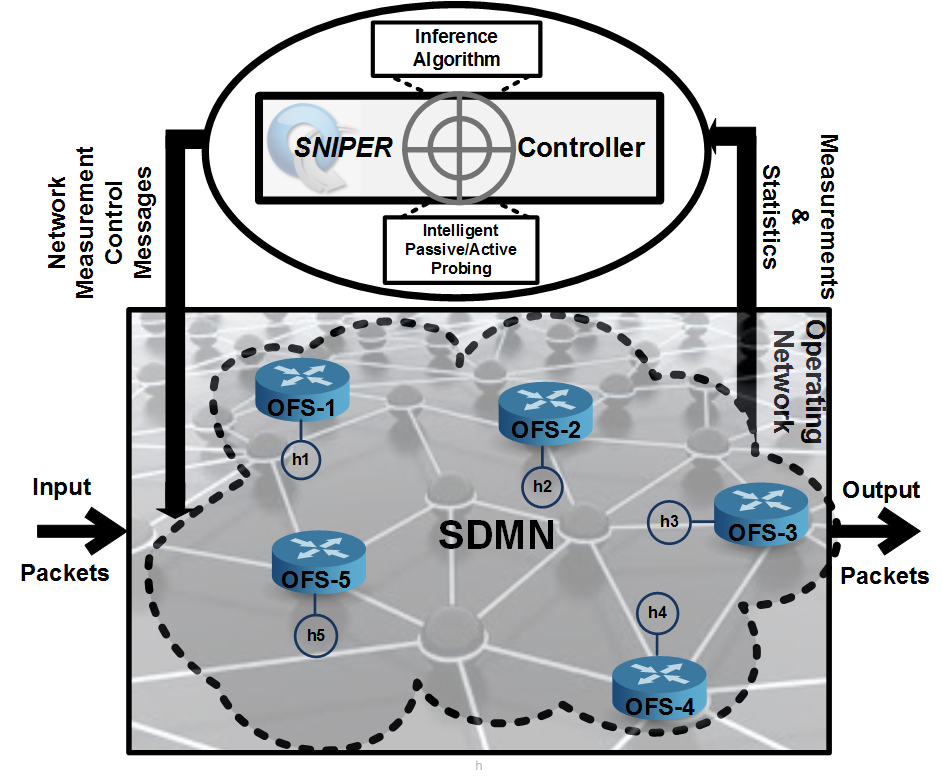
\includegraphics[keepaspectratio, width=0.49\textwidth]{GBDSNIPER_New.png}}
  \end{center}
  \caption{{SNIPER network measurement framework: a general perspective.}}
  \label{fig:GBDSNIPER}
\end{figure}
\begin{figure}[t]
  \begin{center}
    {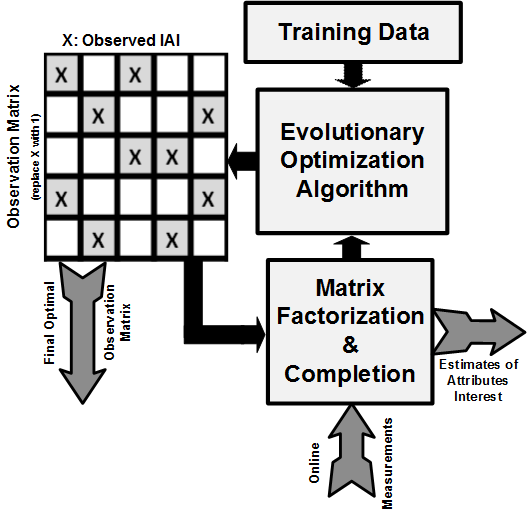
\includegraphics[keepaspectratio, width=0.35\textwidth]{EVSmpMC.png}} \\  % png
  \end{center}
  \caption{{Evolutionary optimal network probing process.}}
  \label{fig:EVSmpMC}
\end{figure}

% For passive measurement (e.g. per-flow size) the flow-tables of the SDMN is adaptively reconfigured. However, for active measurements (e.g. per-flow delay/loss) an appropriate path is first determined and flow-tables of the SDMN is adaptively reconfigured; then, probing packets are injected and routed, and required IAI are measured.
%The SNIPER controller can both preconfigure or adaptively reconfigure the flow-tables of the OFSs in SDMN. For passive per-flow size measurement, the flow-tables of the SDMN are configured and per-flow counter statistics are measured to form the matrix of per-flow sizes. In this case, ONMC messages (here, defined as passive probes) reconfigure the OFSs of the SDMN by installing different rules in flow tables and defining the required actions on the incoming packets of the operating network. 

The SNIPER controller can both pre-program or adaptively reprogram the
flow-tables of the OFSs in SDMN. For passive per-flow size
measurement, NMC messages (defined as passive probes, here)
reconfigure the OFSs of the SDMN by installing required OpenFlow rules
with appropriate forwarding actions in the flow tables for the
incoming packets. The controller also requests and collects per-flow
counter statistics to measure and reconstruct the matrix of per-flow
sizes. On the other hand, for active network performance measurements
(e.g. per-flow delay/loss/throughput), appropriate paths are first
determined (for all required entries of the matrix of IAI). Then, NMC
messages are used to actively probe the operating network by: 1)
adaptively configuring the flow-tables of the SDMN and their
forwarding actions for probing packets sent by a set of hosts; 2)
interacting with the injected probing packets into the network at the
origin of the paths, and 3) collecting required measurements at
destinations. Accordingly, the SNIPER can compute the required IAI and
obtain information of active flows and monitor the end-to-end network
performance measurements. These measurements are transmitted to the
SNIPER controller where matrix completion techniques are used as the
main NI algorithm to estimate all unknown IAI. In SNIPER, since MC
techniques only need partial measurements, not only the communication
overhead between switches and controller is low but also the amount of
network resources used for passive per-flow size measurements
(i.e. TCAM entries) and for active per-flow performance measurements
(mainly required probing bandwidth) are low.

%The measurements are transmitted to the SNIPER controller where matrix completion techniques are used as the main NI algorithm to estimate all unknown IAI. The SNIPER controller can both preconfigure the switches with forwarding rules as well as it can reactively respond to requests from switches, which are sent when a packet matches none of the existing rules enters the network. Besides managing the forwarding plane, the SNIPER controller is also capable of requesting per-flow counter statistics and injecting packets into the network. Accordingly, the SNIPER architecture can obtain information of running flows and regularly injects packets into the network to monitor end-to-end network performance measurements \cite{IF14iSTAMP:2014}\cite{Adrichen:2014}. In this framework, the communication overhead between switches and controller is low, since MC techniques only needs partial measurements. 
% In fact, under the very hard constraints of measurement resources in network monitoring applications, this framework acts as a SNIPER which precisely captures/targets the ONPs. Accordingly, the IAI can be computed because communication networks share a variety of resources of the communication infrastructure (at different layers), and accordingly, there are spatial-temporal correlations/structures \cite{Roughan:2012}\cite{YLiao:2011}\cite{Gursun:2011} that can be used by the NI algorithm to improve the estimation accuracy in inferring IAI.

The feasibility of such Software-Defined Measurement (SDM) frameworks
have been independently investigated in \cite{IF14iSTAMP:2014} and
\cite{Adrichen:2014} where the capability of OpenFlow switches can be
effectively utilized to measure and infer the IAI of the operating
network. Likewise, the SNIPER controller is capable of providing: 1)
per-flow sizes \cite{IF14iSTAMP:2014} by installing the flow ID
prefixes in the flow tables and poll the statistics; 2) per-flow
throughput \cite{Adrichen:2014} by determining specific path for each
flow and query switches to retrieve per-flow statistics where each
query determines the amount of bytes sent and the duration of each
flow; 3) per-flow packet loss \cite{Adrichen:2014} by polling flow
statistics from the first and last switch of each path and subtracting
the increase of the source switch packet counter with the increase of
the packet counter of the destination switch, and 4) per-flow delay
\cite{Adrichen:2014} by assigning a specific path to each flow and
regularly injecting packets into the first switch and having the last
switch send them back to the controller where the difference between
the packet's departure and arrival times are computed by subtracting
the estimated latency from the switch-to-controller delays. This paper
focuses on studying the performance of the SNIPER framework using two
main applications: per-flow size and delay estimations.
% For the details of the implementation please refer to \cite{IF14iSTAMP:2014} and \cite{Adrichen:2014}.
% In this paper, the performance of the SNIPER framework is mainly examined in two main applications including per-flow size and delay estimations using both synthetic and real network measurement traces from different network topologies. In addition, a prototype of SNIPER is implemented in the Mininet to demonstrate its implementation's feasibility and effectiveness.

\subsection{SNIPER: Problem Statement}   \label{subsec:ProbState}
The operating network is modeled as a connected undirected graph $G(V,E)$ where $|V|=N$, and $|E|=m$. Accordingly, there are $m$ links, and $n=N(N-1)$ paths and flows in the network, assuming that there exists an unique path between any pair of nodes in the network. As mentioned in the introduction, we model the NI problem as a Matrix Completion (MC) problem where the goal is to complete the matrix of attributes of interest ($X$) from the direct measurement of a sub-set of its entries assuming that $X$ is a low-rank matrix which contains redundancies and thus not all of its entries are needed to represent it. Here, $X$ is a matrix of size $n \times \mathcal{T}$ ($\mathcal{T}<n$) with rank $r << \mathcal{T}$ where $K$ entries of $X$ is directly measured. 
% The quantity $K$ is defined as $K=s.(n.\mathcal{T})$ where $s$ is the sampling ratio and $0 \leq s \leq 1$.
% In many network monitoring applications, the most important Internal Attributes of Interests (IAI) or performance metrics are flow size, flow throughput, packet loss and delay. Under hard resource constraints of network measurement resources (such as limited processing power and storage capacity, limited number of TCAM entries or limited bandwidth available in active loss/delay measurements) a Network Inference (NI) problem is defined as the process of estimating the IAIs based on a limited set of end-to-end or per-IAI's measurements.
% from just $O(n^{b} r log(n))$ \emph{randomly} observed entries, where $b$ is only slightly larger than 1. 

The theory of matrix completion \cite{Candes:2009} shows that under some suitable conditions, with high probability, $X$ can be exactly recovered from a set of sufficient \emph{randomly} observed entries. In practice, $X$ is often full rank but
with a rank $r$ dominant component, that is, $X$ has only $r$ significant singular values $\sigma_{1}$,..., $\sigma_{r}$ (where $\sigma_{1} \leq ... \leq \sigma_{r}$) and the others are negligible. In such cases, by minimizing the rank, a matrix of rank $r$ (denoted by $\hat{X}$) can still be found that approximates $X$ with high accuracy \cite{YLiao:2011}\cite{Candes:2009}\cite{Keshavan:2009}. Since direct minimization of the rank of a matrix is difficult, MC problems is often formulated as a convex optimization problem Eq.(\ref{MCFormu1}) where $\Omega$ is the set of observed (i.e. directly measured) entries, $P_{\Omega}$ is a sampling function that preserves entries of $X$ in $\Omega$ (i.e. $[P_{\Omega}(X)]_{ij}=x_{ij}$) and turns the others into zero, and $L(X,\hat{X}):=\sum_{i,j=1}^{n} (x_{ij}-\hat{x}_{ij})^{2}$. Corresponding to the sampling function $P_{\Omega}$, a Binary Observation Matrix $S_{\Omega}$ is also defined where $[S_{\Omega}(X)]_{ij}=1$. Accordingly, the MC searches for a low-rank matrix $\hat{X}$ that approximates $X$ with sufficient accuracy at the observed entries in $\Omega$. The unobserved or missing entries in $X$ (indicated by $\bar{\Omega}$ as the complement of $\Omega$) are predicted by the corresponding entries in $\hat{X}$. The MC problem can also be reformulated as a matrix factorization problem in Eq.(\ref{MCFormu2}) where $\hat{X}$ (with $rank(\hat{X}) \leq r$) is factorized as $\hat{X}=U_{n \times r}V_{r \times n}^{T}$ and $\lambda$ is the regularization coefficient that controls the extent of regularization. Here, the Frobenius norm of a matrix $Z$ is defined as $\left\|Z\right\|_{F}^{2}=\sum_{i,j=1}^{n} \left|z_{ij}\right|^{2}$. 

%Different methods can be used to solve optimization problem Eq.(\ref{MCFormu2}).
%The optimization problem Eq.(\ref{MCFormu2}) can be solved using different methods. 
\begin{equation}\label{MCFormu1}
%\small{
\begin{aligned}
\text{minimize} & \hspace{0.25cm} Trace \left( \hat{X} \right) = \sum_{i=1}^{n} \sigma_{i} \\
\text{s.t.} &  \hspace{0.25cm}  L\left(P_{\Omega}(X),P_{\Omega}(\hat{X})\right) \leq \delta
\end{aligned}
%}
\end{equation}

\begin{equation}\label{MCFormu2}
%\small{
\begin{aligned}
\underset{U,V}{\text{minimize}} & \hspace{0.25cm} L\left(P_{\Omega}(X),P_{\Omega}(\hat{X})\right) + \lambda ( \left\|U\right\|_{F}^{2} + \left\|V\right\|_{F}^{2} ) 
\end{aligned}
%}
\end{equation}

The optimization problem Eq.(\ref{MCFormu2}) can be solved using different methods. In this paper, we adopt two different methods from recently proposed MC procedures used in network monitoring applications to solve Eq.(\ref{MCFormu2}) and compute $U$ and $V$ matrices where $\hat{X}=UV^{T}$. The first one is the Sparsity Regularized Singular Value Decomposition (SRSVD) method \cite{Roughan:2012} that uses an alternating least squares procedure to solve Eq.(\ref{MCFormu2}). The second one is the Decentralized Matrix Factorization algorithm \cite{YLiao:2011},denoted by DMFSGD, that uses the Stochastic Gradient Descent (SGD) technique to solve Eq.(\ref{MCFormu2}). Both methods rely on the fact that the matrices of IAI in network monitoring applications contain temporal and/or spatial redundancies that can be used to estimate non-observed or missed entries.

Under hard resource constraints, it is crucial to design OOM, which leads to the best achievable estimation accuracy using matrix completion techniques. To show the importance of such a design, consider a 3$\times$3 matrix $X$ consisting of three spatial-independent processes in each row where $x_{1}(t)=\frac{1}{2}(x_{1}(t-1)+x_{1}(t+1))$, $x_{2}(t)=2x_{2}(t-1)+3$ and $x_{3}(t)=\frac{1}{2} x_{3}(t+1)-10$. Using the temporal structure in these processes, an OOM can be designed as $\Omega_{Opt}=[1, 0, 1; 1, 0, 0; 0, 0, 1]$ where there is at least one 1 in each row. Note that such an OOM can not guaranteed to be obtained using a random sampling strategy.

To maximize the performance of MC algorithms with minimum number of required measurements, such the process of designing the OOM must directly target the ultimate estimation accuracy in the network monitoring applications as defined in Eq.(\ref{NormMetrics}). However, it is extremely complicated, if it is not impossible, to formulate the MC process and target the ultimate performance criterion using a closed-form and well-defined mathematical optimization problem as a function of the observation matrix. In addition, since the observation matrix in our case is a binary matrix, it is computationally expensive and intractable to use integer optimization techniques in such a design process for large-scale networks. Therefore, in this paper, to cope with the inherent complexity of the process of designing large-scale optimal observation matrices, we apply well known evolutionary optimization algorithms that are suitable for optimization problems similar to ours.

%To maximize the performance of NI algorithms with minimum number of required measurements, such a design process must directly target the ultimate estimation accuracy in the network monitoring application. However, it is extremely complicated and computationally complex, if it is not impossible or intractable, to formulate the ultimate performance criteria using a closed-form and well-defined mathematical objective function and solve the problem using regular integer optimization techniques. Therefore, in this paper, to cope with the inherent complexity of the process of designing large-scale optimal observation matrices, we use the well known evolutionary optimization algorithms that are suitable for the optimization problems where the main objective function is a procedure or an algorithm.
%\subsection{Evolutionary-Optimal Observation Matrix Design}
%Evolutionary algorithms are the sub-category of heuristic optimization methods \cite{Talib:2009} for solving NP-hard optimization problems where the main objective function may not be formulated as a well-defined mathematical function. As Figure \ref{fig:} \cite{Kachitvichyanuku:2012} shows, evolutionary algorithms consists of three main processes. The first process is the initialization process where the initial population of individuals is randomly generated according to some solution representation. Each individual represents a solution, directly or indirectly. If an indirect representation is used, each individual must be decoded into a solution. In the second process, each solution in the population is then evaluated for a fintness value. The fitness values can be used to calculate the average population for the purpose of selection. The third process is the generation of a new population by perturbation of solutions in the existing population. The algorithm is run until one or more of the stopping criteria are met. In this paper we use two EAs namely as Genetic Algorithm (GA) and Particle Swarm Optimization (PSO) which have been applied to many optimization and machine learning problems \cite{Talib:2009}\cite{Kachitvichyanuku:2012}.
%
%The main idea of GA is to mimic the natural selection mechanism and the survival of the fittest. In GA, the solutions are represented as chromosomes. The chromosomes are evaluated for fitness values and they are ranked from the best to the worst based on fitness value. The process to produce new solutions in GA is accomplished through three genetic operators as selection, crossover, and mutation. First, the better chromosomes are selected as parents to generate new offspring (new chromosomes). To simulate the survivor of the fittest, the chromosomes with better fitness are selected with higher probabilities. Once the parent chromosomes are selected, the crossover operator combines the chromosomes of the parents to produce new offspring (perturbation of old solutions). To avoid stagnation in the process of evolution, the mutation operator is performed on the chromosomes to increase the diversity of the population. To successfully apply the GA the solution representation (i.e. chromosome model) must be designed carefully. Also, the parent selection process, and the probability of crossover and mutation are important parameters that must be precisely chosen \cite{Kachitvichyanuku:2012}.
%
%In PSO, a solution is represented as a particle, and the population of solutions is called a swarm of particles. The first process in PSO is the initialization process whereby the initial swarm of particles is generated. Each particle is initialized with a random position and velocity. Each particle is then evaluated for fitness value. Each time a fitness value is calculated, it is compared against the previous best fitness value of the particle and the previous best fitness value of the whole swarm, and, accordingly, the personal best and global best positions are updated, appropriately. If a stopping criterion is not met, the velocity and position are updated to create a new swarm. The positions and velocities of particles are updated based on the personal best and global best positions, as well as the
%old velocities. It should be noted that PSO algorithm does not require sorting of fitness values of solutions in any process. This might be a significant computational advantage over GA, especially when the population size is large \cite{Kachitvichyanuku:2012} \cite{Eberhart:2001}.
%% The velocity is updated based on three components: the old velocity (inertia or momentum term), experience of an individual particle (cognitive or self learning term), and experience of the whole swarm (group or social learning term). Each term has a weight constant associated with it.
%
%Throughout this paper, the fitness of the solutions in our evolutionary algorithms (chromosome in GA and particle in PSO) are evaluated using the following two metrics, namely, Normalized Mean Absolute Error (NMAE) and Normalized Mean Square Error (NMSE) where $x_{ij}$ denotes the $ij^{th}$ entry of the matrix $X$ (which is known in the learning stage) and $\hat{x}_{ij}$ denotes the $ij^{th}$ entry of the matrix $\hat{X}$ which is output of the MC process. 
%
%\begin{equation} \label{NormMetrics}
%\footnotesize{
%\begin{aligned}
%NMAE = \frac{\sum_{ij \in \bar{\Omega}} \left|x_{ij} - \hat{x}_{ij}\right|}{\sum_{ij \in \bar{\Omega}} \left|x_{ij}\right|} \\
%NMSE = \frac{\sqrt{\sum_{ij \in \bar{\Omega}} \left(x_{ij} - \hat{x}_{ij}\right)^{2} }}{\sqrt{\sum_{ij \in \bar{\Omega}} \left(x_{ij}\right)^{2}}}
%\end{aligned}
%}
%\end{equation}
%
%Here, a solution in the GA is represented as a chromosome which is defined as a binary sampling matrix $C$ with size $n \times \mathcal{T}$ and where $0$ and $1$ respectively represent unobserved and directly measured entries. The number of measurements paths (i.e. samples) for each chromosome is denoted by $K$ (i.e. the number of one's in each chromosome). To successfully apply the MC technique, the sampling matrix $C$ is constrained to have at least one $1$ in each row and column. The GA is started by generating $N_{p}$ chromosomes/solutions in the initialization step. Then, the fitness of each chromosome is evaluated using the cost function Eq.(\ref{NormMetrics}). Accordingly, the best chromosomes, with lowest fitness values, are selected and the crossover operation (as defined in Eq.(\ref{GACrossOver})), with probability $p_{c}$, is applied on each pair of parents to generate new children (offsprings); offsprings form the new chromosomes of the next generation. To increase the diversity of the population, the mutation operation is performed on each child where the mutation operator changes an entry of sampling matrix $C$ from zero-to-one or vice-versa with probability $p_{m}$. The GA process is continued over $N_{i}$ iterations and the best chromosome in each iteration remains unchanged.
%% Among these, the best chromosome remains unchanged; and also, some simple manipulations are applied at each step to keep the number of measurement paths constant for each sampling rate in such a way that chromosomes remain symmetric (if it is required, for example, in the case of delay measurement) with having at least an one in each row/column of $C$ (please refer to \cite{SNIPERTechReport:2014} for further details). The GA process is continued over $N_{i}$ iterations.
%\begin{equation} \label{GACrossOver}
%\footnotesize{
%\begin{aligned}
%\text{OffSpring}_{1} = C_{1}(1:r,:) + C_{2}(r+1:n,:) \\
%\text{OffSpring}_{2} = C_{2}(1:r,:) + C_{1}(r+1:n,:) 
%\end{aligned}
%}
%\end{equation}
%
%Likewise, the PSO is started by generating $N_{p}$ particles where $i^{th}$ particle is identified by its position $P^{k}_{i}$ and velocity $V^{k}_{i}$ at iteration $k$. Here, $P^{k}_{i}$ is an $n \times \mathcal{T}$ binary matrix, representing the measurement matrix, and $V^{k}_{i}$ is also an $n \times \mathcal{T}$ matrix. In the initialization stage all position and velocity matrices are zero matrices. The best position of $i^{th}$ particle obtained until iteration $k$ is denoted by $BP_{i}^{k}$ and the best position among all particles in the swarm until iteration $k$ is called global best position and it is denoted by $GP^{k}$. The best particles here is determined by evaluating the fitness of each particle and choosing the one with the minimum error value (as defined in Eq.(\ref{NormMetrics})) among all iterations (for one particle) or among all particles. 
%
%The velocity $V^{k}_{i}$ is  updated according to Eq.(\ref{PSOPosVlc}) where $c_{1}$ and $c_{2}$ are acceleration constants, which here they setup to $c_{1}=c_{2}=2$, and $\alpha_{1}$ and $\alpha_{2}$ are standard uniform random variables in interval $[0,1]$. The positive inertia weight $\omega$ is computed as  $\omega=\omega_{max}-(\omega_{max}-\omega_{min})\frac{k}{N_{i}}$ where $\omega_{min}$ and $\omega_{max}$ are respectively minimum and maximum inertia weights which, here, we setup to $\omega_{min}=0.3$, $\omega_{max}=0.9$ and $N_{i}=2000$. The particle positions are updated (by re-determining the new measurement paths) using two methods: 1) set the entries $\{p^{k}_{ij}\}_{ij\in I^{V}_{max}}=1$ where $I^{V}_{max}$ indicates the set of $ij^{th}$ entries with highest velocities in the matrix $V^{k}_{i}$ (i.e. $(\sim,I^{V}_{max}=sort(V^{k}_{i}(:))$), and 2) $\{p_{ij}\}$ is set to one with probability $sigmoid(v_{ij})$, where $sigmoid(x):=\frac{1}{1+e^{-x}}$, otherwise it is set to zero. The PSO process is continued over $N_{i}$ iterations.
%
%In both GA and PSO evolutionary algorithms, some simple manipulations are applied at each step to keep the number of measurement paths constant for each sampling rate in such a way that chromosomes/particles remain symmetric (if it is required, for example, in the case of delay measurement) with having at least an one in each row and column of the solution representation (please refer to \cite{SNIPERTechReport:2014} for further details).
%\begin{equation} \label{PSOPosVlc}
%\footnotesize{
%\begin{aligned}
%V_{i}^{k} = \omega V_{i}^{k-1}+c_{1} \alpha_{1} (BP_{i}^{k}-P_{i}^{k-1}) + c_{2} \alpha_{2} (GP^{k}-P_{i}^{k-1}) \\
%\end{aligned}
%}
%\end{equation}














%Now, if 
%
%MC techniques hagofte shavad ba tekieh bar factorization va har do raveshe mghaleha tozih dade shavad.
%
%
%moshkelat inja gofte shavad (ke rabeteii nist beine performance va strcture matrix dar resource constrainted casaes) baad dar section "`EV optimal probing design" jozeyat gofte shavad
%
%
%
% 
%the OFSs  
%
%
%
%
%
%However,
%it is a valid question to ask what the optimal observation
%(i.e. aggregation) matrix is to maximize the performance of
%CS recovery. Such a direct optimization approach for designing
%the optimal observation matrix AOpt
%g , to maximize the
%performance of CS recovery technique, is prohibitive1 due
%to the complexity of the process [24]. Therefore, to simplify
%the process of designing the optimal observation matrix other
%objective functions are considered in the optimization process,
%while accepting the unavoidable sacrifice in performance [24].
%
%
%
%
%
%  
%
%
%
%
% \cite{Candes:2009} shows that under some suitable
%conditions, with high probability, $X$ can be exactly recovered from just $O(n^{b} r log(n))$ randomly
%
%
%
%
%
%
%
%
%
%
%% \subsection{SNIPER: Problem }   \label{subsec:ProbState}
%
%
%
%that leverages the sparse or low-rank nature of real-world traffic matrices and their spatio-temporal properties to interpolate missed traffic entries due to ***
%
%\cite{Roughan:2012}
%
%SPARSITY REGULARIZED MATRIX FACTORIZATION
%
%
%
%
%
%
%
%
%
%To design and evaluate the performance of SNIPER the 
%
%% Since communication networks share a variety of resources of the communication infrastructure (at different layers), then, under the hard constraint of measurement resources, this framework acts as a SNIPER which precisely captures/targets the ONPs. 
%
%% \vspace{10in}
%%
%% to determine the best possible measurements in the next stage. This process evolves over time      
%%
%%and through an adaptive process where the Evolutionary Algorithm (EA) utilizes the statistics/measurements at each stage to determine the best possible measurements in the next stage. This process evolves over time      
%%
%% of i
%%
%%network performance quality.
%%
%%
%%
%%a variety of attributes of interest in the operating network in different time and/or spaces.  
%%
%%
%%
%%
%%
%%including per-flows sizes, link delays, packet losses and link throughputs using both passive and active probing messages. Passive messages consists of required  
%%
%%attribute of interest in SNIPER framework 
%%
%%
%%\begin{equation}\label{ISDNFMOpt2}
%%\small{
%%\begin{aligned}
%%& \hat{X} = \underset{X}{\text{minimize}} \left\|Y^{t}_{S}-HX^{t}_{g}\right\|_{p}^{2} + \lambda \left\|X^{t}_{g}\right\|_{q}\\
%%& \text{s.t.} \hspace{0.25cm} Y^{t}_{g}=A_{g}^{t} X^{t}_{g}, \hspace{0.25cm} X^{t}_{k}=A_{k}^{t} X^{t}_{k}, \hspace{0.25cm} X^{t}_{g} \geq 0\\
%%\end{aligned}
%%}
%%\end{equation}
%%
%%In iSTAMP, the communication overhead between the
%%controller and switch is low because only a few flows are
%%directly measured and other entires are used to aggregate a large
%%number of flows (hence, $T$ instead of $n$ measurement records) which is important under hard resource constraints and in multi-point measurement scenario. iSTAMP is also computationally efficient because it exploits existing low-complexity network inference techniques \cite{YCEldar:2012}.





%
%  that can not be formulated as a well-defined mathematical function.
%
%
%
%
%a closed-form and well-defined mathematical objective function that can be efficiently optimized is extremely complicated and computationally complex.
%
%The direct design of observation matrices for maximizing the performance of NI methods is prohibitive due to the complexity of the process, and therefore, to simplify the process of designing the optimal observation matrix other objective functions are considered in the optimization process, while accepting the unavoidable sacrifice in performance \cite{Elad:2007} \cite{IF14iSTAMP:2014}. The underlying difficulty in this direct optimal observation matrix design is that formulating the network inference process/algorithm into a closed-form and well-defined mathematical objective function that can be efficiently optimized is extremely complicated and computationally complex, if it is not impossible or intractable.
%
%
%
%
%Comparing to random measurement techniques used in the theory of MC, such an optimal design of the observation matrix results in 
%
%
%Under hard resource constraints of network measurement resources, the evolutionary optimization algorithms can be used to directly design the optimal observation or measurement matrix, which leads to the best achievable estimation accuracy via applying matrix completion technique onto the NI problem. Comparing to random measurement techniques used in the theory of MC, such an optimal design of the observation matrix results in 
%
%comapring to random measurement techniques This leads to the fewer or better accuracy
%
%
% how can we optimally measure or sample the entries of the matrix of attributes of interest which leads to the best possible estimation accuracy via using matrix completion techniques?}
%
%
%In the theory of matrix completion, the matrix of the attributes of interest can be completely reconstructed from a sub-set of \emph{randomly} observed entries (i.e. measurements) if the number of observations are \emph{high} enough. Accordingly, in network monitoring applications and by considering the flexibility provided by the SDN, an interesting question that can be asked is: \\
%
%\emph{
%Under hard resource constraints of network measurement resources, how can we optimally measure or sample the entries of the matrix of attributes of interest which leads to the best possible estimation accuracy via using matrix completion techniques?}
% Such an optimal measurement/observation matrix is efficient in the sense that it needs less number of measurements to reach the same estimation accuracy via random measurement scheme, or equivalently, for the same number of measurements the optimal sampling techniques reaches a better perfromance. 
%\vspace{0.15cm}\\
%
%The direct design of observation matrices for maximizing the performance of NI methods is prohibitive due to the complexity of the process, and therefore, to simplify the process of designing the optimal observation matrix other objective functions are considered in the optimization process, while accepting the unavoidable sacrifice in performance \cite{Elad:2007} \cite{IF14iSTAMP:2014}. The underlying difficulty in this direct optimal observation matrix design is that formulating the network inference process/algorithm into a closed-form and well-defined mathematical objective function that can be efficiently optimized is extremely complicated and computationally complex, if it is not impossible or intractable.
%
%Hence, in this paper and to the best of our knowledge for the first time, we change the main approach in designing the optimal observation matrix for network inference problems where we directly target the ultimate estimation accuracy in network monitoring applications in our optimization framework. However, to cope with the inherent complexity of the process of designing large-scale optimal observation matrices, we use the well known evolutionary optimization algorithms that are suitable for the optimization problems where the main objective function is a procedure or an algorithm that can not be formulated as a well-defined mathematical function.
%
% of objective functions that can not be formulated into a closed-form and well-defined mathematical 
% that the objective function can not  
%as the approximate-heuristic optimization method \cite{Talib:2009}. 
%
%\subsection{Evolutionary Algorithms (EA)}

\section{SNIPER: System Description}  \label{sec:SNIPERSysDsc}
In this section we describe various components of our proposed SNIPER framework. Figure \ref{fig:GBDSNIPER} shows the general block diagram
of the SNIPER framework where the controller interacts with Software
Defined Measurement Network (SDMN) using Network
Measurement Controlling (NMC) messages to dynamically program the SDMN
and poll the required measurements and statistics. The SDMN consists
of a set of Probing Agents (PA), for example hosts, which can inject probing packets into the network, and a sub-set of OpenFlow Switches (OFS) in the
operating network. Without loss of generality, we assume that SDMN
guarantees all required IAI are \emph{observable} and
\emph{measurable}. The NMC messages include passive and active network
measurement control messages that indicate which IAI must be
accurately measured at different times and/or locations and setups
appropriate flow-table entries and probe requests in the SDMN,
accordingly. In the SNIPER framework, the network measurement process
is consisted of two stages, namely the learning and measurement
epochs, as it is shown in Figure \ref{fig:EVSmpMC}. In the supervised learning stage the optimal IAI that must be directly measured are precisely computed using an evolutionary optimization algorithm and a training data-set. Then, in the online measurement epoch, the SDN flexibility is used to reconfigure the SDMN and to collect the measurements of corresponding optimal IAI. This framework can also be deployed in
dynamic environments by decreasing its dependency on the initial
training data-set and adaptively updating the optimal observation
matrix.
%This framework can also be equipped with online EOAs where measurement and learning are concurrently performed without using the training data.
% \footnote{For optimal network monitor placement problem, please refer to \cite{LMa1:2014}, \cite{LMa2:2014} and \cite{XWang:2014}.}
%The SNIPER framework provides the ability of measuring a sub-set of the precisely chosen attributes of interest (called Optimal Network Probes (ONP)) of the operating network at different times and/or spaces which resulted in the best possible accuracy in estimating the set of all unknown attributes of interests.
\begin{figure}[t]
  \begin{center}
    {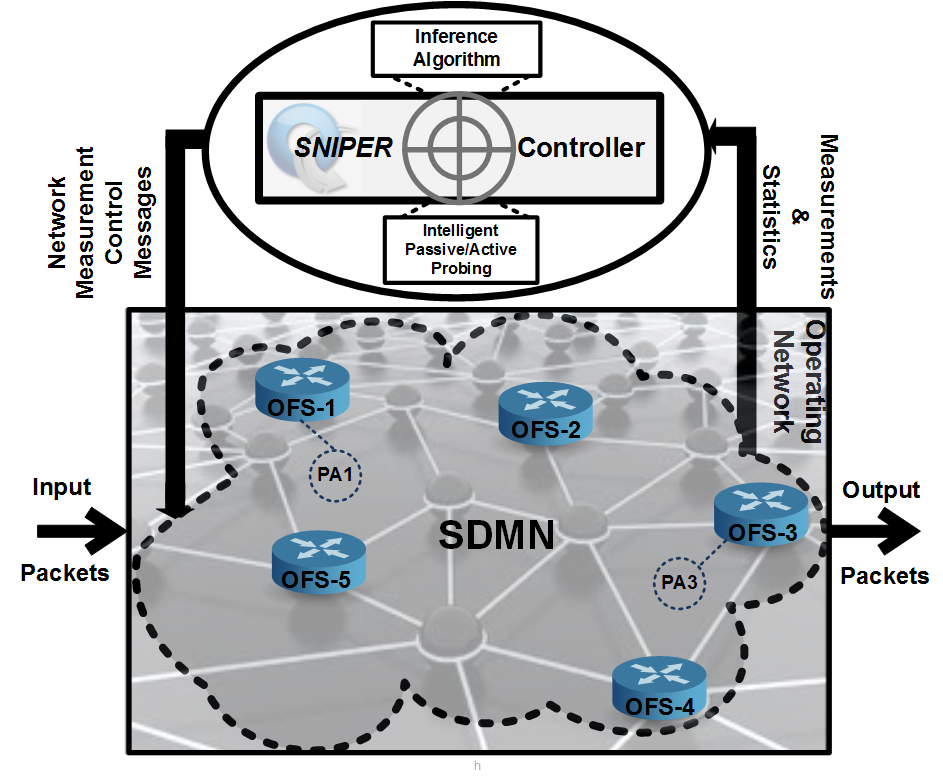
\includegraphics[keepaspectratio, width=0.42\textwidth]{GBDSNIPER_New2.png}}
  \end{center}
  \caption{{SNIPER network measurement framework: a general perspective.}}
  \label{fig:GBDSNIPER}
\end{figure}
\begin{figure}[t]
  \begin{center}
    {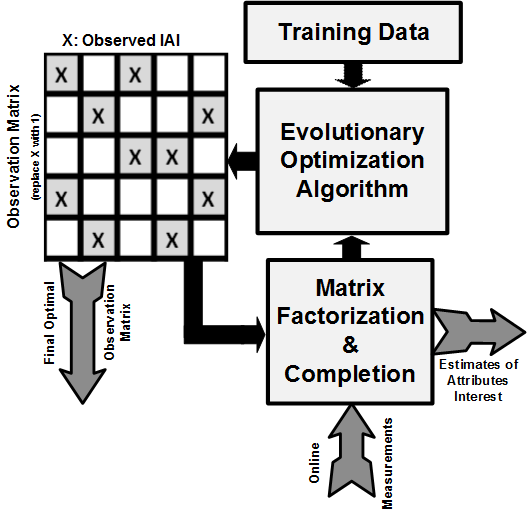
\includegraphics[keepaspectratio, width=0.28\textwidth]{EVSmpMC.png}} \\  % png
  \end{center}
  \caption{{Evolutionary optimal network measurement and inference process.}}
  \label{fig:EVSmpMC}
\end{figure}

% For passive measurement (e.g. per-flow size) the flow-tables of the SDMN is adaptively reconfigured. However, for active measurements (e.g. per-flow delay/loss) an appropriate path is first determined and flow-tables of the SDMN is adaptively reconfigured; then, probing packets are injected and routed, and required IAI are measured.
%The SNIPER controller can both preconfigure or adaptively reconfigure the flow-tables of the OFSs in SDMN. For passive per-flow size measurement, the flow-tables of the SDMN are configured and per-flow counter statistics are measured to form the matrix of per-flow sizes. In this case, ONMC messages (here, defined as passive probes) reconfigure the OFSs of the SDMN by installing different rules in flow tables and defining the required actions on the incoming packets of the operating network. 
The SNIPER controller can both pre-configure or adaptively reconfigure the
flow-tables of the OFSs in SDMN. For passive per-flow size
measurement, NMC messages (defined as passive probes, here)
reconfigure the OFSs of the SDMN by installing required OpenFlow rules
with appropriate forwarding actions in the flow tables for the
incoming packets. The controller also requests and collects per-flow
counter statistics to measure and reconstruct the matrix of per-flow
sizes. On the other hand, for active network performance measurements
(e.g. per-flow delay/loss/throughput), appropriate paths are first
determined (for all required entries of the matrix of IAI). Then, NMC
messages are used to actively probe the operating network by: 1)
adaptively configuring the flow-tables of the SDMN and their
forwarding actions for probing packets sent by a set of probing agents; 2)
interacting with the injected probing packets into the network at the
origin of the paths, and 3) collecting required measurements at
destinations. Accordingly, the SNIPER can compute the required IAI and
obtain information of active flows and monitor the end-to-end network
performance measurements. These measurements are transmitted to the
SNIPER controller where matrix completion techniques are used as the
main NI algorithm to estimate all unknown IAI. In SNIPER, since MC
techniques only need partial measurements, not only the communication
overhead between switches and controller is low but also the amount of
network resources used for passive per-flow size measurements
(i.e. TCAM entries) and for active per-flow performance measurements
(mainly required probing bandwidth) are low. In addition, the computational overhead of the SNIPER is low as efficient algorithms are used for implementing MC and EOAs \cite{Roughan:2012}\cite{YLiao:2011}\cite{Kachitvichyanuku:2012}. 

%The measurements are transmitted to the SNIPER controller where matrix completion techniques are used as the main NI algorithm to estimate all unknown IAI. The SNIPER controller can both preconfigure the switches with forwarding rules as well as it can reactively respond to requests from switches, which are sent when a packet matches none of the existing rules enters the network. Besides managing the forwarding plane, the SNIPER controller is also capable of requesting per-flow counter statistics and injecting packets into the network. Accordingly, the SNIPER architecture can obtain information of running flows and regularly injects packets into the network to monitor end-to-end network performance measurements \cite{IF14iSTAMP:2014}\cite{Adrichen:2014}. In this framework, the communication overhead between switches and controller is low, since MC techniques only needs partial measurements. 
% In fact, under the very hard constraints of measurement resources in network monitoring applications, this framework acts as a SNIPER which precisely captures/targets the ONPs. Accordingly, the IAI can be computed because communication networks share a variety of resources of the communication infrastructure (at different layers), and accordingly, there are spatial-temporal correlations/structures \cite{Roughan:2012}\cite{YLiao:2011}\cite{Gursun:2011} that can be used by the NI algorithm to improve the estimation accuracy in inferring IAI.

The feasibility of such Software-Defined Measurement (SDM) frameworks
have been independently investigated in \cite{IF14iSTAMP:2014} and
\cite{Adrichen:2014} where the capability of OpenFlow switches can be
effectively utilized to measure and infer the IAI of the operating
network. Likewise, the SNIPER controller is capable of providing: 1)
per-flow sizes \cite{IF14iSTAMP:2014} by installing the flow ID
prefixes in the flow tables and poll the statistics; 2) per-flow
throughput \cite{Adrichen:2014} by determining specific path for each
flow and query switches to retrieve per-flow statistics where each
query determines the amount of bytes sent and the duration of each
flow; 3) per-flow packet loss \cite{Adrichen:2014} by polling flow
statistics from the first and last switch of each path and subtracting
the increase of the source switch packet counter with the increase of
the packet counter of the destination switch, and 4) per-flow delay
\cite{Adrichen:2014} by assigning a specific path to each flow and
regularly injecting packets into the first switch and having the last
switch send them back to the controller where the difference between
the packet's departure and arrival times are computed by subtracting
the estimated latency from the switch-to-controller delays. 

This paper focuses on studying the performance of the SNIPER framework in two
main applications: per-flow size and delay estimations.
% For the details of the implementation please refer to \cite{IF14iSTAMP:2014} and \cite{Adrichen:2014}.
% In this paper, the performance of the SNIPER framework is mainly examined in two main applications including per-flow size and delay estimations using both synthetic and real network measurement traces from different network topologies. In addition, a prototype of SNIPER is implemented in the Mininet to demonstrate its implementation's feasibility and effectiveness.

\subsection{SNIPER: Problem Statement}   \label{subsec:ProbState}
The operating network is modeled as a connected undirected graph $G(V,E)$ where $|V|=N$, and $|E|=m$. Accordingly, there are $m$ links, and $n=N(N-1)$ paths and flows in the network, assuming that there exists an unique path between any pair of nodes in the network. As mentioned in the introduction, we model the NI problem as a Matrix Completion (MC) problem where the goal is to complete the matrix of IAI ($X$) from the direct measurement of a sub-set of its entries assuming that $X$ is a low-rank matrix which contains redundancies and thus not all of its entries are needed to represent it. Here, $X$ is an $n \times T_{0}$ matrix with rank $r << T_{0}$ and $T_{0}<n$ where $K$ entries of $X$ is directly measured. 
% The quantity $K$ is defined as $K=s.(n.\mathcal{T})$ where $s$ is the sampling ratio and $0 \leq s \leq 1$.
% In many network monitoring applications, the most important Internal Attributes of Interests (IAI) or performance metrics are flow size, flow throughput, packet loss and delay. Under hard resource constraints of network measurement resources (such as limited processing power and storage capacity, limited number of TCAM entries or limited bandwidth available in active loss/delay measurements) a Network Inference (NI) problem is defined as the process of estimating the IAIs based on a limited set of end-to-end or per-IAI's measurements.
% from just $O(n^{b} r log(n))$ \emph{randomly} observed entries, where $b$ is only slightly larger than 1. 

The theory of matrix completion \cite{Candes:2009} shows that under some suitable conditions, with high probability, $X$ can be exactly recovered from a set of sufficient \emph{randomly} observed entries. In practice, $X$ is often full rank but
with a rank $r$ dominant component, that is, $X$ has only $r$ significant singular values $\sigma_{1}$,..., $\sigma_{r}$ (where $\sigma_{1} \leq ... \leq \sigma_{r}$) and the others are negligible. In such cases, by minimizing the rank, a matrix of rank $r$ (denoted by $\hat{X}$) can still be found that approximates $X$ with high accuracy \cite{YLiao:2011}\cite{Candes:2009}\cite{Keshavan:2009}. Since direct minimization of the rank of a matrix is difficult, MC problems is often formulated as a convex optimization problem Eq.(\ref{MCFormu1}) where $\Omega$ is the set of observed (i.e. directly measured) entries, $P_{\Omega}$ is a sampling function that preserves entries of $X$ in $\Omega$ (i.e. $[P_{\Omega}(X)]_{ij}=x_{ij}$) and turns the others into zero, and $L(X,\hat{X}):=\sum_{i,j=1}^{n} (x_{ij}-\hat{x}_{ij})^{2}$. Corresponding to the sampling function $P_{\Omega}$, a Binary Observation Matrix $S_{\Omega}$ is also defined where $[S_{\Omega}(X)]_{ij}=1$. Accordingly, the MC searches for a low-rank matrix $\hat{X}$ that approximates $X$ with sufficient accuracy at the observed entries in $\Omega$. The unobserved or missing entries in $X$ (indicated by $\bar{\Omega}$ as the complement of $\Omega$) are predicted by the corresponding entries in $\hat{X}$. The MC problem can also be reformulated as a matrix factorization problem in Eq.(\ref{MCFormu2}) where $\hat{X}$ (with $rank(\hat{X}) \leq r$) is factorized as $\hat{X}=U_{n \times r}V_{r \times n}^{T}$ and $\lambda$ is the regularization coefficient that controls the extent of regularization. Here, the Frobenius norm of a matrix $Z$ is defined as $\left\|Z\right\|_{F}^{2}=\sum_{i,j=1}^{n} \left|z_{ij}\right|^{2}$. 
%Different methods can be used to solve optimization problem Eq.(\ref{MCFormu2}).
%The optimization problem Eq.(\ref{MCFormu2}) can be solved using different methods. 
\begin{equation}\label{MCFormu1}
%\small{
\begin{aligned}
\text{minimize} & \hspace{0.25cm} Trace \left( \hat{X} \right) = \sum_{i=1}^{n} \sigma_{i} \\
\text{s.t.} &  \hspace{0.25cm}  L\left(P_{\Omega}(X),P_{\Omega}(\hat{X})\right) \leq \delta
\end{aligned}
%}
\end{equation}
\begin{equation}\label{MCFormu2}
%\small{
\begin{aligned}
\underset{U,V}{\text{minimize}} & \hspace{0.25cm} L\left(P_{\Omega}(X),P_{\Omega}(\hat{X})\right) + \lambda ( \left\|U\right\|_{F}^{2} + \left\|V\right\|_{F}^{2} ) 
\end{aligned}
%}
\end{equation}

The optimization problem Eq.(\ref{MCFormu2}) can be solved using different methods. In this paper, we adopt two different methods from recently proposed MC procedures used in network monitoring applications to solve Eq.(\ref{MCFormu2}) and compute $U$ and $V$ matrices where $\hat{X}=UV^{T}$. The first one is the Sparsity Regularized Singular Value Decomposition (SRSVD) method \cite{Roughan:2012} that uses an alternating least squares procedure to solve Eq.(\ref{MCFormu2}). The second one is the Decentralized Matrix Factorization algorithm \cite{YLiao:2011},denoted by DMFSGD, that uses the Stochastic Gradient Descent (SGD) technique to solve Eq.(\ref{MCFormu2}). Both methods rely on the fact that the matrices of IAI in network monitoring applications contain temporal and/or spatial redundancies that can be used to estimate non-observed or missed entries. Note that, SNIPER is a flexible framework that can be equipped with more advanced MC algorithms with better performance.  

Under hard resource constraints, it is crucial to design OOM, which leads to the best achievable estimation accuracy using matrix completion techniques. To show the importance of such a design, consider a 3$\times$3 matrix $X$ consisting of three spatial-independent processes in each row where $x_{1}(t)=\frac{1}{2}(x_{1}(t-1)+x_{1}(t+1))$, $x_{2}(t)=2x_{2}(t-1)+3$ and $x_{3}(t)=\frac{1}{2} x_{3}(t+1)-10$. Using the temporal structure in these processes, an OOM can be designed as $\Omega_{Opt}=[1, 0, 1; 1, 0, 0; 0, 0, 1]$ where there is at least one 1 in each row. Note that such an OOM can not guaranteed to be obtained using a random sampling strategy.

To maximize the performance of MC algorithms with minimum number of required measurements, such the process of designing the OOM must directly target the ultimate estimation accuracy in the network monitoring applications as defined in Eq.(\ref{NormMetrics}). However, it is extremely complicated, if it is not impossible, to formulate the MC process and target the ultimate performance criterion using a closed-form and well-defined mathematical optimization problem as a function of the observation matrix. In addition, since the observation matrix in our case is a binary matrix, it is computationally expensive and intractable to use integer optimization techniques in such a design process for large-scale networks. Therefore, in this paper, to cope with the inherent complexity of the process of designing large-scale optimal observation matrices, we apply well known evolutionary optimization algorithms that are suitable for optimization problems similar to ours.

%To maximize the performance of NI algorithms with minimum number of required measurements, such a design process must directly target the ultimate estimation accuracy in the network monitoring application. However, it is extremely complicated and computationally complex, if it is not impossible or intractable, to formulate the ultimate performance criteria using a closed-form and well-defined mathematical objective function and solve the problem using regular integer optimization techniques. Therefore, in this paper, to cope with the inherent complexity of the process of designing large-scale optimal observation matrices, we use the well known evolutionary optimization algorithms that are suitable for the optimization problems where the main objective function is a procedure or an algorithm.
%\subsection{Evolutionary-Optimal Observation Matrix Design}
%Evolutionary algorithms are the sub-category of heuristic optimization methods \cite{Talib:2009} for solving NP-hard optimization problems where the main objective function may not be formulated as a well-defined mathematical function. As Figure \ref{fig:} \cite{Kachitvichyanuku:2012} shows, evolutionary algorithms consists of three main processes. The first process is the initialization process where the initial population of individuals is randomly generated according to some solution representation. Each individual represents a solution, directly or indirectly. If an indirect representation is used, each individual must be decoded into a solution. In the second process, each solution in the population is then evaluated for a fintness value. The fitness values can be used to calculate the average population for the purpose of selection. The third process is the generation of a new population by perturbation of solutions in the existing population. The algorithm is run until one or more of the stopping criteria are met. In this paper we use two EAs namely as Genetic Algorithm (GA) and Particle Swarm Optimization (PSO) which have been applied to many optimization and machine learning problems \cite{Talib:2009}\cite{Kachitvichyanuku:2012}.
%
%The main idea of GA is to mimic the natural selection mechanism and the survival of the fittest. In GA, the solutions are represented as chromosomes. The chromosomes are evaluated for fitness values and they are ranked from the best to the worst based on fitness value. The process to produce new solutions in GA is accomplished through three genetic operators as selection, crossover, and mutation. First, the better chromosomes are selected as parents to generate new offspring (new chromosomes). To simulate the survivor of the fittest, the chromosomes with better fitness are selected with higher probabilities. Once the parent chromosomes are selected, the crossover operator combines the chromosomes of the parents to produce new offspring (perturbation of old solutions). To avoid stagnation in the process of evolution, the mutation operator is performed on the chromosomes to increase the diversity of the population. To successfully apply the GA the solution representation (i.e. chromosome model) must be designed carefully. Also, the parent selection process, and the probability of crossover and mutation are important parameters that must be precisely chosen \cite{Kachitvichyanuku:2012}.
%
%In PSO, a solution is represented as a particle, and the population of solutions is called a swarm of particles. The first process in PSO is the initialization process whereby the initial swarm of particles is generated. Each particle is initialized with a random position and velocity. Each particle is then evaluated for fitness value. Each time a fitness value is calculated, it is compared against the previous best fitness value of the particle and the previous best fitness value of the whole swarm, and, accordingly, the personal best and global best positions are updated, appropriately. If a stopping criterion is not met, the velocity and position are updated to create a new swarm. The positions and velocities of particles are updated based on the personal best and global best positions, as well as the
%old velocities. It should be noted that PSO algorithm does not require sorting of fitness values of solutions in any process. This might be a significant computational advantage over GA, especially when the population size is large \cite{Kachitvichyanuku:2012} \cite{Eberhart:2001}.
%% The velocity is updated based on three components: the old velocity (inertia or momentum term), experience of an individual particle (cognitive or self learning term), and experience of the whole swarm (group or social learning term). Each term has a weight constant associated with it.
%
%Throughout this paper, the fitness of the solutions in our evolutionary algorithms (chromosome in GA and particle in PSO) are evaluated using the following two metrics, namely, Normalized Mean Absolute Error (NMAE) and Normalized Mean Square Error (NMSE) where $x_{ij}$ denotes the $ij^{th}$ entry of the matrix $X$ (which is known in the learning stage) and $\hat{x}_{ij}$ denotes the $ij^{th}$ entry of the matrix $\hat{X}$ which is output of the MC process. 
%
%\begin{equation} \label{NormMetrics}
%\footnotesize{
%\begin{aligned}
%NMAE = \frac{\sum_{ij \in \bar{\Omega}} \left|x_{ij} - \hat{x}_{ij}\right|}{\sum_{ij \in \bar{\Omega}} \left|x_{ij}\right|} \\
%NMSE = \frac{\sqrt{\sum_{ij \in \bar{\Omega}} \left(x_{ij} - \hat{x}_{ij}\right)^{2} }}{\sqrt{\sum_{ij \in \bar{\Omega}} \left(x_{ij}\right)^{2}}}
%\end{aligned}
%}
%\end{equation}
%
%Here, a solution in the GA is represented as a chromosome which is defined as a binary sampling matrix $C$ with size $n \times \mathcal{T}$ and where $0$ and $1$ respectively represent unobserved and directly measured entries. The number of measurements paths (i.e. samples) for each chromosome is denoted by $K$ (i.e. the number of one's in each chromosome). To successfully apply the MC technique, the sampling matrix $C$ is constrained to have at least one $1$ in each row and column. The GA is started by generating $N_{p}$ chromosomes/solutions in the initialization step. Then, the fitness of each chromosome is evaluated using the cost function Eq.(\ref{NormMetrics}). Accordingly, the best chromosomes, with lowest fitness values, are selected and the crossover operation (as defined in Eq.(\ref{GACrossOver})), with probability $p_{c}$, is applied on each pair of parents to generate new children (offsprings); offsprings form the new chromosomes of the next generation. To increase the diversity of the population, the mutation operation is performed on each child where the mutation operator changes an entry of sampling matrix $C$ from zero-to-one or vice-versa with probability $p_{m}$. The GA process is continued over $N_{i}$ iterations and the best chromosome in each iteration remains unchanged.
%% Among these, the best chromosome remains unchanged; and also, some simple manipulations are applied at each step to keep the number of measurement paths constant for each sampling rate in such a way that chromosomes remain symmetric (if it is required, for example, in the case of delay measurement) with having at least an one in each row/column of $C$ (please refer to \cite{SNIPERTechReport:2014} for further details). The GA process is continued over $N_{i}$ iterations.
%\begin{equation} \label{GACrossOver}
%\footnotesize{
%\begin{aligned}
%\text{OffSpring}_{1} = C_{1}(1:r,:) + C_{2}(r+1:n,:) \\
%\text{OffSpring}_{2} = C_{2}(1:r,:) + C_{1}(r+1:n,:) 
%\end{aligned}
%}
%\end{equation}
%
%Likewise, the PSO is started by generating $N_{p}$ particles where $i^{th}$ particle is identified by its position $P^{k}_{i}$ and velocity $V^{k}_{i}$ at iteration $k$. Here, $P^{k}_{i}$ is an $n \times \mathcal{T}$ binary matrix, representing the measurement matrix, and $V^{k}_{i}$ is also an $n \times \mathcal{T}$ matrix. In the initialization stage all position and velocity matrices are zero matrices. The best position of $i^{th}$ particle obtained until iteration $k$ is denoted by $BP_{i}^{k}$ and the best position among all particles in the swarm until iteration $k$ is called global best position and it is denoted by $GP^{k}$. The best particles here is determined by evaluating the fitness of each particle and choosing the one with the minimum error value (as defined in Eq.(\ref{NormMetrics})) among all iterations (for one particle) or among all particles. 
%
%The velocity $V^{k}_{i}$ is  updated according to Eq.(\ref{PSOPosVlc}) where $c_{1}$ and $c_{2}$ are acceleration constants, which here they setup to $c_{1}=c_{2}=2$, and $\alpha_{1}$ and $\alpha_{2}$ are standard uniform random variables in interval $[0,1]$. The positive inertia weight $\omega$ is computed as  $\omega=\omega_{max}-(\omega_{max}-\omega_{min})\frac{k}{N_{i}}$ where $\omega_{min}$ and $\omega_{max}$ are respectively minimum and maximum inertia weights which, here, we setup to $\omega_{min}=0.3$, $\omega_{max}=0.9$ and $N_{i}=2000$. The particle positions are updated (by re-determining the new measurement paths) using two methods: 1) set the entries $\{p^{k}_{ij}\}_{ij\in I^{V}_{max}}=1$ where $I^{V}_{max}$ indicates the set of $ij^{th}$ entries with highest velocities in the matrix $V^{k}_{i}$ (i.e. $(\sim,I^{V}_{max}=sort(V^{k}_{i}(:))$), and 2) $\{p_{ij}\}$ is set to one with probability $sigmoid(v_{ij})$, where $sigmoid(x):=\frac{1}{1+e^{-x}}$, otherwise it is set to zero. The PSO process is continued over $N_{i}$ iterations.
%
%In both GA and PSO evolutionary algorithms, some simple manipulations are applied at each step to keep the number of measurement paths constant for each sampling rate in such a way that chromosomes/particles remain symmetric (if it is required, for example, in the case of delay measurement) with having at least an one in each row and column of the solution representation (please refer to \cite{SNIPERTechReport:2014} for further details).
%\begin{equation} \label{PSOPosVlc}
%\footnotesize{
%\begin{aligned}
%V_{i}^{k} = \omega V_{i}^{k-1}+c_{1} \alpha_{1} (BP_{i}^{k}-P_{i}^{k-1}) + c_{2} \alpha_{2} (GP^{k}-P_{i}^{k-1}) \\
%\end{aligned}
%}
%\end{equation}














%Now, if 
%
%MC techniques hagofte shavad ba tekieh bar factorization va har do raveshe mghaleha tozih dade shavad.
%
%
%moshkelat inja gofte shavad (ke rabeteii nist beine performance va strcture matrix dar resource constrainted casaes) baad dar section "`EV optimal probing design" jozeyat gofte shavad
%
%
%
% 
%the OFSs  
%
%
%
%
%
%However,
%it is a valid question to ask what the optimal observation
%(i.e. aggregation) matrix is to maximize the performance of
%CS recovery. Such a direct optimization approach for designing
%the optimal observation matrix AOpt
%g , to maximize the
%performance of CS recovery technique, is prohibitive1 due
%to the complexity of the process [24]. Therefore, to simplify
%the process of designing the optimal observation matrix other
%objective functions are considered in the optimization process,
%while accepting the unavoidable sacrifice in performance [24].
%
%
%
%
%
%  
%
%
%
%
% \cite{Candes:2009} shows that under some suitable
%conditions, with high probability, $X$ can be exactly recovered from just $O(n^{b} r log(n))$ randomly
%
%
%
%
%
%
%
%
%
%
%% \subsection{SNIPER: Problem }   \label{subsec:ProbState}
%
%
%
%that leverages the sparse or low-rank nature of real-world traffic matrices and their spatio-temporal properties to interpolate missed traffic entries due to ***
%
%\cite{Roughan:2012}
%
%SPARSITY REGULARIZED MATRIX FACTORIZATION
%
%
%
%
%
%
%
%
%
%To design and evaluate the performance of SNIPER the 
%
%% Since communication networks share a variety of resources of the communication infrastructure (at different layers), then, under the hard constraint of measurement resources, this framework acts as a SNIPER which precisely captures/targets the ONPs. 
%
%% \vspace{10in}
%%
%% to determine the best possible measurements in the next stage. This process evolves over time      
%%
%%and through an adaptive process where the Evolutionary Algorithm (EA) utilizes the statistics/measurements at each stage to determine the best possible measurements in the next stage. This process evolves over time      
%%
%% of i
%%
%%network performance quality.
%%
%%
%%
%%a variety of attributes of interest in the operating network in different time and/or spaces.  
%%
%%
%%
%%
%%
%%including per-flows sizes, link delays, packet losses and link throughputs using both passive and active probing messages. Passive messages consists of required  
%%
%%attribute of interest in SNIPER framework 
%%
%%
%%\begin{equation}\label{ISDNFMOpt2}
%%\small{
%%\begin{aligned}
%%& \hat{X} = \underset{X}{\text{minimize}} \left\|Y^{t}_{S}-HX^{t}_{g}\right\|_{p}^{2} + \lambda \left\|X^{t}_{g}\right\|_{q}\\
%%& \text{s.t.} \hspace{0.25cm} Y^{t}_{g}=A_{g}^{t} X^{t}_{g}, \hspace{0.25cm} X^{t}_{k}=A_{k}^{t} X^{t}_{k}, \hspace{0.25cm} X^{t}_{g} \geq 0\\
%%\end{aligned}
%%}
%%\end{equation}
%%
%%In iSTAMP, the communication overhead between the
%%controller and switch is low because only a few flows are
%%directly measured and other entires are used to aggregate a large
%%number of flows (hence, $T$ instead of $n$ measurement records) which is important under hard resource constraints and in multi-point measurement scenario. iSTAMP is also computationally efficient because it exploits existing low-complexity network inference techniques \cite{YCEldar:2012}.





%
%  that can not be formulated as a well-defined mathematical function.
%
%
%
%
%a closed-form and well-defined mathematical objective function that can be efficiently optimized is extremely complicated and computationally complex.
%
%The direct design of observation matrices for maximizing the performance of NI methods is prohibitive due to the complexity of the process, and therefore, to simplify the process of designing the optimal observation matrix other objective functions are considered in the optimization process, while accepting the unavoidable sacrifice in performance \cite{Elad:2007} \cite{IF14iSTAMP:2014}. The underlying difficulty in this direct optimal observation matrix design is that formulating the network inference process/algorithm into a closed-form and well-defined mathematical objective function that can be efficiently optimized is extremely complicated and computationally complex, if it is not impossible or intractable.
%
%
%
%
%Comparing to random measurement techniques used in the theory of MC, such an optimal design of the observation matrix results in 
%
%
%Under hard resource constraints of network measurement resources, the evolutionary optimization algorithms can be used to directly design the optimal observation or measurement matrix, which leads to the best achievable estimation accuracy via applying matrix completion technique onto the NI problem. Comparing to random measurement techniques used in the theory of MC, such an optimal design of the observation matrix results in 
%
%comapring to random measurement techniques This leads to the fewer or better accuracy
%
%
% how can we optimally measure or sample the entries of the matrix of attributes of interest which leads to the best possible estimation accuracy via using matrix completion techniques?}
%
%
%In the theory of matrix completion, the matrix of the attributes of interest can be completely reconstructed from a sub-set of \emph{randomly} observed entries (i.e. measurements) if the number of observations are \emph{high} enough. Accordingly, in network monitoring applications and by considering the flexibility provided by the SDN, an interesting question that can be asked is: \\
%
%\emph{
%Under hard resource constraints of network measurement resources, how can we optimally measure or sample the entries of the matrix of attributes of interest which leads to the best possible estimation accuracy via using matrix completion techniques?}
% Such an optimal measurement/observation matrix is efficient in the sense that it needs less number of measurements to reach the same estimation accuracy via random measurement scheme, or equivalently, for the same number of measurements the optimal sampling techniques reaches a better perfromance. 
%\vspace{0.15cm}\\
%
%The direct design of observation matrices for maximizing the performance of NI methods is prohibitive due to the complexity of the process, and therefore, to simplify the process of designing the optimal observation matrix other objective functions are considered in the optimization process, while accepting the unavoidable sacrifice in performance \cite{Elad:2007} \cite{IF14iSTAMP:2014}. The underlying difficulty in this direct optimal observation matrix design is that formulating the network inference process/algorithm into a closed-form and well-defined mathematical objective function that can be efficiently optimized is extremely complicated and computationally complex, if it is not impossible or intractable.
%
%Hence, in this paper and to the best of our knowledge for the first time, we change the main approach in designing the optimal observation matrix for network inference problems where we directly target the ultimate estimation accuracy in network monitoring applications in our optimization framework. However, to cope with the inherent complexity of the process of designing large-scale optimal observation matrices, we use the well known evolutionary optimization algorithms that are suitable for the optimization problems where the main objective function is a procedure or an algorithm that can not be formulated as a well-defined mathematical function.
%
% of objective functions that can not be formulated into a closed-form and well-defined mathematical 
% that the objective function can not  
%as the approximate-heuristic optimization method \cite{Talib:2009}. 
%
%\subsection{Evolutionary Algorithms (EA)}

\section{Evolutionary-Optimal Observation Matrix Design}  \label{sec:SNIPEREvlObsMtxDsg}
Evolutionary algorithms are the sub-category of heuristic optimization methods \cite{Talib:2009} for solving NP-hard optimization problems where the main objective function may not be formulated as a well-defined mathematical function. As Figure \ref{fig:EvolutionaryAlgsFC} shows, evolutionary algorithms consists of three main processes. The first process is the initialization process where the initial population of individuals is randomly generated according to some solution representation. Each individual represents a solution. In the second process, each solution in the population is then evaluated for a fitness value. The fitness values can be used to calculate the average population for the purpose of selection. The third process is the generation of a new population by the perturbation of solutions in the existing population. The algorithm is run until the stopping criterion is met. In this paper, we use two EOAs including Genetic Algorithm (GA) and Particle Swarm Optimization (PSO) which have been applied to many optimization and machine learning problems \cite{Talib:2009}\cite{Kachitvichyanuku:2012}.
%\begin{figure}[t]
  %\begin{center}
    %{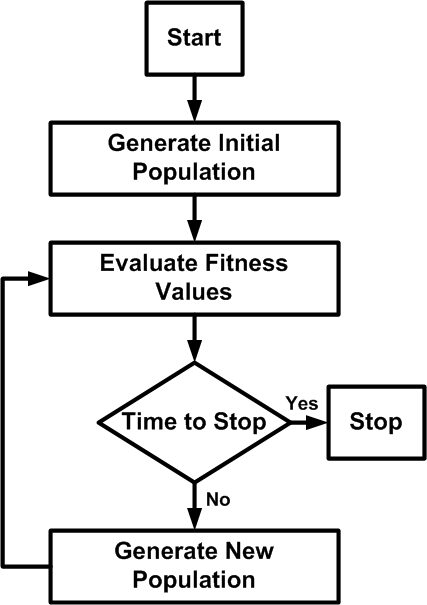
\includegraphics[keepaspectratio, width=0.2\textwidth]{EvolutionaryAlgsFC.png}}
  %\end{center}
  %\caption{\small{The general flowchart of evolutionary optimization algorithms.}}
  %\label{fig:EvolutionaryAlgsFC}
%\end{figure}

The main idea of GA is to mimic the natural selection mechanism and the survival of the fittest. In GA, the solutions are represented as chromosomes. The chromosomes are evaluated for fitness values and they are ranked from the best to the worst based on fitness value. The process to produce new solutions in GA is accomplished through three genetic operators as selection, crossover, and mutation. First, the better chromosomes are selected as parents to generate new offspring (new chromosomes). To simulate the survivor of the fittest, the chromosomes with better fitness are selected with higher probabilities. Once the parent chromosomes are selected, the crossover operator combines the chromosomes of the parents to produce new offspring (perturbation of old solutions). To avoid stagnation in the process of evolution, the mutation operator is performed on the chromosomes to increase the diversity of the population. To successfully apply the GA, the solution representation (i.e. chromosome model) must be designed carefully. Also, the parent selection process, and the probability of crossover and mutation are important parameters that must be precisely chosen \cite{Kachitvichyanuku:2012}.

In PSO, a solution is represented as a particle, and the population of solutions is called a swarm of particles. The first process in PSO is the initialization process where the initial swarm of particles is generated. Each particle is initialized with a random position and velocity. Each particle is then evaluated for fitness value. Each time a fitness value is calculated, it is compared against the previous best fitness value of the particle and the previous best fitness value of the whole swarm, and, accordingly, the personal best and global best positions are updated, appropriately. If a stopping criterion is not met, the velocity and position are updated to create a new swarm. The positions and velocities of particles are updated based on the personal best and global best positions, as well as the
old velocities. It should be noted that PSO algorithm does not require sorting of fitness values of solutions in any process. This might be a significant computational advantage over GA, especially when the population size is large \cite{Kachitvichyanuku:2012} \cite{Eberhart:2001}.
% The velocity is updated based on three components: the old velocity (inertia or momentum term), experience of an individual particle (cognitive or self learning term), and experience of the whole swarm (group or social learning term). Each term has a weight constant associated with it.
% Throughout this paper, the fitness of the solutions in our evolutionary algorithms are evaluated using the two metrics defined in Eq.(\ref{NormMetrics}) (see Section \ref{sec:SNIPERPerfEvalApp}), namely, Normalized Mean Absolute Error (NMAE) and Normalized Mean Square Error (NMSE) where $x_{ij}$ denotes the $ij^{th}$ entry of the matrix $X$ (which is known in the learning stage indicated by $T_{0}$) and $\hat{x}_{ij}$ denotes the $ij^{th}$ entry of the matrix $\hat{X}$ which is output of the MC process. 
%\begin{equation} \label{NormMetrics}
%\footnotesize{
%\begin{aligned}
%NMAE = \frac{\sum_{ij \in \bar{\Omega}} \left|x_{ij} - \hat{x}_{ij}\right|}{\sum_{ij \in \bar{\Omega}} \left|x_{ij}\right|} \\
%NMSE = \frac{\sqrt{\sum_{ij \in \bar{\Omega}} \left(x_{ij} - \hat{x}_{ij}\right)^{2} }}{\sqrt{\sum_{ij \in \bar{\Omega}} \left(x_{ij}\right)^{2}}}
%\end{aligned}
%}
%\end{equation}
Here, a solution in the GA is represented as a chromosome which is defined as a binary sampling matrix $C$ with size $n \times T_{0}$ and where $0$ and $1$ respectively represent unobserved and directly measured entries. The number of measurements paths (i.e. samples) for each chromosome is denoted by $K$ (i.e. the number of one's in each chromosome, see Section. \ref{sec:SNIPERPerfEvalApp}). To successfully apply the MC technique, the sampling matrix $C$ is constrained to have at least one $1$ in each row and column. The GA is started by generating $N_{p}$ chromosomes/solutions in the initialization step and estimating all unknown IAI in the set $\bar{\Omega}$ using MC algorithm. Then, the fitness of each chromosome is evaluated using the cost function Eq.(\ref{NormMetrics}). Accordingly, the best chromosomes, with lowest fitness values, are selected and the crossover operation, with probability $p_{c}$, is applied on each pair of parents to generate new children (offsprings). Eq.(\ref{GACrossOver}) defines the crossover operation where $r_{c}$ denotes a randomly chosen row from set $\{1,...,n\}$. These Offsprings form part of the new chromosomes of the next generation. To increase the diversity of the population, the mutation operation is performed on each child where the mutation operator changes an entry of sampling matrix $C$ from zero-to-one or vice-versa with probability $p_{m}$. The GA process is continued over $N_{i}$ iterations and the best chromosome in each iteration remains unchanged. In most cases throughout this paper, the GA parameters are set as: $N_{i}=60$, $N_{p}$=1500, $p_{c}=0.3$, and $p_{m}=0.01$.
% Among these, the best chromosome remains unchanged; and also, some simple manipulations are applied at each step to keep the number of measurement paths constant for each sampling rate in such a way that chromosomes remain symmetric (if it is required, for example, in the case of delay measurement) with having at least an one in each row/column of $C$ (please refer to \cite{SNIPERTechReport:2014} for further details). The GA process is continued over $N_{i}$ iterations.
\begin{equation} \label{GACrossOver}
% \small{
\begin{aligned}
\text{OffSpring}_{1} = C_{1}(1:r_{c},:) + C_{2}(r_{c}+1:n,:) \\
\text{OffSpring}_{2} = C_{2}(1:r_{c},:) + C_{1}(r_{c}+1:n,:) 
\end{aligned}
% }
\end{equation}

Likewise, the PSO is started by generating $N_{p}$ particles and estimating all unknown IAI in the set $\bar{\Omega}$ using the MC algorithm. The $i^{th}$ particle is identified by its position $P^{k}_{i}$ and its velocity $V^{k}_{i}$ at iteration $k$. Here, $P^{k}_{i}$ is an $n \times T_{0}$ binary matrix, representing the measurement matrix, and $V^{k}_{i}$ is also an $n \times T_{0}$ matrix. In the initialization stage all position and velocity matrices are zero matrices. The best position of $i^{th}$ particle obtained until iteration $k$ is denoted by $BP_{i}^{k}$ and the best position among all particles in the swarm until iteration $k$ is called global best position and it is denoted by $GP^{k}$. The best particles here is determined by evaluating the fitness of each particle and choosing the one with the minimum error value (as defined in Eq.(\ref{NormMetrics})) among all iterations (for one particle) or among all particles. The velocity $V^{k}_{i}$ is  updated according to Eq.(\ref{PSOPosVlc}) where $\beta_{1}$ and $\beta_{2}$ are acceleration constants, which here they setup to $\beta_{1}=\beta_{2}=2$, and $\alpha_{1}$ and $\alpha_{2}$ are standard uniform random variables in interval $[0,1]$. The positive inertia weight $\omega$ is computed as  $\omega=\omega_{max}-(\omega_{max}-\omega_{min})\frac{k}{N_{i}}$ where $\omega_{min}$ and $\omega_{max}$ are respectively minimum and maximum inertia weights which, here, we setup to $\omega_{min}=0.3$, $\omega_{max}=0.9$ and $N_{i}=2000$. The particle positions are updated (by re-determining new IAI) using two methods: 1) set the entries $\{p^{k}_{i_{kl}}\}_{kl\in I^{V}_{max}}=1$ where $I^{V}_{max}$ indicates the set of $kl^{th}$ entries with highest velocities in the matrix $V^{k}_{i}$ (i.e. $(\sim,I^{V}_{max})=sort(abs(V^{k}_{i}(:)))$), and 2) $\{p_{kl}\}$ is set to one with probability $sigmoid(v_{ij})$, where $sigmoid(x):=\frac{1}{1+e^{-x}}$, otherwise it is set to zero. The PSO process is continued for $N_{i}$ iterations.
\begin{equation} \label{PSOPosVlc}
% \footnotesize{
\begin{aligned}
V_{i}^{k} = \omega V_{i}^{k-1}+ \alpha_{1} \beta_{1} (BP_{i}^{k}-P_{i}^{k-1}) + \alpha_{2} \beta_{2} (GP^{k}-P_{i}^{k-1}) \\
\end{aligned}
% }
\end{equation}

In both GA and PSO evolutionary algorithms, simple manipulations are applied at each step to keep the number of observed IAI constant for each sampling rate in such a way that chromosomes/particles remain symmetric (if it is required, e.g., in the case of delay measurement) with having at least an one in each row and column of the solution representation.
% % (please refer to \cite{SNIPERTechReport:2014} for further details).
\section{SNIPER Performance Evaluation Methodology}  \label{sec:SNIPERPerfEvalApp}
The performance of SNIPER is evaluated by applying it to two main applications, namely per-flow size and per-flow delay estimations. For this purpose three network topologies, including Abilene, Geant and Harvard networks, and both synthesis and real network traces are considered. For per-flow size estimation, we use real traffic traces from Abilene \cite{Abilene} and GEANT \cite{Uhlig:2006} networks; the characteristics of these traffic traces are represented in Table \ref{tab:DataSetProp}. For per-flow path delay estimation, we first use the Abilene and Geant network topologies to generate the required synthetic data-set where it is assumed that the path delay for the flow between node $i$ and node $j$ is modeled as Eq.(\ref{DelayModel}). In this model, $d^{p}_{ij}$ is the propagation delay between $i^{th}$ and $j^{th}$ nodes, and $q_{ij}$ is the queuing delay in which ,according to \cite{Pietro:2008}, it is modeled as $q_{ij} \sim exp(\lambda)$. Since the average propagation delay in both Abilene and Geant networks is approximately 3.5 ms, thus, the range of the variation of $\lambda$ is chosen in $0 \leq \lambda \leq 10$ which includes both low and high noise scenarios. In addition, we use real per-flow delay from Harvard \cite{JLedlie:2007} which contains 2,492,546 measurements of application-level RTTs, with timestamps, between 226 Azureus clients collected in 4 hours \cite{YLiao:2011}.

% the parameter $\lambda$ is chosen such that $0 \leq q_{ij} \leq 10$
\begin{equation} \label{DelayModel}
% \small
\begin{aligned}
d_{ij}=d^{p}_{ij}+q_{ij}
\end{aligned}
% }
\end{equation}

\begin{table}[b]
	\centering
 %\small{
 %\renewcommand{\tabcolsep}{0.05cm}
 %\renewcommand{\arraystretch}{1.0}
		\begin{tabular}{| c | c | c | c | c | c |}
		\hline
     Network  & Date       & Duration  & Resolution   & TM Size ($n \times \mathcal{T}_{0}$)              \\ \hline
    \hline
      Abilene \cite{Abilene}   & 2004-05-01 &  1 week   &  5 min. & 144 $\times$ 2016    \\ \hline
      GEANT \cite{Uhlig:2006}  & 2005-01-08 &  1 week   & 15 min. & 529 $\times$ 672     \\ \hline
    \end{tabular}
		\vspace{0.15cm}
	\caption{Real Datasets under study.}
	\label{tab:DataSetProp}
%}
\end{table}

In our supervised learning scheme, each data-set is divided into $t_{p}$ parts. The first part, called learning epoch, with size $n \times T_{0}$ (where $ T_{0}=\left\lceil \frac{\mathcal{T}_{0}}{t_{p}}\right\rceil$) is utilized to design the OOM using the GA and PSO evolutionary algorithms. The last population of the learning stage determines the OOM and its estimation performance is denoted by subscript $T_{0}$ in our results. Then, the same OOM is used over other $t_{p}-1$ parts of the data-set (called measurement epochs) and the average of the performance over multiple parts is computed and is denoted by subscript $Avg$ in our results. The number of measurement paths, denoted by $K$, plays an important role in improving the estimation accuracy. This parameter is defined as $K=s.(n.T_{0})$ where $s$ is the Sampling Ratio (SR) and $0 \leq s \leq 1$.  Thus, given sampling ratio $s$ and having $n$ and $T_{0}$, consequently, $K$ (as the number of required measurements) and the amount of required resources can be computed. Note that, the higher the $K$ is, the better the estimation accuracy is.

The performance of NI methods in SNIPER framework, that is, the estimation accuracy of the completion of the matrix of IAI is evaluated using the following two criteria in Eq.(\ref{NormMetrics}) where NMAE denotes Normalized Mean Absolute Error and NMSE denotes Normalized Mean Square Error. The status of the IAI are also classified into two different classes. In the case of classifying per-flow delays, the flow delay estimates are compared with a threshold $\theta$ which is set as the average delay in the data-set. On the other hand, in the case of classifying per-flow sizes, the flow size estimates are compared with a threshold $\theta$ which is set as a fraction of the link capacity $C_{l}$; here, $C_{l}$ is set to the maximum flow size in the available data-set. Accordingly, the performance of the detection of congested paths (i.e. flows with delay longer than the threshold) and heavy hitters (i.e. flows larger than the threshold) are computed by the probability of detection $P^{d}$ and probability of false alarm $P^{fa}$ in Eq.(\ref{PdPfaCSHH}). Here, different subscripts are used to distinguish between different applications where $CP$ denotes Congested Paths and $HH$ denotes Heavy Hitters, respectively.
% Throughout this paper, the fitness of the solutions in our evolutionary algorithms are evaluated using the two metrics defined in Eq.(\ref{NormMetrics}) (see Section \ref{sec:SNIPERPerfEvalApp}), namely, Normalized Mean Absolute Error (NMAE) and Normalized Mean Square Error (NMSE) where $x_{ij}$ denotes the $ij^{th}$ entry of the matrix $X$ (which is known in the learning stage indicated by $T_{0}$) and $\hat{x}_{ij}$ denotes the $ij^{th}$ entry of the matrix $\hat{X}$ which is output of the MC process. 
% \hspace{0.15cm} \text{\&} \hspace{0.15cm}
\begin{equation} \label{NormMetrics}
%\small{
\begin{aligned}
NMAE = \frac{\sum_{ij \in \bar{\Omega}} \left|x_{ij} - \hat{x}_{ij}\right|}{\sum_{ij \in \bar{\Omega}} \left|x_{ij}\right|} \\
 NMSE = \frac{\sqrt{\sum_{ij \in \bar{\Omega}} \left(x_{ij} - \hat{x}_{ij}\right)^{2} }}{\sqrt{\sum_{ij \in \bar{\Omega}} \left(x_{ij}\right)^{2}}}
\end{aligned}
%}
\end{equation}
\begin{equation} \label{PdPfaCSHH}
%\small{
\begin{aligned}
& P^{d} = \frac{1}{\left| \bar{\Omega} \right|} \sum_{ij \in \bar{\Omega}}  Pr\left( \hat{x}_{ij} \geq \theta | x_{ij} \geq \theta \right) \\
& P^{fa} = \frac{1}{\left| \bar{\Omega} \right|} \sum_{ij \in \bar{\Omega}} Pr\left( \hat{x}_{ij} \geq \theta | x_{ij} < \theta \right) \\
\end{aligned}
%}
\end{equation}
\section{The Applications of SNIPER Framework} \label{sec:SNIPERResults}
In this section, we showcase the effectiveness of SNIPER for two main applications, namely per-flow delay and per-flow size estimations, and under different configurations. Each configuration determines the network under study, the matrix completion technique, the length of learning period $T_{0}$, and the sampling ratio $s$. Here, $T_{0}$ is set to $T_{0}=100$; however, $s$ mainly varies in the range of small values to indicate a case of hard constraint of network measurement resources. Other parameters, such as the number of measurement paths $K$ and the number of parts in the data-set $t_{p}$ can be determined, accordingly. The type of sampling strategies are denoted by RS, GA and PSO which respectively identify the OOM designed by Random Sampling (RS) and evolutionary algorithms GA or PSO. Note that, the performance of RS strategy is evaluated using Monte-Carlo simulation with 100 iterations.

\subsection{Optimal Observation Matrix Design using SNIPER}
The optimal design of large-scale binary observation matrices, using mathematical optimization techniques are extremely complicated or computationally expensive. Here, to show the effectiveness of our evolutionary OOM design, we consider a small ring network consisting of 4 nodes with different per-flow path delays where we can compute all possible observation matrices at a specific sampling ratio. Then, we estimate the unobserved entries and compute the corresponding $NMSE$ for all possible observation matrices. Using this process we realized that our EOAs are able to obtain the OOM. As an example, if $X=[0,5.05,9.01,9.645;5.05,0,3.96,9.645;9.01,3.96,0,5.23; \\ 4.595,9.645,5.23,0]$ (in ms) and $s=0.25$, then the optimal observation matrix $S_{\Omega}^{Opt}(X)$ with $NMSE=0.4734$ is $S_{\Omega}^{Opt}(X)=[0,0,1,0;0,0,0,1;1,0,0,0;0,1,0,0]$ which is also obtained by our GA in SNIPER framework.
%
%Here, we first show that our evolutionary OOM design procedure is able to converge to the global optimal solution. For this purpose, we consider a a small ring network consisting of 4 nodes with different per-flow path delays where we can compute all possible observation matrices at a specific sampling ratio. By estimating the unobserved entries and computing the corresponding NMSE for all possible observation matrices we realized that our OOM procedure can obtain the OOM. As an example, if $X=[0,5.05,9.01,9.645;5.05,0,3.96,9.645;9.01,3.96,0,5.23; \\ 4.595,9.645,5.23,0]$ (in ms) and $s=0.25$, then the OOM $S_{\Omega}^{Opt}(X)$ with $NMSE=0.4734$ is $S_{\Omega}^{Opt}(X)=[0,0,1,0;0,0,0,1;1,0,0,0;0,1,0,0]$ which is also obtained by our GA in SNIPER framework.

\subsection{Per-Flow Delay Estimation using SNIPER}
Figures \ref{fig:AbileneGADelayNoise} and \ref{fig:GeantGADelayNoise} show the performance of the SNIPER in the estimation of per-flow delay on Abilene and Geant networks using synthesis data generated using the model in Eq.(\ref{DelayModel}) where the MC technique is DMFSGD as in \cite{YLiao:2011}. Here, the OOM is designed using the GA and only by considering the propagation delay in Eq.(\ref{DelayModel}) in the learning epoch. Then, this OOM is used to evaluate the performance of the MC technique in measurement epochs, based on the $NMSE_{Avg}$, where queuing delay is added to the propagation delay as Eq.(\ref{DelayModel}) models the network paths delay \cite{Pietro:2008}. These two figures show that at low SRs, indicating the hard resource constraint regime, the OOM designed by the GA can obtain a better estimation accuracy, with more robust performance against noise.

Figure \ref{fig:HarvardGADelayNoise} also shows the performance of the SNIPER framework on real per-flow delay from Harvard network \cite{JLedlie:2007}. In addition, Table \ref{tab:PdfaHarvard} indicates the capability of the SNIPER framework in the reliable detection of congested paths with high probability of detection $P^{d}_{CP}$ and low probability of false alarm $P^{fa}_{CP}$. It is clear that, by increasing SR the accuracy of estimation is improved. However, at lower SRs which indicates the hard resource constraint regime, SNIPER can obtain a better estimation accuracy and more reliable detection performance, due to the intelligent design of the OOM. For example, by measuring 8.8\% of per-flow path delays, congested paths can be detected by probability 0.94 in Harvard network. This is an important factor in active network performance measurement where the network monitoring bandwidth is very limited.

It should be noted that, in Figures \ref{fig:AbileneGADelayNoise}-\ref{fig:HarvardGADelayNoise}, and throughout this paper, the blue squares represent the minimum and maximum of $NMSE$ (or $NMAE$) for each sampling ratio using our EOA based sampling strategy. Note that, in low sampling ratios and in all measurement epochs a better estimation accuracy is obtained comparing with random sampling strategy. 

% (equivalent results were obtained for Geant network)
% Comparing with the random sampling, this figure show that for lower SRs, the ONMP designed by the GA provides better estimation accuracy. Also it is more robust against the variance of the queuing delay. This is an important factor for active network measurements under hard resource constraints. 
\begin{figure*} % 30  33
  \begin{center}
\minipage{0.21\textwidth}
  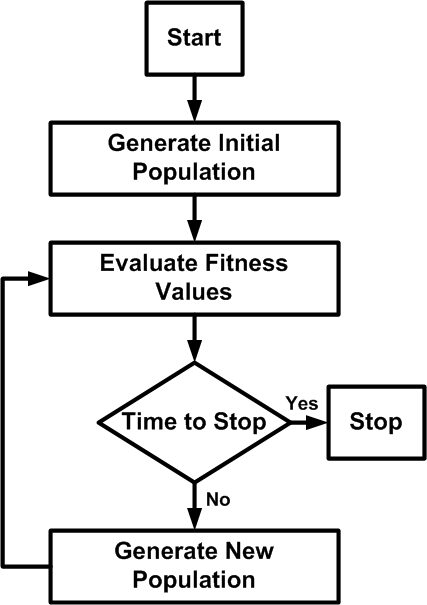
\includegraphics[width=\linewidth]{EvolutionaryAlgsFC.png}
  \caption{{The flowchart of evolutionary optimization algorithms.}}\label{fig:EvolutionaryAlgsFC}
\endminipage\hfill
\minipage{0.36\textwidth}
  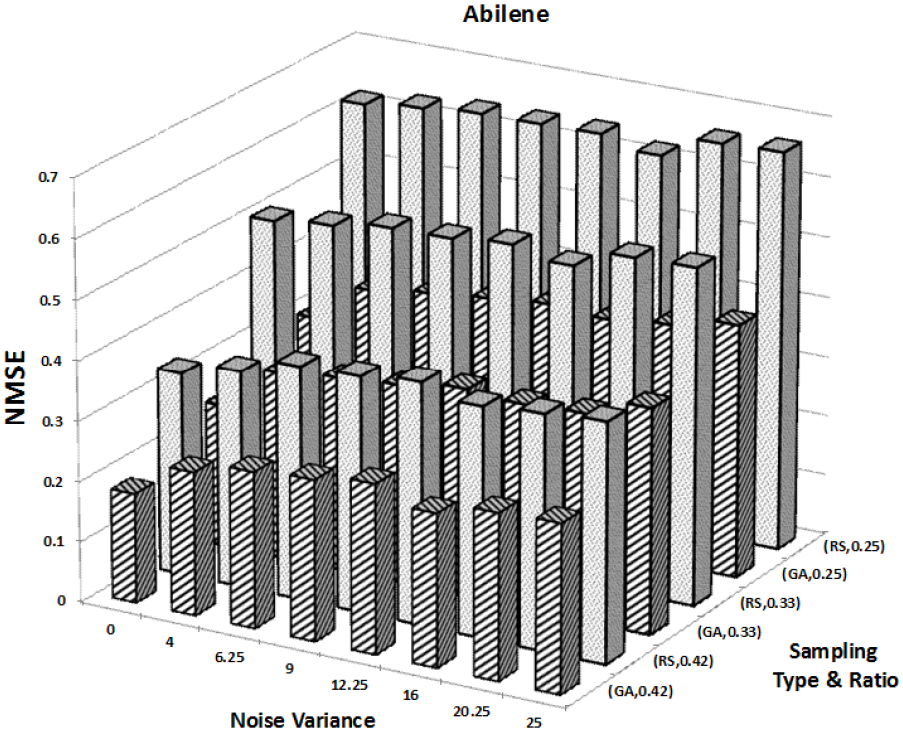
\includegraphics[width=\linewidth]{AbileneDelayNoise1.png} \hfill
  \caption{{The $NMSE$ vs. SR \& noise for Abilene.}} \label{fig:AbileneGADelayNoise}
\endminipage\hfill
\minipage{0.40\textwidth}
  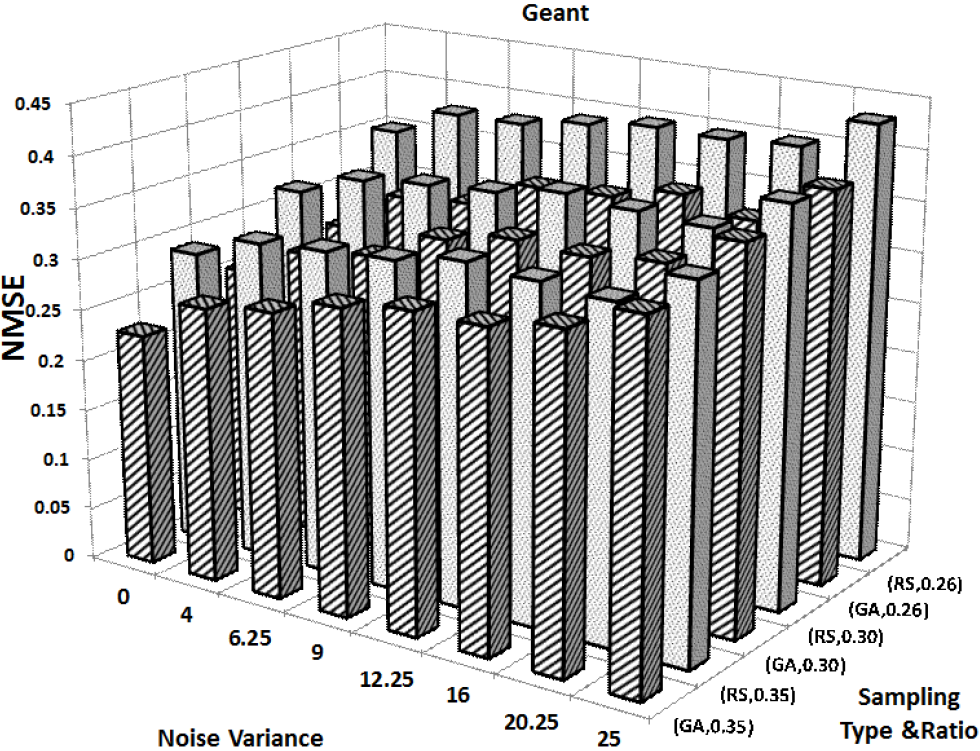
\includegraphics[width=\linewidth]{GeantDelayNoise1.png}
  \caption{{The $NMSE$ vs. SR \& noise for Geant.}} \label{fig:GeantGADelayNoise}
\endminipage
\end{center}
\end{figure*}
%\begin{figure}
  %\begin{center}
    %{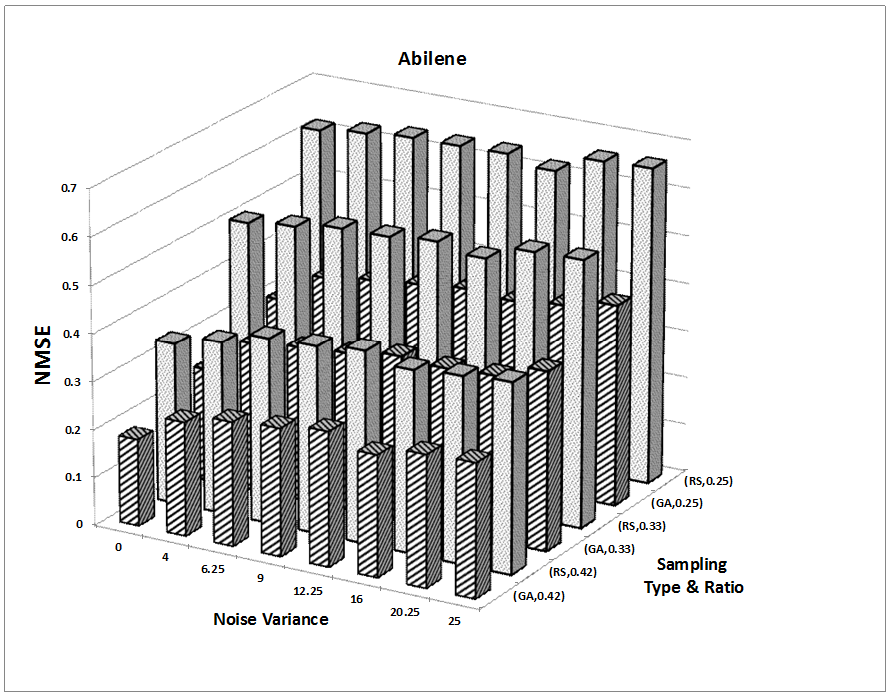
\includegraphics[keepaspectratio, width=0.49\textwidth]{AbileneDelayNoise.png}} % \\
    %{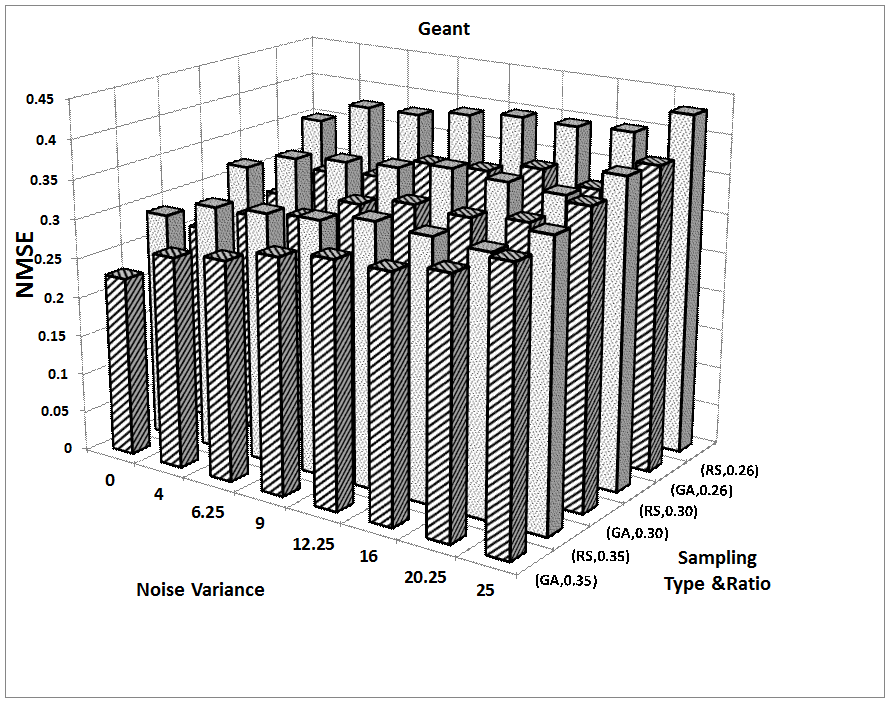
\includegraphics[keepaspectratio, width=0.49\textwidth]{GeantDelayNoise.png}}
  %\end{center}
  %\caption{{\footnotesize{The average $NMSE$ for different sampling types and ratios, and variances of queuing delay.}}}
  %\label{fig:AbileneGeantGADelayNoise}
%\end{figure}

\begin{figure}
  \begin{center}
    {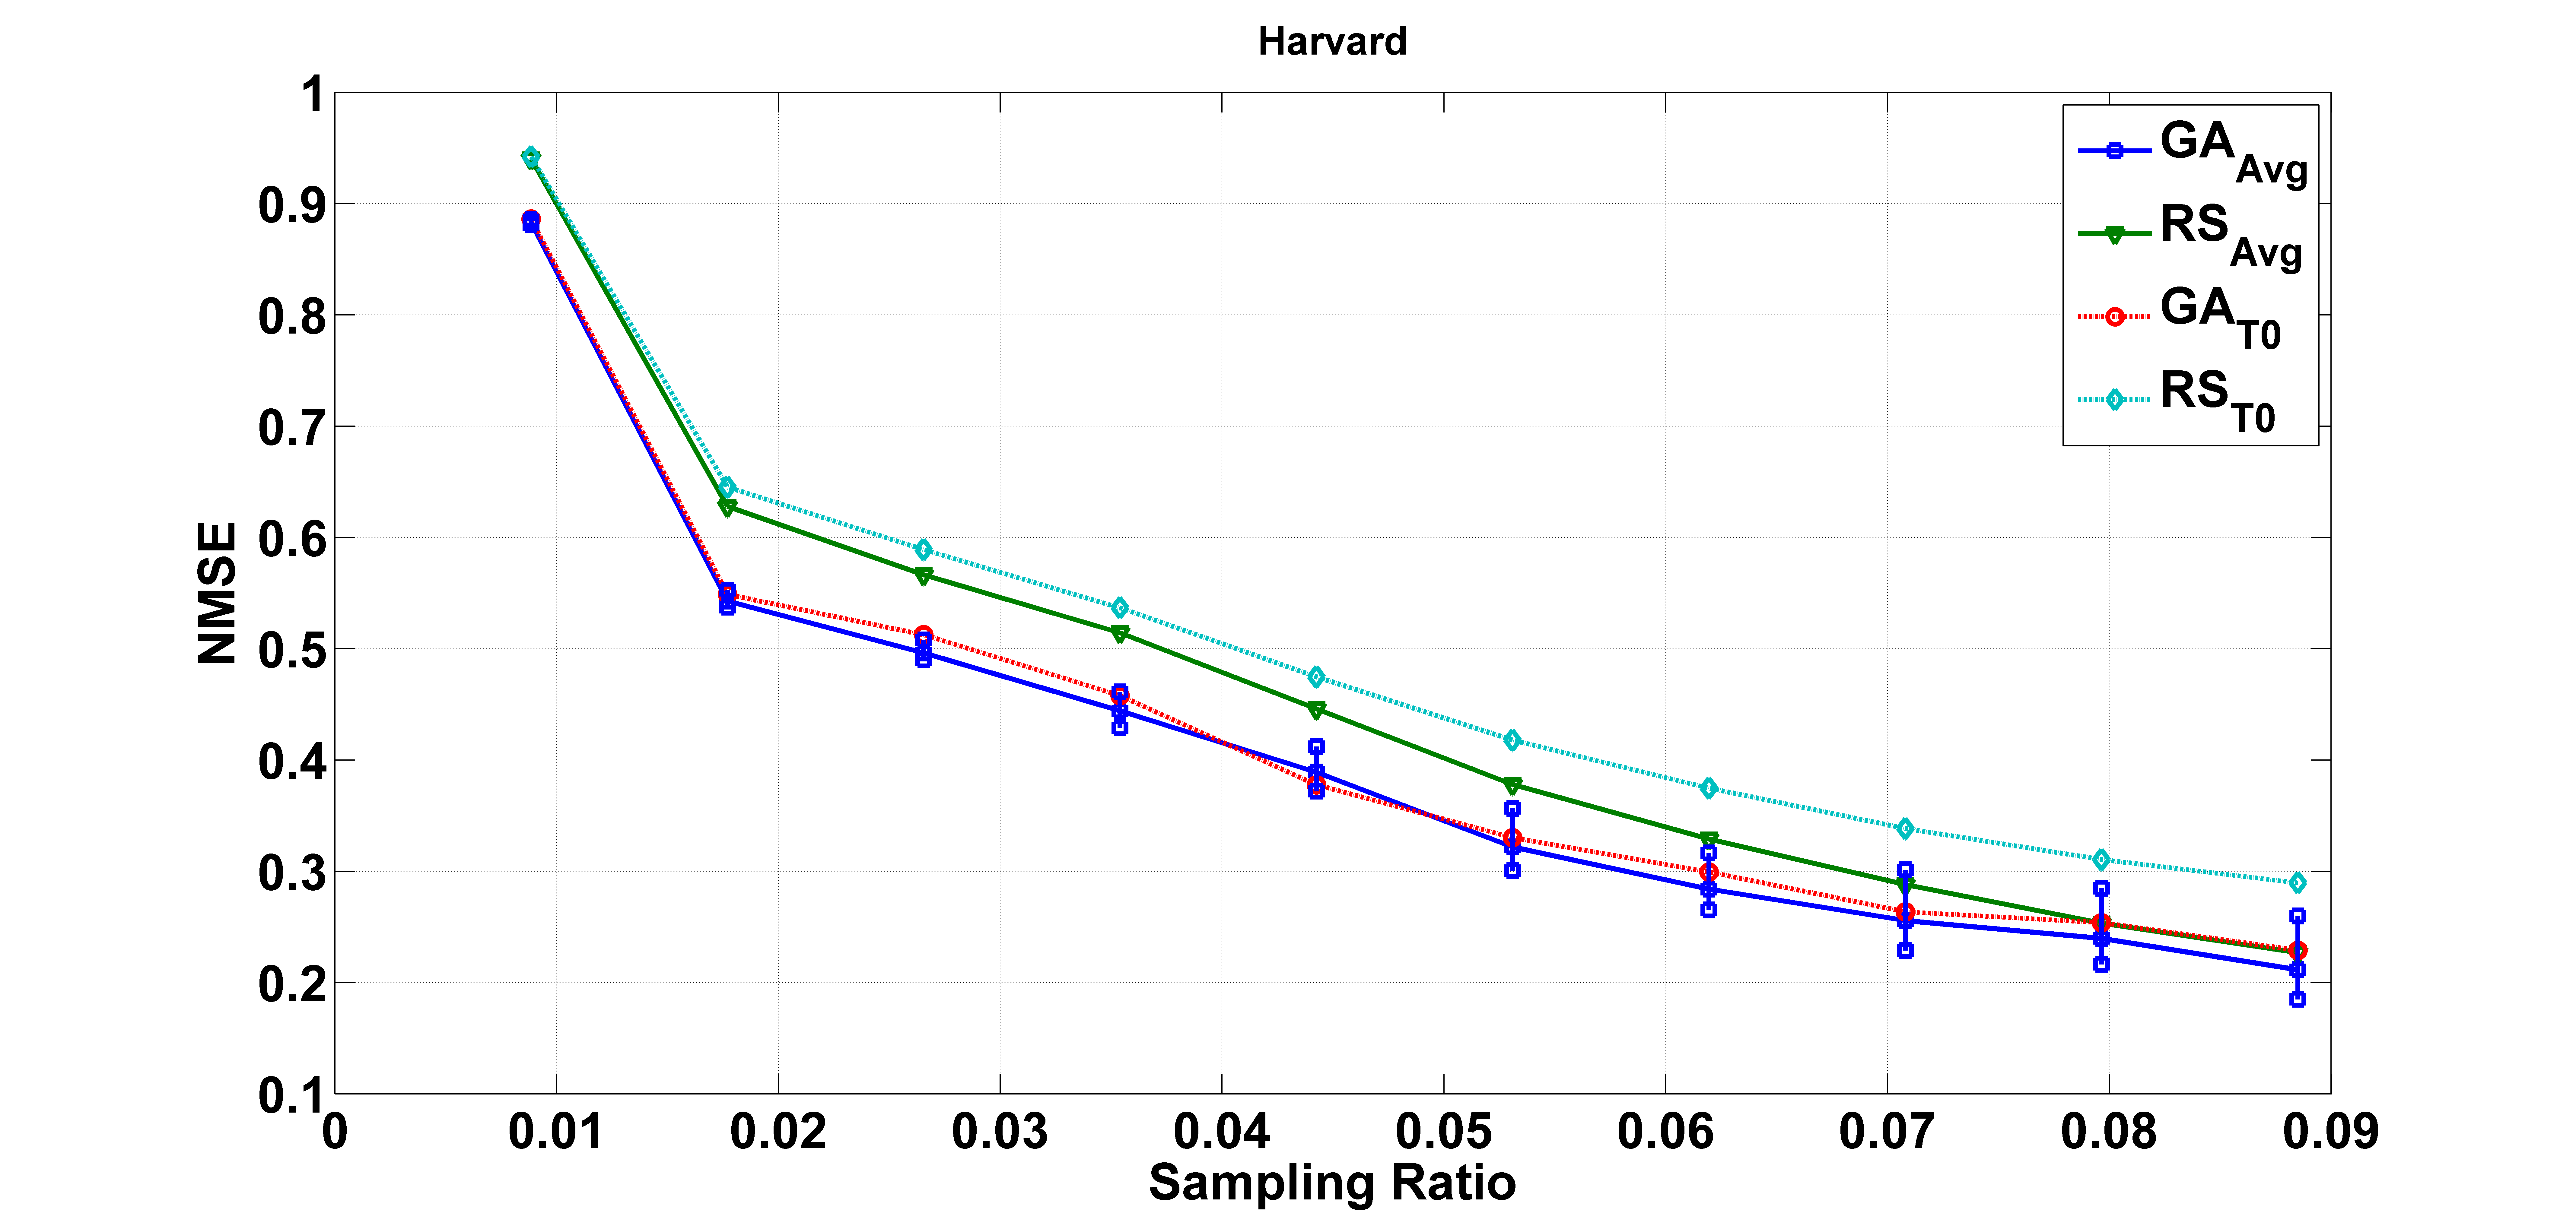
\includegraphics[keepaspectratio, width=0.49\textwidth]{HarvardGADelay.png}}
  \caption{{{The $NMSE$ for Harvard network in different sampling ratios.}}}
  \label{fig:HarvardGADelayNoise}
  \end{center}
\end{figure}

\begin{table}
	\centering
%  \footnotesize{
 %\small{
 % \renewcommand{\tabcolsep}{0.05cm}
 % \renewcommand{\arraystretch}{1.0}
		\begin{tabular}{| c | c | c | c | c | c |}
		\hline
       $SR$           &    0.0177  &  0.0354  &  0.0531  &  0.0708  &  0.0885  \\ \hline
      $P^{d}_{CP}$    &    0.6080  &  0.7534  &  0.8358  &  0.9061  &  0.9377  \\ \hline
      $P^{fa}_{CP}$   &    0.1620  &  0.1262  &  0.0750  &  0.0530  &  0.0398  \\ \hline
    \end{tabular}
	% \caption{\scriptsize{The average of $P^{d}_{CP}$ and $P^{fa}_{CP}$ for Harvard network in different sampling ratios.}}
	\vspace{0.15cm}
	\caption{{Average $P^{d}_{CP}$ and $P^{fa}_{CP}$ for Harvard network.}}
	\label{tab:PdfaHarvard}
%}
\end{table}
%\begin{table}
	%\centering
%%  \footnotesize{
 %\small{
 %% \renewcommand{\tabcolsep}{0.05cm}
 %% \renewcommand{\arraystretch}{1.0}
		%\begin{tabular}{| c | c | c | c | c | c |}
		%\hline
       %$SR$           &    0.0088  &  0.0265  &  0.0442  &  0.0619  &  0.0796  \\ \hline
      %$P^{d}_{CP}$    &    0.8077  &  0.9135  &  0.9306  &  0.9499  &  0.9566  \\ \hline
      %$P^{fa}_{CP}$   &    0.4749  &  0.2412  &  0.1661  &  0.1263  &  0.1032  \\ \hline
    %\end{tabular}
	%% \caption{\scriptsize{The average of $P^{d}_{CP}$ and $P^{fa}_{CP}$ for Harvard network in different sampling ratios.}}
	%\caption{\small{Average $P^{d}_{CP}$ and $P^{fa}_{CP}$ for Harvard network.}}
	%\label{tab:PdfaHarvard}
%}
%\end{table}

\subsection{Per-Flow Size Estimation using SNIPER}
Figure \ref{fig:AbileneGeantGATMC} shows the performance of the SNIPER in the estimation of per-flow sizes on both Abilene and Geant networks using real traffic traces (see Table \ref{tab:DataSetProp}) where the MC technique is the SRSVD-base as in \cite{Roughan:2012}. Again, it is clear that by increasing SR the accuracy of estimation is enhanced. Also, by the optimal design of observation matrix using our proposed EOA in the SNIPER framework, the performance of the matrix completion is improved, particularly at low sampling ratios which indicates the hard resource constraint of TCAM entries as the main resource for per-flow size measurement. The better accuracy is obtained almost for all sampling ratios and in all measurement epochs. Table \ref{tab:SNIPERPdPfaHH} also shows the average performance of the SNIPER framework in the reliable detection of heavy hitters under low sampling ratios. For example, by measuring 20\% of the per-flow sizes, HHs can be respectively detected with probability 0.65 and 0.78 in Abilene and Geant networks, which are higher than what can be obtained using RS. This has a great implication in different applications, such as, network traffic engineering and network security.
% Therefore, comparing with random sampling strategy, this table indicates the good capability of this framework in detection HHs even under low sampling ratios.

\begin{figure}
  \begin{center}
    {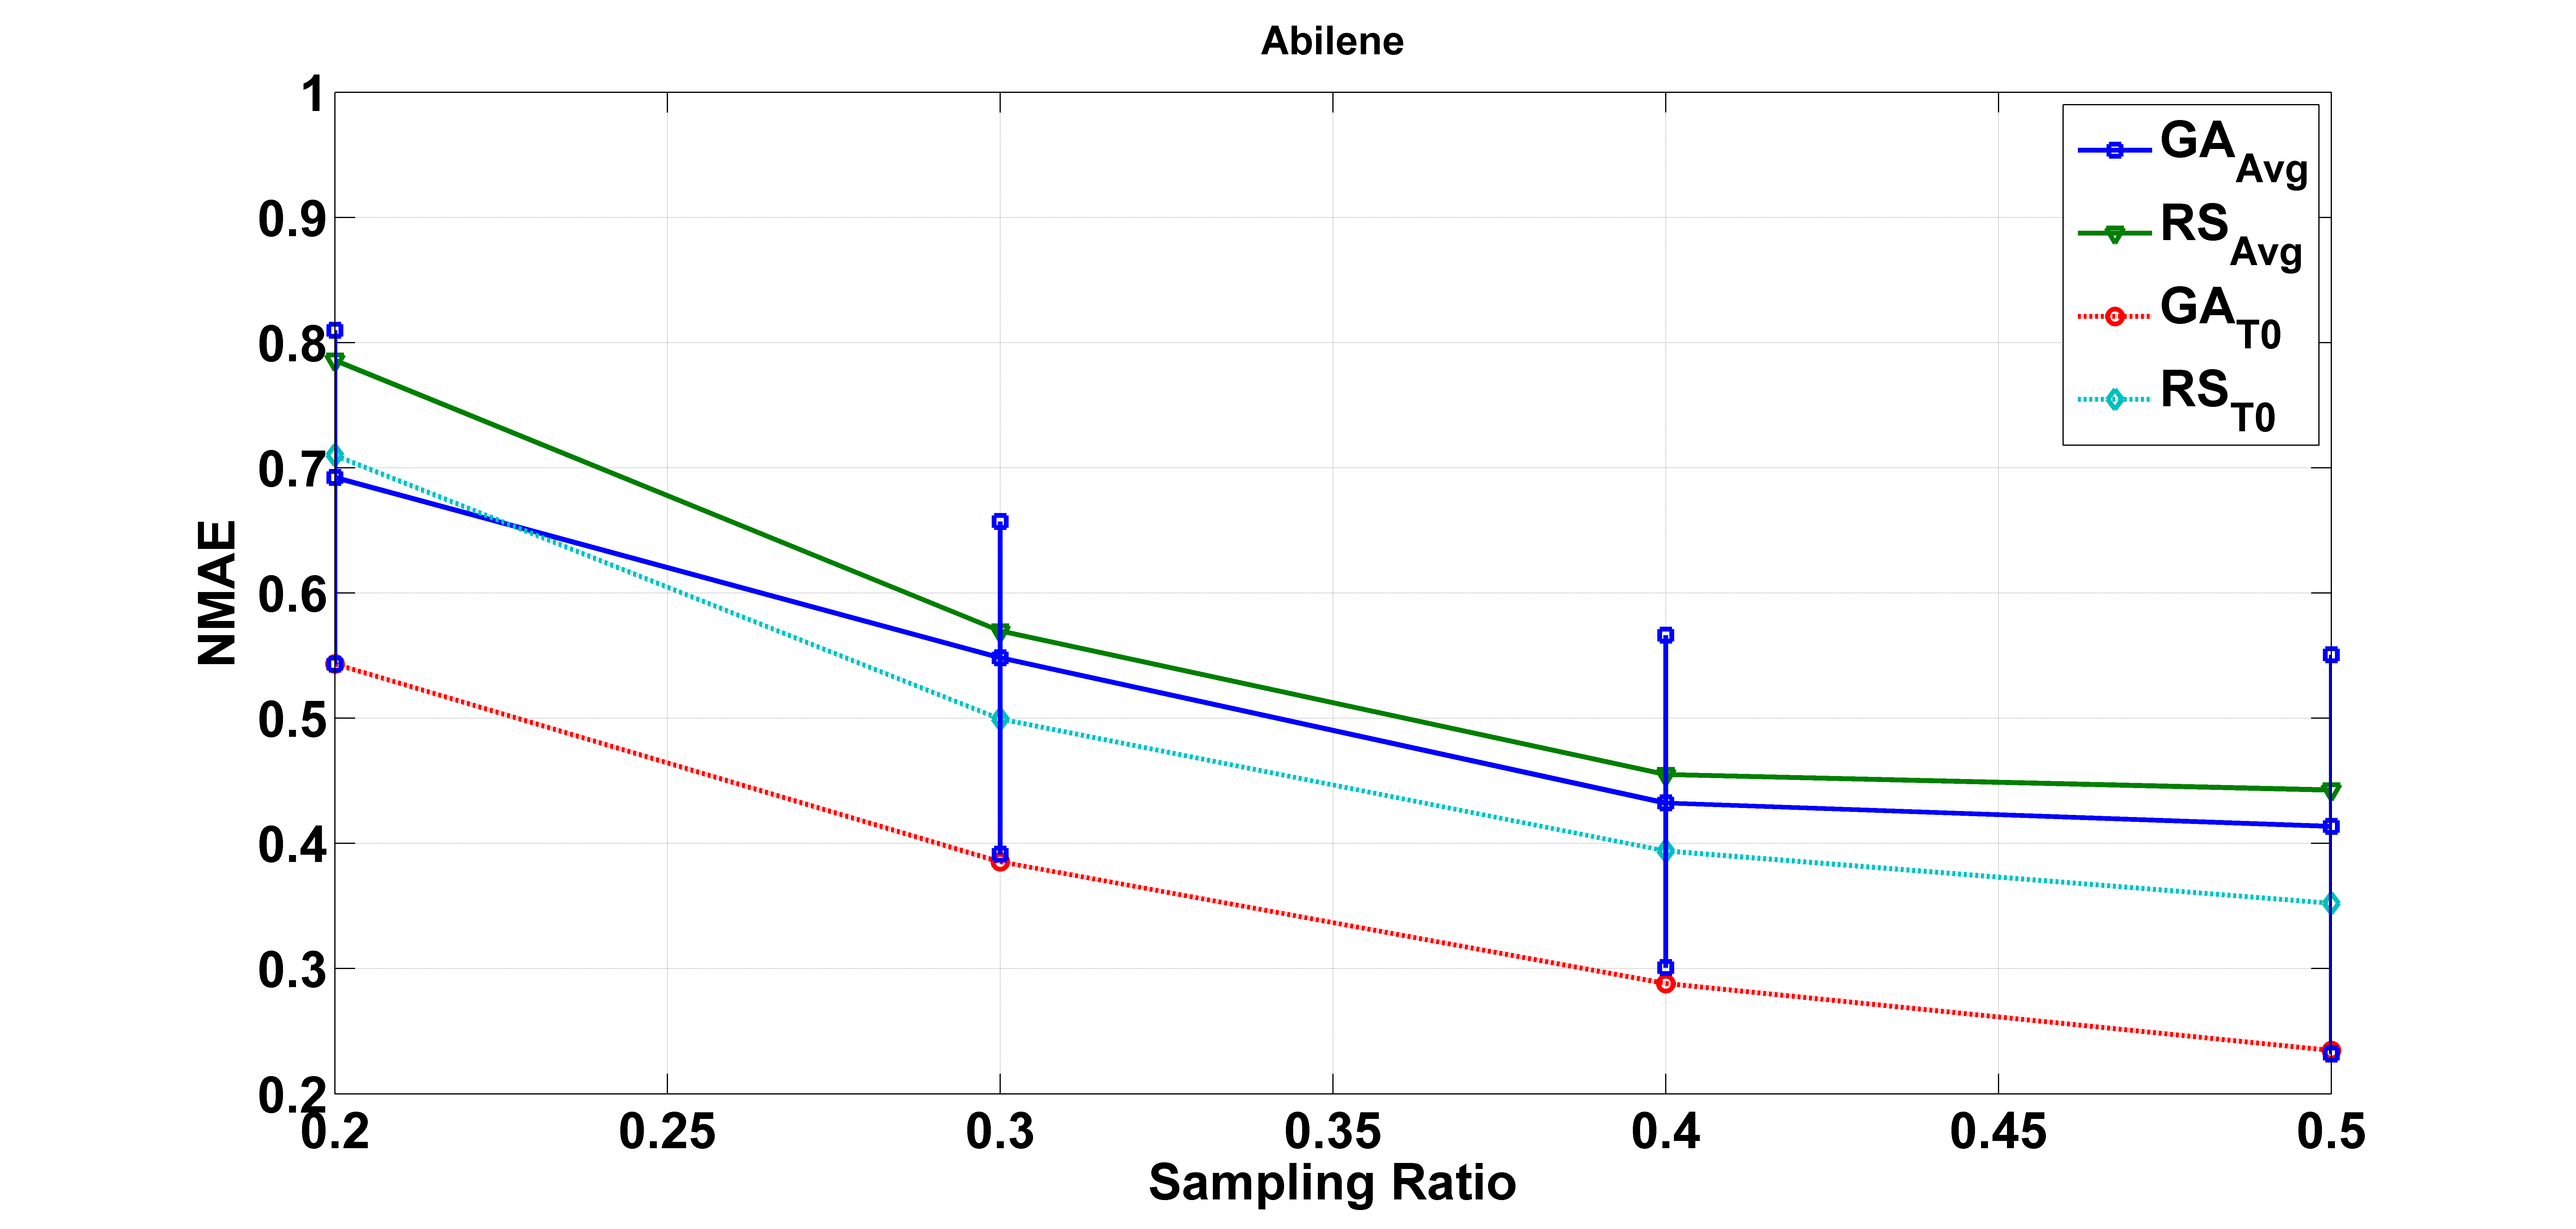
\includegraphics[keepaspectratio, width=0.49\textwidth]{AbileneGATMC.png}} \\
    {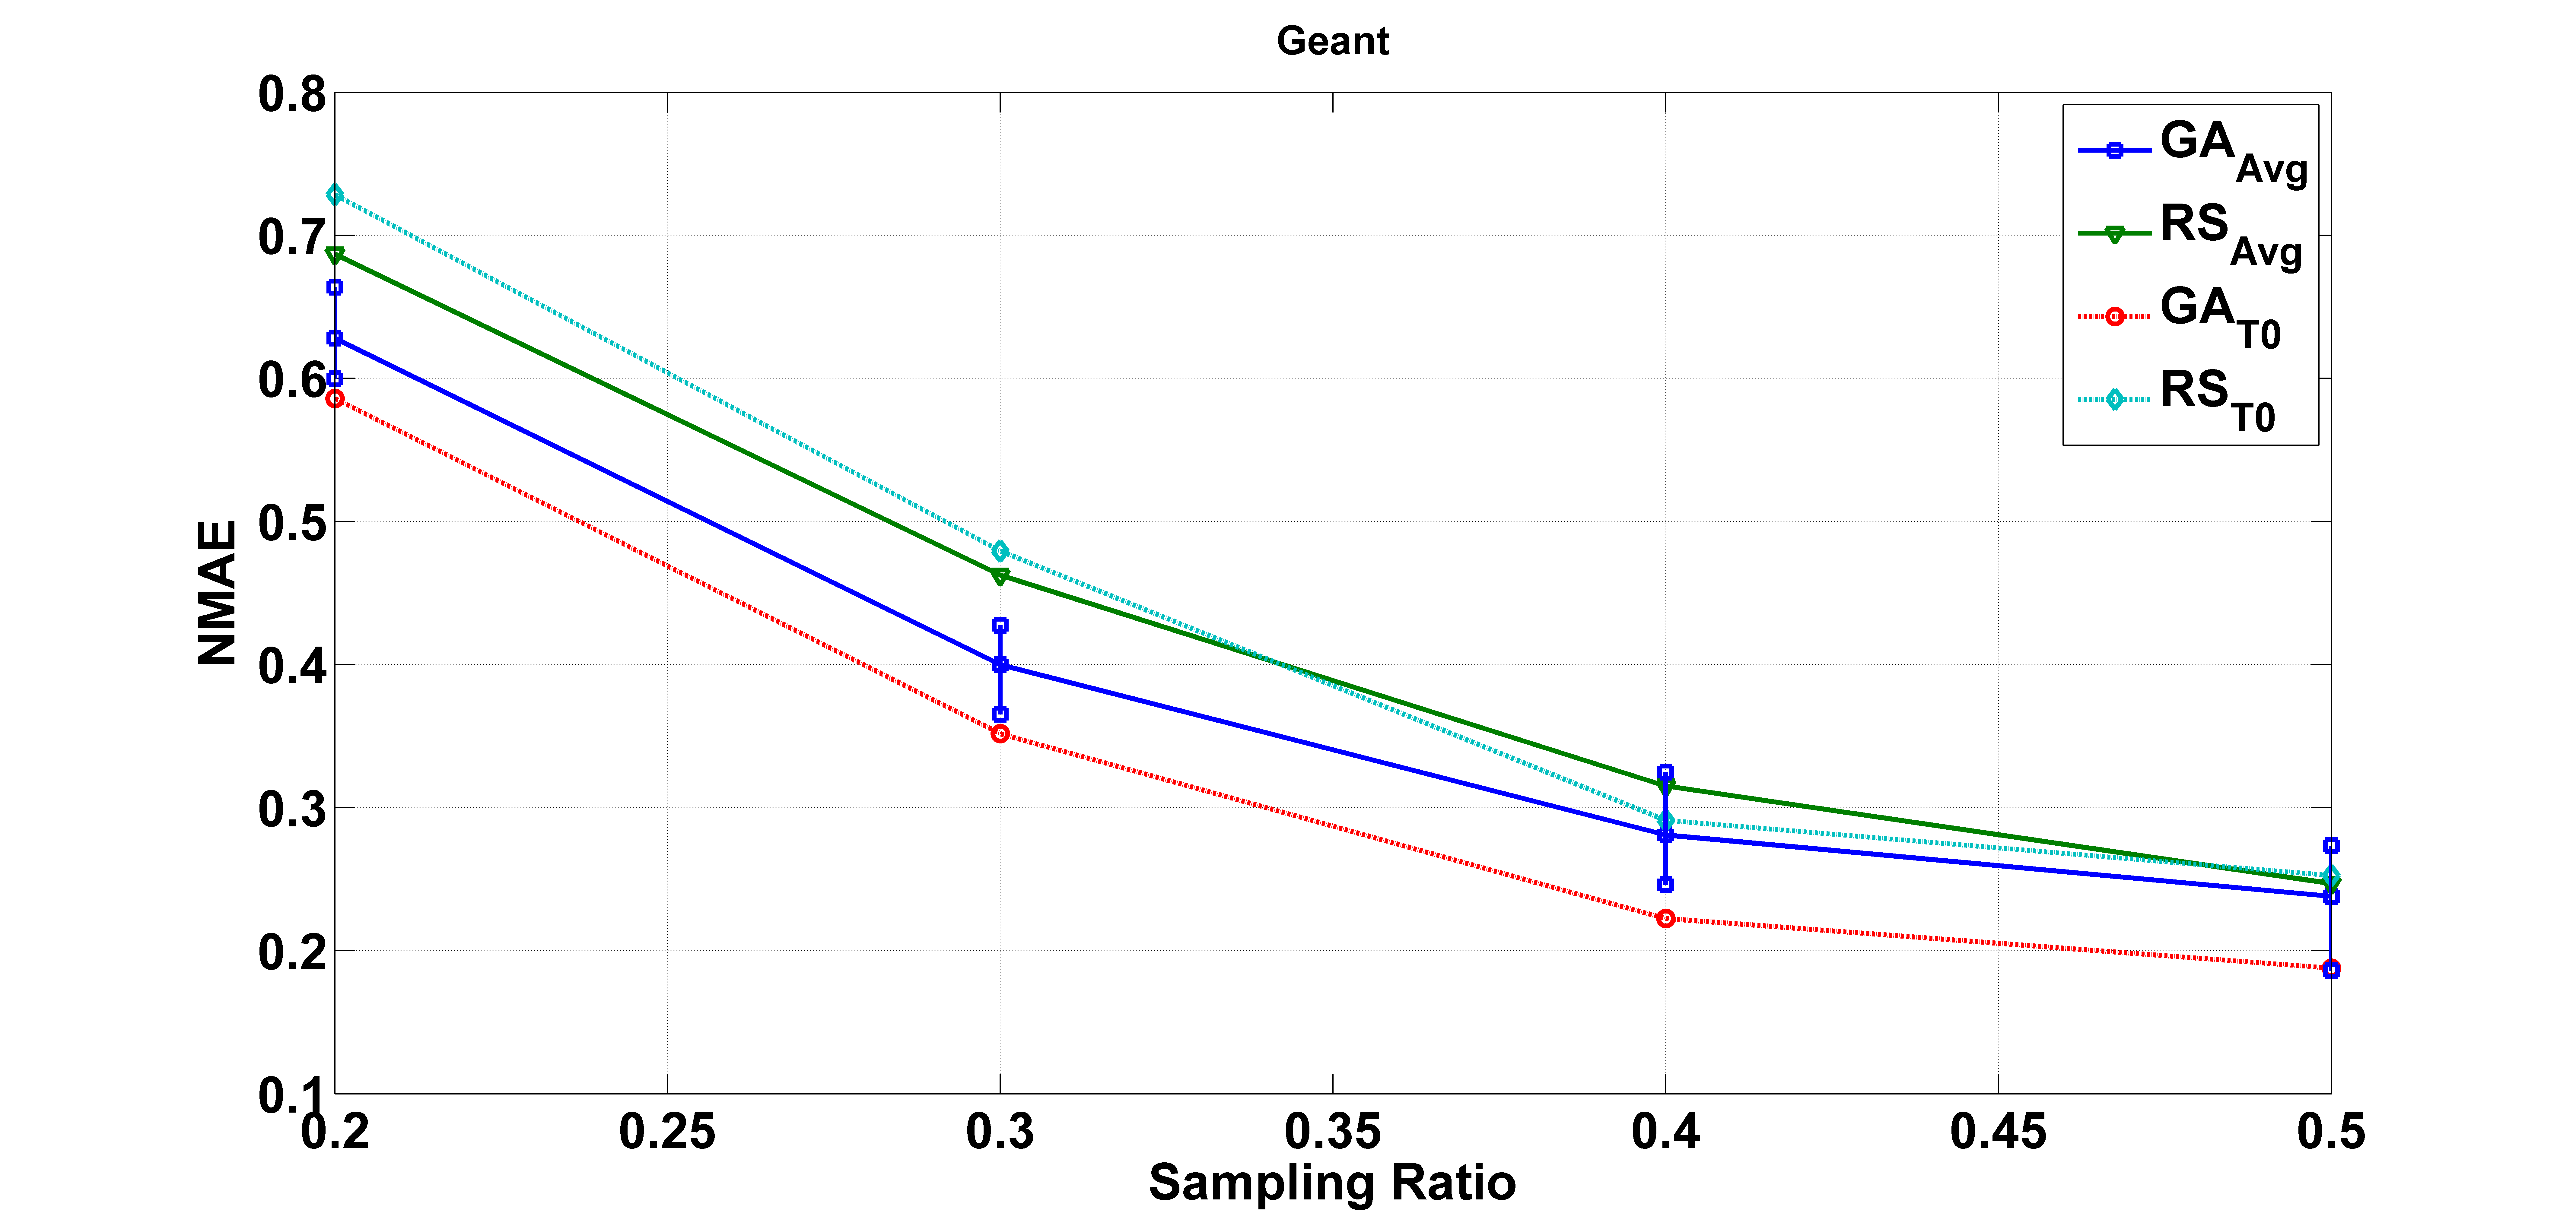
\includegraphics[keepaspectratio, width=0.49\textwidth]{GeantGATMC.png}}
  \caption{{{$NMAE$ vs. sampling ratio for Abilene and Geant networks.}}}
  \label{fig:AbileneGeantGATMC}
  \end{center}
\end{figure}

%\begin{table}
%	\centering
% \small{
% \renewcommand{\tabcolsep}{0.05cm}
% \renewcommand{\arraystretch}{1.0}
%		\begin{tabular}{| c | c | c | c | c |}
%		\hline
%                              & $SR=0.2$ & $SR=0.3$ & $SR=0.4$ & $SR=0.5$   \\ \hline
%      $P^{d}_{HH}$ (Abilene)    & 0.6550   & 0.7693   & 0.8380   & 0.8851 \\ \hline
%      $P^{fa}_{HH}$ (Abilene)   & 0.0325   & 0.0192   & 0.0142   & 0.0119 \\ \hline
%      $P^{d}_{HH}$ (Geant)      & 0.7804   & 0.9096   & 0.9375   & 0.9502 \\ \hline
%      $P^{fa}_{HH}$ (Geant)     & 0.0095   & 0.0058   & 0.0041   & 0.0034 \\ \hline
%    \end{tabular}
%	\caption{\scriptsize{The average $P^{d}_{HH}$ and $P^{fa}_{HH}$ using GA for Abilene and Geant networks where $\theta=0.05 C_{l}$ and $\theta=0.1 C_{l}$, respectively.}}
%	\label{tab:SNIPERPdPfaHH}
%}
%\end{table}

%It is worth mentioning that, these results also have important implications in other applications such as recommended systems where, to reduce the number of measurements, we can intelligently ask particular customers to rate particular products which leads to the best estimate of all or sub-set of unknowns of interest. This is of particular importance, comparing with regular MC techniques which are based on the random measurements of the higher number of attributes of interest.

\subsection{Scalability of SNIPER}
As we have seen in the previous results, the SNIPER can improve the estimation accuracy under hard resource constraint regimes. To reduce the high computational complexity of the GA in designing the optimal observation matrix in large-scale networks and increase the scalability of the SNIPER framework, here, we use the PSO evolutionary optimization algorithm (see Section \ref{sec:SNIPEREvlObsMtxDsg}) which is much faster than the GA \cite{Talib:2009}\cite{Kachitvichyanuku:2012} and it can reduce the computational complexity and processing power of the SNIPER. Figure \ref{fig:AbileneGeantPSOTMC} shows the performance of SNIPER for per-flow size estimation, representing the fact that in low sampling rates the intelligent design of the observation matrix using PSO algorithm results in a better estimation accuracy. The reduction in the computational time using the PSO algorithm is quantified using the notion of Processing Gain defined in Eq(\ref{DefPG}) where $PT_{GA}$ and $PT_{PSO}$ respectively denote the processing times for running GA and PSO algorithms. The processing gains for Abilene and Geant networks are $PG$=56\% and $PG$=65\%, respectively. 
%************* explain the norm in appendix  and say that it is under investigation ******************8
%In Appendix A we propose another method to address the scalability 

\begin{equation}\label{DefPG}
%\small{
\begin{aligned}
PG \% = 100 \times \frac{PT_{GA}-PT_{PSO}}{PT_{GA}}
\end{aligned}
%}
\end{equation}

\begin{table}
	\centering
 %\small{
 %\renewcommand{\tabcolsep}{0.05cm}
 %\renewcommand{\arraystretch}{1.0}
		\begin{tabular}{| c | c | c | c | c |}
		\hline
                                   & $SR=0.2$ & $SR=0.3$ & $SR=0.4$ & $SR=0.5$   \\ \hline
      $P^{d}_{HH}$ Abilene  (RS)   & 0.6256 & 0.7544 & 0.8426 & 0.8851 \\ \hline
      $P^{d}_{HH}$ Abilene  (GA)   & 0.6550 & 0.7693 & 0.8380 & 0.8901 \\ \hline
      $P^{fa}_{HH}$ Abilene   (RS) & 0.0353 & 0.0202 & 0.0144 & 0.0116 \\ \hline
      $P^{fa}_{HH}$ Abilene   (GA) & 0.0325 & 0.0192 & 0.0142 & 0.0119 \\ \hline
      $P^{d}_{HH}$ Geant   (RS)    & 0.7606 & 0.8935 & 0.9354 & 0.9489 \\ \hline
      $P^{d}_{HH}$ Geant   (GA)    & 0.7804 & 0.9096 & 0.9375 & 0.9502 \\ \hline
      $P^{fa}_{HH}$ Geant  (RS)    & 0.0106 & 0.0061 & 0.0043 & 0.0035 \\ \hline
      $P^{fa}_{HH}$ Geant  (GA)    & 0.0095 & 0.0058 & 0.0041 & 0.0034 \\ \hline
    \end{tabular}
%%%     \newline
%%% \vspace*{0.15cm}
%%% \newline
%		\begin{tabular}{| c | c | c | c | c |}
%		\hline
%                                   & $SR=0.2$ & $SR=0.3$ & $SR=0.4$ & $SR=0.5$   \\ \hline
%      $P^{d}_{HH}$ Geant   (RS)  \hspace{0.15cm}  & 0.7606 & 0.8935 & 0.9354 & 0.9489 \\ \hline
%      $P^{d}_{HH}$ Geant   (GA)  \hspace{0.15cm}  & 0.7804 & 0.9096 & 0.9375 & 0.9502 \\ \hline
%      $P^{fa}_{HH}$ Geant  (RS)  \hspace{0.15cm}  & 0.0106 & 0.0061 & 0.0043 & 0.0035 \\ \hline
%      $P^{fa}_{HH}$ Geant  (GA)  \hspace{0.15cm}  & 0.0095 & 0.0058 & 0.0041 & 0.0034 \\ \hline
%    \end{tabular}
	\vspace{0.15cm}
  	\caption{{Comparing the average $P^{d}_{HH}$ and $P^{fa}_{HH}$ between RS and GA sampling strategies for Abilene and Geant networks where $\theta=0.05 C_{l}$ and $\theta=0.1 C_{l}$, respectively.}}
	\label{tab:SNIPERPdPfaHH}
%}
\end{table}


\begin{figure}
  \begin{center}
    {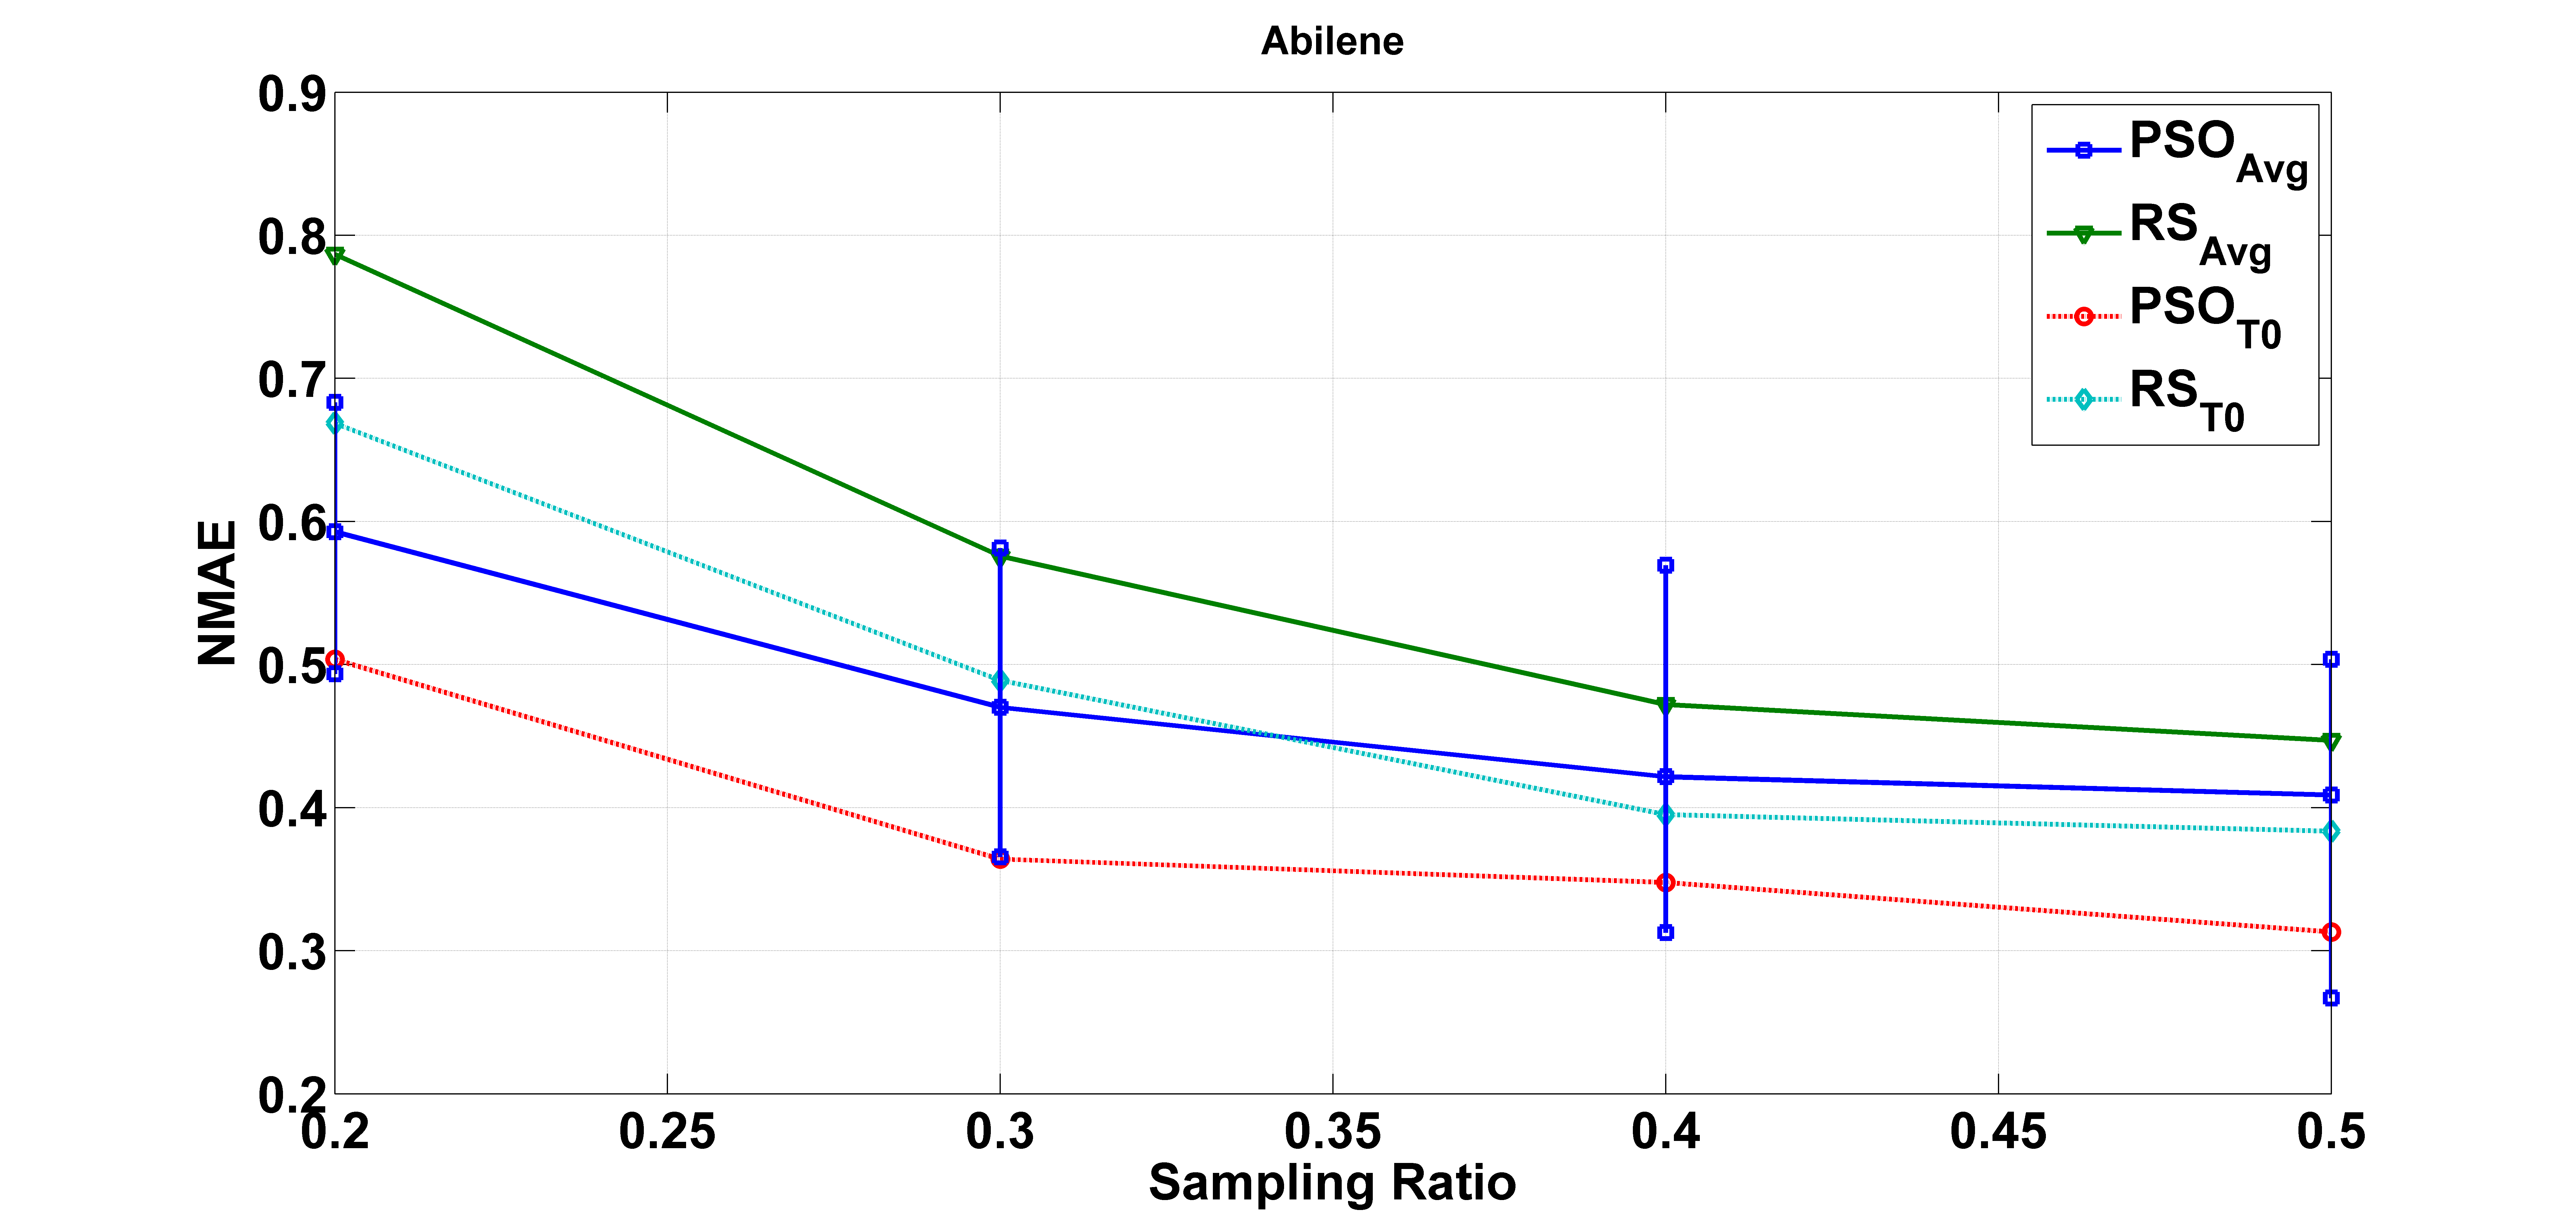
\includegraphics[keepaspectratio, width=0.49\textwidth]{AbilenePSOTMC.png}} \\
    {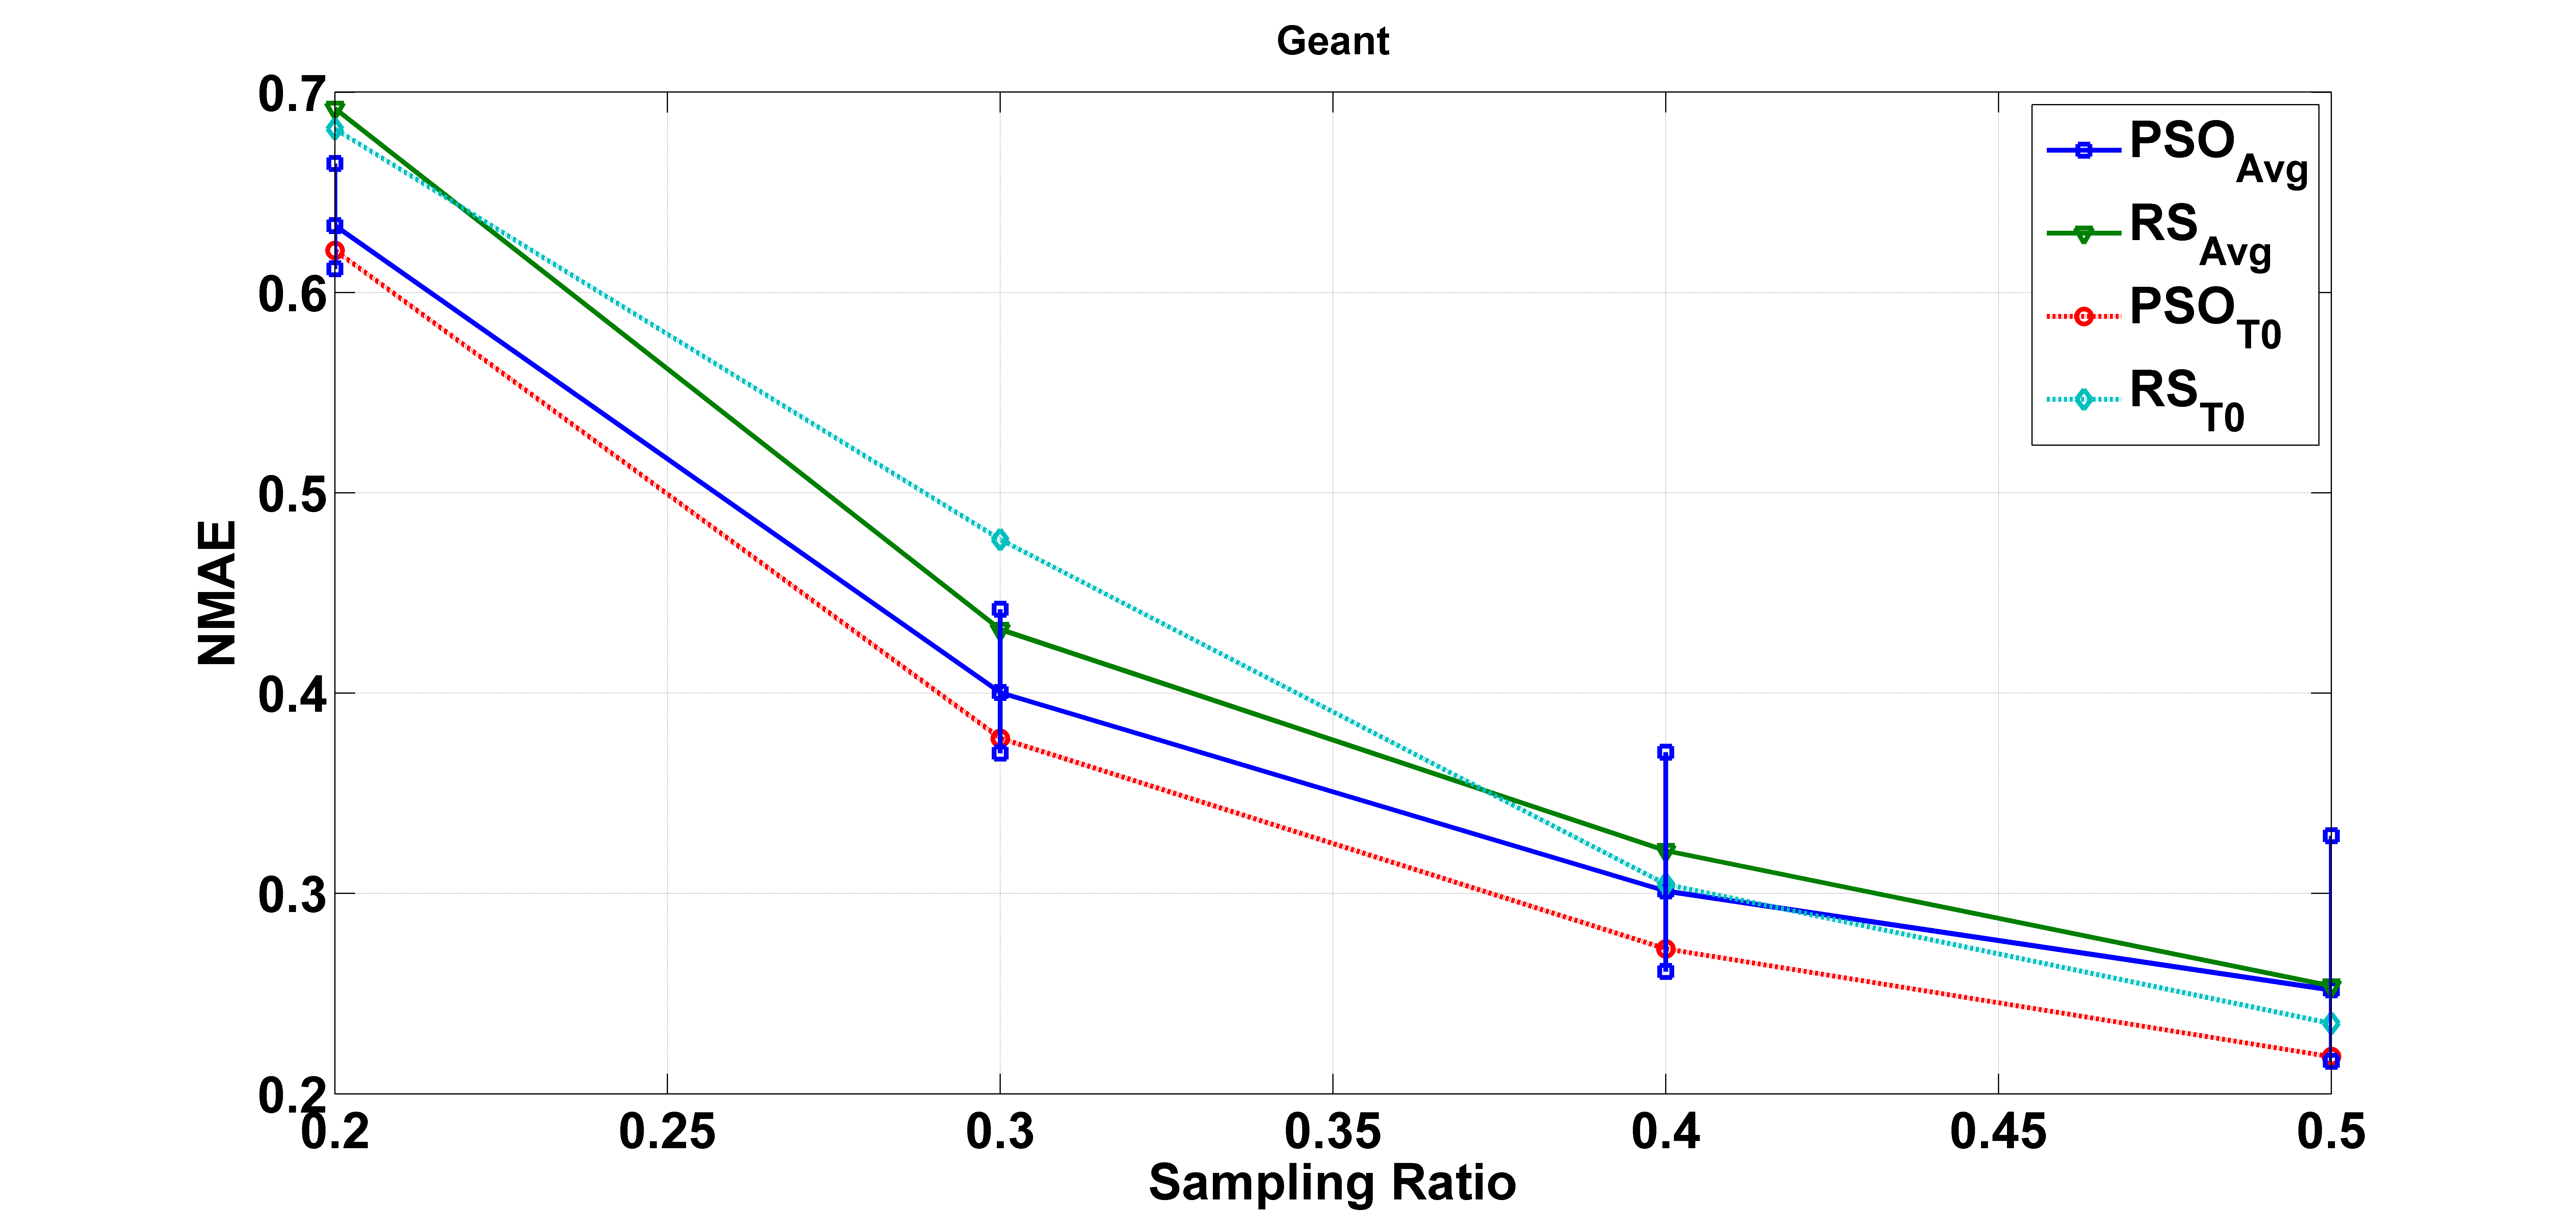
\includegraphics[keepaspectratio, width=0.49\textwidth]{GeantPSOTMC.png}}
  \caption{{{$NMAE$ vs. sampling ratio for Abilene and Geant networks.}}}
  \label{fig:AbileneGeantPSOTMC}
  \end{center}
\end{figure}
%In addition, instead of minimizing the ultimate estimation accuracy (e.g. represented by $NMAE$), the norm of the observation matrix $\Omega$  is minimized where the norm of a matrix is defined as the maximum singular value of the matrix and denoted by $sigma_{1}(\Omega)$. Note that, the norm of the observation matrix is strongly correlated with $NMAE$; this fact has been justified in Figure \ref{fig:NMAENormCorrFig} and Table \ref{tab:NMAENormCorrTab}. Also, Tables \ref{tab:FitFuncCmp1} and \ref{tab:FitFuncCmp2} shows the NMAE and the processing gains (indicated by the Time Gain) achieved by minimizing the norm of the observation matrix using both GA and PSO algorithms. Due to some inconsistency in  Table \ref{tab:FitFuncCmp1} this paragraph and its results are removed; in fact, we can conclude that to achieve a better accuracy the ultimate performance metric must be optimized.
%\begin{table}
%	\centering
% \footnotesize{
% \renewcommand{\tabcolsep}{0.05cm}
% \renewcommand{\arraystretch}{1.0}
%		\begin{tabular}{| c | c | c | c | c | c | c | c |}
%		\hline
%       Net./Prm. & $SR$ & $RS_{T_{0}}$ & $GA_{T_{0}}$ & $PSO_{T_{0}}$ & $RS^{\sigma}_{T_{0}}$ & $GA^{\sigma}_{T_{0}}$ & $PSO^{\sigma}_{T_{0}}$  \\ \hline
%      Abilene    & 0.3 & 0.499312 & 0.364073 & 0.387655 & 0.498732 & 0.503375 & 0.480801 \\ \hline
%      GEANT      & 0.2 & 0.728394 & 0.55408 & 0.60432 & 0.722275 & 0.679437 & 0.684696 \\ \hline
%    \end{tabular}
%    \newline
%\vspace*{0.15cm}
%\newline
%		\begin{tabular}{| c | c | c | c | c | c | c | c |}
%		\hline
%       Net./Prm. & $SR$ & $RS_{Avg}$ & $GA_{Avg}$ & $PSO_{Avg}$ & $RS^{\sigma}_{Avg}$ & $GA^{\sigma}_{Avg}$ & $PSO^{\sigma}_{Avg}$  \\ \hline
%      Abilene    & 0.3 & 0.569638 & 0.556108 & 0.494916 & 0.582961 & 0.546438 & 0.586098  \\ \hline
%      GEANT      & 0.2 & 0.686854 & 0.601478 & 0.644993 & 0.69442 & 0.664646 & 0.681144  \\ \hline
%    \end{tabular}
%	\caption{\scriptsize{NMAE comparison between different evolutionary fitness functions ($\sigma$ denotes norm function).}}
%	\label{tab:FitFuncCmp1}
%}
%\end{table}
%
%\begin{table}
%	\centering
% \footnotesize{
% \renewcommand{\tabcolsep}{0.05cm}
% \renewcommand{\arraystretch}{1.0}
%		\begin{tabular}{| c | c | c | c |}
%		\hline
%       Net./TimeGain & $SR$ & $Time Gain^{\sigma}_{GA}$ & $Time Gain^{sigma}_{PSO}$ \\ \hline
%      Abilene    & 0.3 & 0.937689 & 0.818912  \\ \hline
%      GEANT      & 0.2 & 0.884593 & 0.773611  \\ \hline
%    \end{tabular}
%	\caption{\scriptsize{Time Gain comparison between different evolutionary fitness functions ($\sigma$ denotes norm function).}}
%	\label{tab:FitFuncCmp2}
%}
%\end{table}
%\begin{figure}
%  \begin{center}
%    {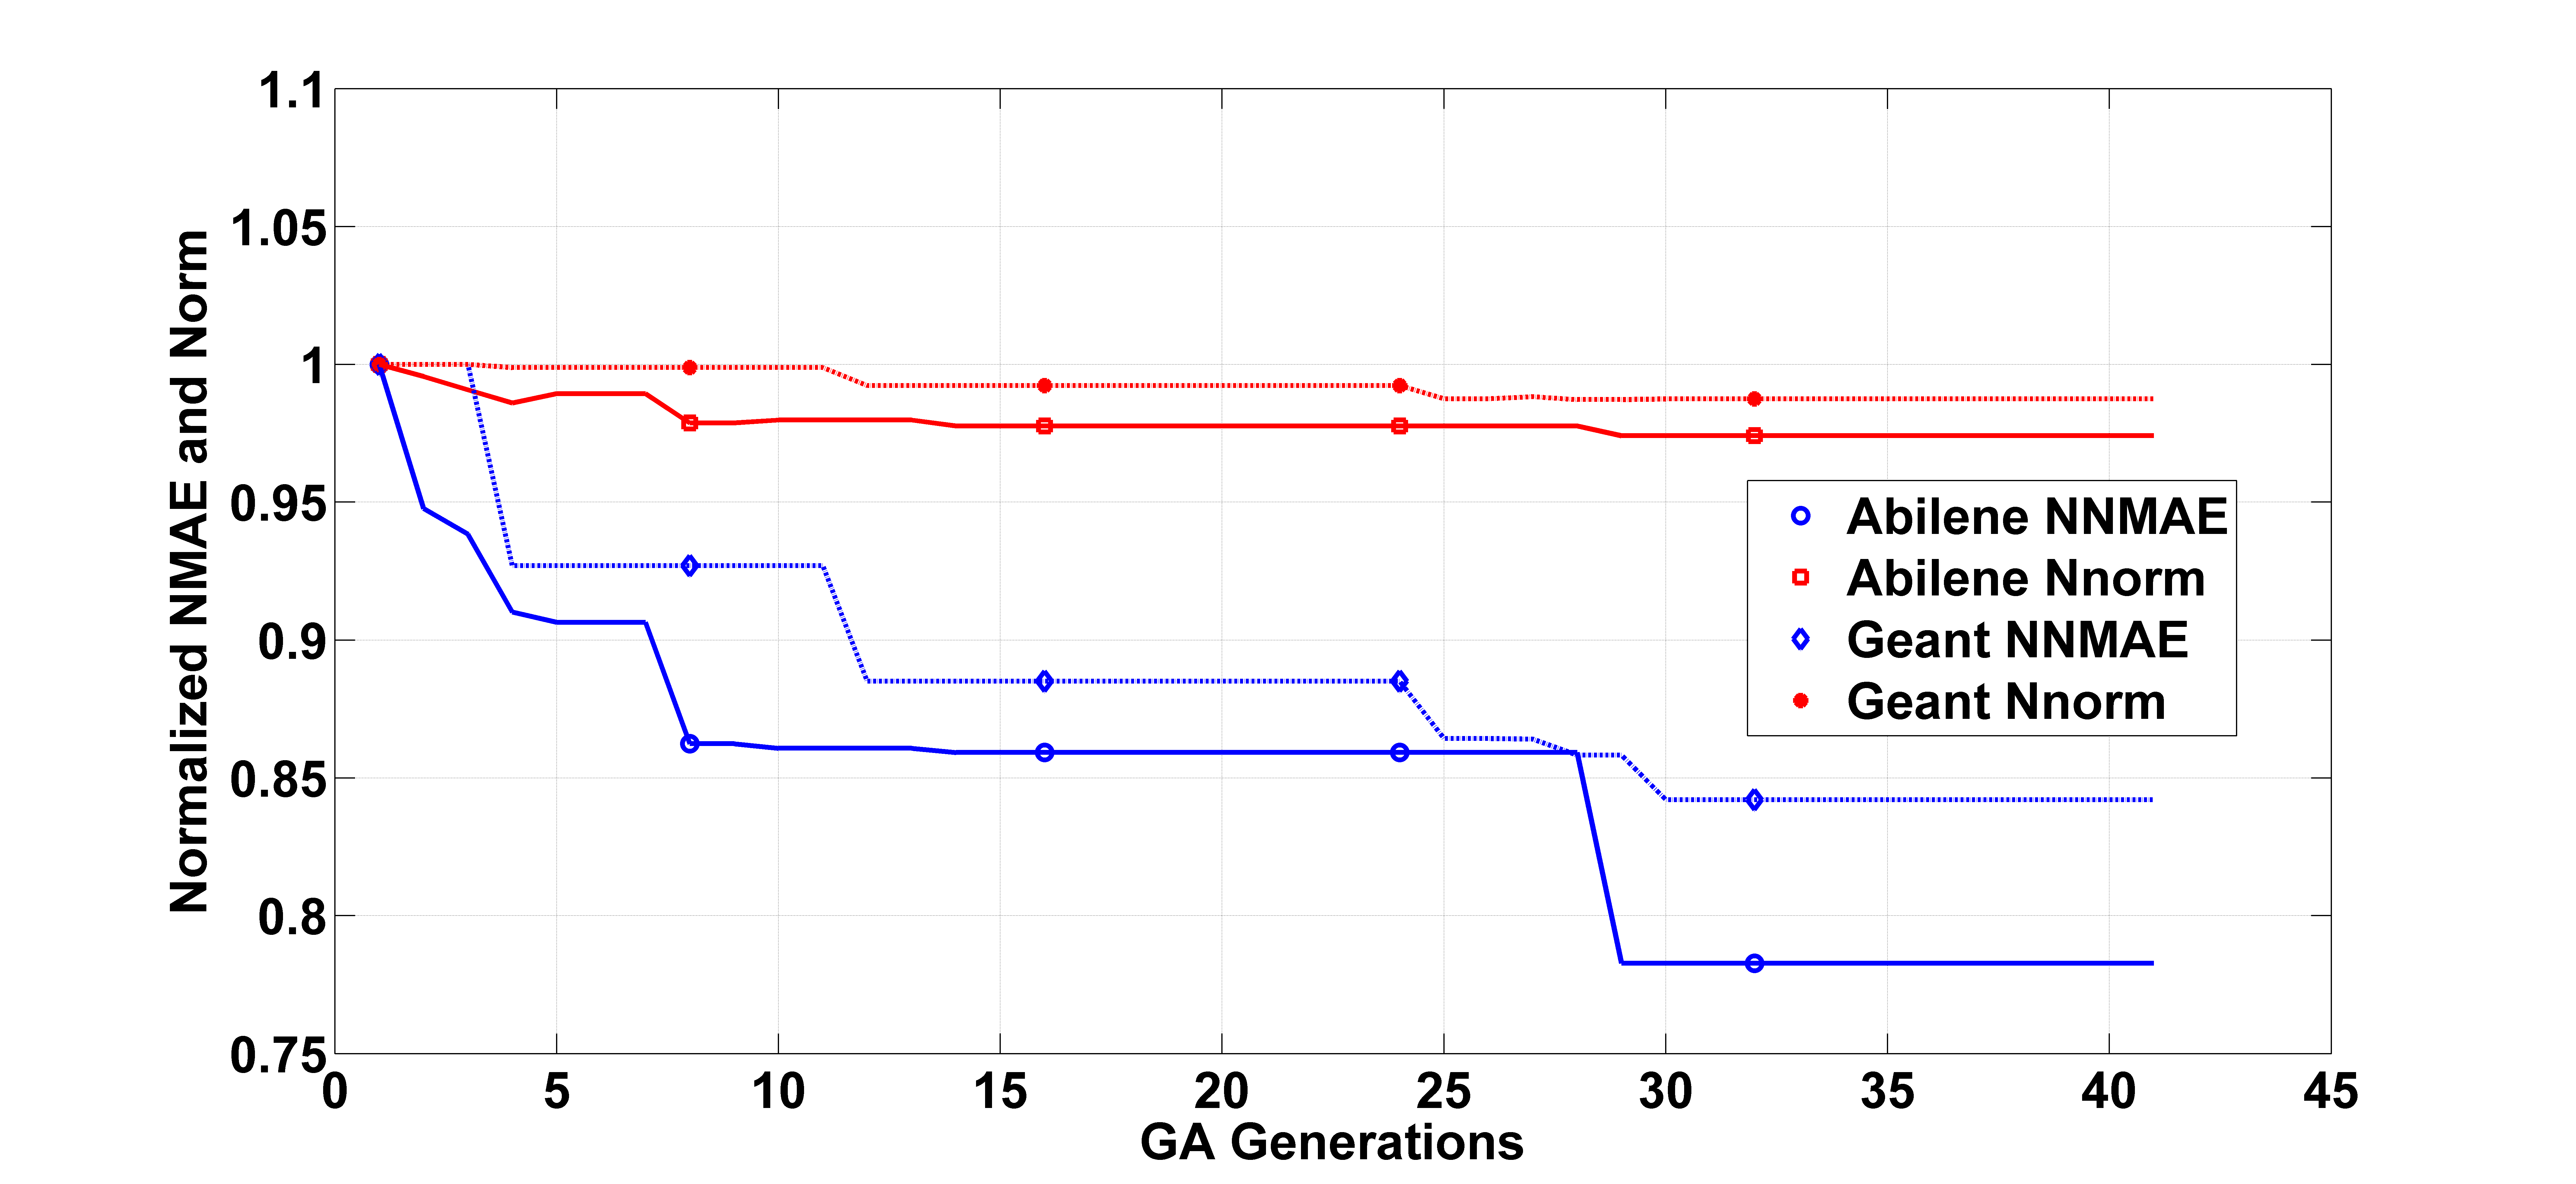
\includegraphics[keepaspectratio, width=0.49\textwidth]{AbileneGeantGAEvolution.png}}
%  \end{center}
%  \caption{{\footnotesize{The evolution of normalized $NMAE$ and norm in the GA.}}}
%  \label{fig:NMAENormCorrFig}
%\end{figure}
%
%\begin{table}
%	\centering
% \small{
% \renewcommand{\tabcolsep}{0.05cm}
% \renewcommand{\arraystretch}{1.0}
%		\begin{tabular}{| c | c | c | c | c |}
%		\hline
%                       & $SR=0.2$ & $SR=0.3$ & $SR=0.4$ & $SR=0.5$   \\ \hline
%      $\rho$ Abilene   & 0.9089 & 0.9640 & 0.7546 & 0.9698 \\ \hline
%      $\rho$ Geant     & 0.9337 & 0.8805 & 0.9617 & 0.8791 \\ \hline
%    \end{tabular}
%	\caption{\scriptsize{Correlation coefficient $\rho:=\frac{Cov(NMAE,\sigma_{1}(\Omega))}{\sqrt{Var(NMAE)Var(\sigma_{1}(\Omega))}}$ between NMAE and the norm of the observation matrix}}
%	\label{tab:NMAENormCorrTab}
%}
%\end{table}

\subsection{Deployability of SNIPER in Dynamic Environments}
In the case of supervised learning, the SNIPER framework computes the optimal sampling matrix using the training data, available in the initial learning stage. The training data-set can be obtained by directly measuring the required IAI in the beginning or by using already available data-sets (e.g. NetFlow records in the case of TM completion). Under hard constraint of network measurement resources, to effectively apply the SNIPER framework in dynamic environments, it is important to: 1) decrease the dependency of the SNIPER framework on the initial training data-set, and 2) adaptively update the OOM designed in the learning stage based on the most current behavior of the network under study. Accordingly, here, we propose a new algorithm that can be effectively utilized for network measurement purposes in the SNIPER framework. 

In this algorithm, first, we determine the initial sampling ratio (indicated by $s_{0}$) and over the initial period we use SDN flexibility to randomly measure a sub-set of IAI to form a matrix with size $n \times T_{0}$. Then, we apply the appropriate matrix completion on this matrix of IAI to estimate unknown IAI and form our new training data-set. Then we apply the evolutionary optimization algorithm (e.g. GA) on this new training data-set to compute the OOM. By applying the MC algorithm using this OOM we can estimate all unknown IAI. Since the largest IAI are potentially the most informative ones for increasing the estimation accuracy (according to the recent study in \cite{IF14iSTAMP:2014}), to adaptively update the OOM for use in the next measurement epoch, we also choose a fraction of largest estimated IAI (indicated by $k_{0}\%$) to be measured directly. That is, after learning epoch where the OOM is designed using the new training data-set, we modify this optimal measurement matrix by adding $k_{0}\%$ of direct measurements which are indicated by the largest estimated IAI in the previous epoch. 

Table \ref{tab:NMAEDGA} shows the performance of this algorithm in flow-size estimation where the genetic algorithm is used to design the OOM. Here, the notions of DGA and DRS are respectively used to denote Dynamic GA and Dynamic RS indicating the case where initial observation matrix is adaptively updated. It is clear that, under hard resource constraint of TCAM entries, that is at low sampling ratio $s$=0.2, DGA is able to provide more accurate estimates for both Abilene and Geant networks. Note that there is a trade-off between performance and parameters $s_{0}$, which controls the dependency of SNIPER framework on training data-set. Moreover, Table \ref{tab:PdPfaDGA} shows the performance of this algorithm for the reliable detection of heavy hitters where the threshold $\theta$ (see Section \ref{sec:SNIPERPerfEvalApp}) varies from $5\%$ to $25\%$ of the largest flow in the data-set. As it was expected, by increasing threshold, $P^{d}_{HH}$ and $P^{fa}_{HH}$ are decreased. However, it provides a reliable detection performance, in all cases, indicating the effectiveness of the adaptive updating of OOM. This indicates the ability of SNIPER for identifying HH which is of great importance in network traffic engineering and network security applications. Note that the performance can be improved by increasing $k_{0}(\%)$ which determines the number of new measurements, updating the OOM matrix.
%The OEOA can be used by the SNIPER framework to improve its performance in dynamic environments where the characteristics of the IAI varies and online measurements are needed to capture the most current behavior of the network under study. Assuming a pre-determined sampling ratio, the OEOA is performed in the following steps.
%
%It starts by the random measurement of a sub-set of the attribute of interests (denoted by $\Omega$). Then, it applies the matrix completion technique to estimate unobserved IAI in the set $\bar{\Omega}$. Next, it considers the estimates in the first step (in the set $\bar{\Omega}$) as measurements and apply the same MC technique to estimate the entries in the set $\Omega$ that we have already measured them, precisely. Now, the OEOA has the ability to evaluate the fitness value for each solution in the population
%
%\begin{table}
	%\centering
%%  \footnotesize{
 %\small{
 %% \renewcommand{\tabcolsep}{0.05cm}
 %% \renewcommand{\arraystretch}{1.0}
		%\begin{tabular}{| c | c | c | c | c | c | c |}
		%\hline
       %$SR$                                  &    $RS_{T_{0}}$  &  $GA_{T_{0}}$  &  $GA_{Avg}$  &  $RS_{Avg}$ &  $DRS_{Avg}$ &  $DGA_{Avg}$ \\ \hline
      %Abilene ($s_{0}$=0.5) &        &       &      &     &  &        \\ \hline
      %Abilene ($s_{0}$=0.6) &        &       &      &     &  &        \\ \hline
      %Abilene ($s_{0}$=0.7) &        &       &      &     &  &        \\ \hline
      %Geant ($s_{0}$=0.5)   &        &       &      &     &  &         \\ \hline
      %Geant ($s_{0}$=0.6)   &        &       &      &     &  &         \\ \hline
      %Geant ($s_{0}$=0.7)   &        &       &      &     &  &         \\ \hline
    %\end{tabular}
	%\caption{\small{$NMAE$ for different $s_{0}$ where $s$=0.2 and $k_{0}=5$.}}
	%\label{tab:NMAEDGA}
%}
%\end{table}

% s_{0} = 0.6 was removed because the new initial data set that is formed is not the same among others
\begin{table}
	\centering
%  \footnotesize{
 %\small{
 % \renewcommand{\tabcolsep}{0.05cm}
 % \renewcommand{\arraystretch}{1.0}
		\begin{tabular}{| c | c | c | c | c |}
		\hline
       $SR$                 &    $DRS_{T_{0}}$  &  $DGA_{T_{0}}$  &  $DRS_{Avg}$ &  $DGA_{Avg}$ \\ \hline
      Abilene ($s_{0}$=1.0) & 0.7100 & 0.5433 & 0.5550 & 0.4696        \\ \hline
      Abilene ($s_{0}$=0.8) & 0.7278 & 0.5779 & 0.5666 & 0.5076        \\ \hline
      % Abilene ($s_{0}$=0.6) & 0.7100 & 0.5683 & 0.5475 & 0.5231        \\ \hline
      Geant ($s_{0}$=1.0)   & 0.7284 & 0.5860 & 0.5474 & 0.5420         \\ \hline
      Geant ($s_{0}$=0.8)   & 0.7311 & 0.5936 & 0.5697 & 0.5567         \\ \hline
      % Geant ($s_{0}$=0.6)   & 0.7024 & 0.6187 & 0.5550 & 0.5280         \\ \hline
    \end{tabular}
		\vspace{0.15cm}
	\caption{{$NMAE$ for different $s_{0}$ where $s$=0.2 and $k_{0}=5\%$.}}
	\label{tab:NMAEDGA}
%}
\end{table}

\begin{table}
	\centering
%  \footnotesize{
 %\small{
 % \renewcommand{\tabcolsep}{0.05cm}
 % \renewcommand{\arraystretch}{1.0}
		\begin{tabular}{| c | c | c | c | c | c |}
		\hline
       $\theta$             &  5\%  &  10\%  &  15\%  & 20\%  & 25\% \\ \hline
      $P^{d}_{HH}$ (Abilen)  & 0.8837 & 0.8559 & 0.8633 & 0.8491 & 0.8252        \\ \hline
      $P^{fa}_{HH}$ (Abilen) & 0.0206 & 0.0115 & 0.0073 & 0.0053 & 0.0042       \\ \hline
      $P^{d}_{HH}$ (Geant)   & 0.9108 & 0.9480 & 0.9662 & 0.9631 & 0.9610        \\ \hline
      $P^{fa}_{HH}$ (Geant)  & 0.0103 & 0.0059 & 0.0043 & 0.0034 & 0.0024        \\ \hline
    \end{tabular}
		\vspace{0.15cm}
	\caption{{$P^{d}_{HH}$ and $P^{fa}_{HH}$ for different $s_{0}$ where $s$=0.2 and $k_{0}=5\%$.}}
	\label{tab:PdPfaDGA}
%}
\end{table}

%The OEOA can be used by the SNIPER framework to improve its performance in dynamic environments where the characteristics of the IAI varies and online measurements are needed to capture the most current behavior of the network under study. Assuming a pre-determined sampling ratio, the OEOA is performed in the following steps.
%
%It starts by the random measurement of a sub-set of the attribute of interests (denoted by $\Omega$). Then, it applies the matrix completion technique to estimate unobserved IAI in the set $\bar{\Omega}$. Next, it considers the estimates in the first step (in the set $\bar{\Omega}$) as measurements and apply the same MC technique to estimate the entries in the set $\Omega$ that we have already measured them, precisely. Now, the OEOA has the ability to evaluate the fitness value for each solution in the population
%
%$$ or NMAE in By evaluating  
%
%
%
%
%Now, we can evaluate the exact 
%
%
%First, , it randomly measures a sub-set of the attribute of interests (denoted by $\Omega$) and apply the matrix completion technique to estimate unobserved IAI in the set $\bar{\Omega}$. Then, it considers the estimates in the first step (in the set $\bar{\Omega}$) as measurements and apply the same MC technique to estimate the entries in the set $\Omega$ that we have already measured them, precisely. Now, we can evaluate the exact 
%
%Under supervised learning, the SNIPER framework is based on  
%
%
%An OLGA differs from standard
%genetic algorithms in that it does not repeatedly evaluate individuals
%against a fixed set of training examples. Instead, it
%is presented with a series of training examples, one at a time,
%and does not retain the entire set for training.
%
%
%By evaluating
%individuals on recent examples, OLGAs also better mimic
%the behavior of natural selection, as real organisms live in environments
%that are not identical to that of their ancestors.
%
%
%In iSTAMP the feasibility of the flow aggregation process is important. In our optimal aggregation matrix design (Eq.(\ref{FAgOpt3})), the feasibility, now considered in feasibility sets $\left\{\mathcal{F}_{i}\right\}_{i=1}^{m}$, can be simply modeled as another linear constraint and our CPLEX engine can efficiently solve it. However, in our abstract flow estimation models (Eq.(\ref{ISDNFMOpt1})-Eq.(\ref{ISDNFMOpt2})), we assume flows can be aggregated without any constraints. In the absence of SNMP link load measurements, BAT is the model used to address this constraint where feasible aggregable flows are grouped together and Eq.(\ref{ISDNFMOpt1}) is solved for flow size estimation. In the presence of SNMP side information, the feasibility constraint of the aggregation now has less impact on the overall estimation performance. In this case, Eq.(\ref{ISDNFMOpt2}) is used to provide fine grained flow estimates and aggregated flow measurements act as side information for this optimization problem to improve the estimation accuracy, as shown in Fig. \ref{fig:GeantNMSEwwoSI}. Tab. \ref{tab:iSTAMPEATRndDev} shows that iSTAMP using EAT is able to provide a good estimation accuracy even when particular percentage of aggregated flows are randomly deviated from optimal exponential aggregation method Alg.\ref{alg:EAG}. Hence, in essence, iSTAMP is flexible enough to cope with different aggregation constraints. 
%% In addition, the de-aggregation process in iSTAMP helps to cope with feasibility constraints. 
%
%
%\begin{table}
%	\centering
% \footnotesize{
% \renewcommand{\tabcolsep}{0.05cm}
% \renewcommand{\arraystretch}{1.0}
%		\begin{tabular}{| c | c | c | c | c |}
%		\hline
%           $SR$    &   0.2     &   0.3    &   0.4   &     0.5  \\ \hline
%      $OGA_{Avg}$  &   0.7583  &  0.4538  &  0.3651 &   0.3369 \\ \hline
%       $GA_{Avg}$  &   0.6178  &  0.4668  &  0.3602 &   0.3241 \\ \hline
%       $RS_{Avg}$  &   0.7479  &  0.5344  &  0.4245 &   0.3974 \\ \hline
%    \end{tabular}
%    \newline
%\vspace*{0.15cm}
%\newline
%		\begin{tabular}{| c | c | c | c | c |}
%		\hline
%           $SR$    &   0.2     &   0.3    &   0.4   &     0.5  \\ \hline
%      $OGA_{Avg}$  &   0.5954  &  0.3839  &  0.2590 &   0.2259 \\ \hline
%       $GA_{Avg}$  &   0.6070  &  0.3757  &  0.2516 &   0.2129 \\ \hline
%       $RS_{Avg}$  &   0.7076  &  0.4683  &  0.3031 &   0.2497 \\ \hline
%    \end{tabular}
%	\caption{\scriptsize{$NMAE$ comparison among $OGA$, $GA$ and $RS$ for Abilene and Geant networks, respectively.}}
%	\label{tab:OnlineGA}
%}
%\end{table}

\subsection{Feasibility of SNIPER} 
To show the feasibility of the SNIPER, we have implemented a prototype of the SNIPER for per-flow size estimation in Mininet which is a network testbed for developing OpenFlow and SDN experiments \cite{MininetOrg}. We implement the SNIPER controller in POX and, also, we emulate the Geant network and feed it with real traffic traces (see Table \ref{tab:DataSetProp}). Table \ref{tab:SNIPERGeantMininetRes} summarizes the results of our implementation of the SNIPER framework in Mininet, demonstrating the feasibility of the implementation of the SNIPER framework in production environments. Here, the optimal sampling matrix is designed using genetic algorithm for different sampling ratios and, it is clear that the OOM designed by the GA can obtain a better estimation accuracy.

%\begin{table}
%	\centering
% \footnotesize{
% \renewcommand{\tabcolsep}{0.05cm}
% \renewcommand{\arraystretch}{1.0}
%		\begin{tabular}{| c | c | c | c | c |}
%		\hline
%                  & $GA_{T_{0}}$  &  $RS_{T_{0}}$  &  $GA_{{Avg}}$  &  $RS_{{Avg}}$  \\ \hline
%      $SR$=0.2    & 0.7734        & 0.8354         & 0.7946         & 0.8612	     \\ \hline
%      $SR$=0.3    & 0.6646        & 0.6667	       & 0.6422	        & 0.6587	     \\ \hline
%    \end{tabular}
%	\caption{\scriptsize{The $NMAE$ via implementing SNIPER for Geant Network in Mininet at different $SR$s.}}
%	\label{tab:SNIPERGeantMininetRes}
%}
%\end{table}
\begin{table}
	\centering
 %\small{
 % \renewcommand{\tabcolsep}{0.05cm}
 % \renewcommand{\arraystretch}{1.0}
		\begin{tabular}{| c | c | c | c | c |}
		\hline
       $SR$           & 0.2    &  0.3    &  0.4    &  0.5  \\ \hline
      $GA_{T_{0}}$    & 0.7739 &	0.6646 &	0.5380 &	0.4341     \\ \hline
      $RS_{T_{0}}$    & 0.8354 &	0.6667 &	0.5561 &	0.4518     \\ \hline
      $GA_{{Avg}}$    & 0.7946 &	0.6422 & 	0.5172 &	0.4272     \\ \hline
      $RS_{{Avg}}$    & 0.8612 &	0.6587 &	0.5323 &	0.4377     \\ \hline
    \end{tabular}
		\vspace{0.15cm}
	\caption{{$NMAE$ via implementing SNIPER for Geant network in Mininet.}}
	\label{tab:SNIPERGeantMininetRes}
%}
\end{table}

% We create two networks that emulates Geant and Data Center environments and feed these two networks with real traffic traces listed in Tab. \ref{tab:DataSetProp}. Tab. \ref{tab:MininetResultsTab1} summarizes the results of our implementation in Mininet, demonstrating the effectiveness and feasibility of iSTAMP in production environments. Geant(1) and Data Center denote single point measurement scenario and Geant(2) denotes multi-point measurement scheme involving multiple Capableness routers running iSTAMP framework. 







%% P^{d} is P11 and P^{fa} is P01 shayad behtar ast dar figure gozashte shavad
%\begin{table}
%	\centering
% \small{
% \renewcommand{\tabcolsep}{0.05cm}
% \renewcommand{\arraystretch}{1.0}
%		\begin{tabular}{| c | c | c | c | c | c | c | c | c | c |}
%		\hline
%                                   & $SR=0.01$ & and continue for all SR values   \\ \hline
%      $P^{d}_{CP}$ Abilene  (RS)   & & ... \\ \hline
%      $P^{d}_{CP}$ Abilene  (GA)   & & ... \\ \hline
%      $P^{d}_{CP}$ Abilene  (PSO)   & & ... \\ \hline
%      $P^{fa}_{CP}$ Abilene   (RS) & & ... \\ \hline
%      $P^{fa}_{CP}$ Abilene   (GA) & & ... \\ \hline
%      $P^{fa}_{CP}$ Abilene   (PSO) & & ... \\ \hline
%    \end{tabular}
%	\caption{\scriptsize{Comparing the average $P^{d}_{HH}$ and $P^{fa}_{HH}$ between RS, GA and PSO sampling methods for Harvard network.}}
%	\label{tab:SNIPERPdPfaHH}
%}
%\end{table}
%As we have seen in the previous results, the SNIPER can improve the estimation accuracy under hard constraints of measurement resources. However, since the genetic algorithm targets the ultimate matrix completion inference performance, the processing power is problematic in large-scale networks and this limits the scalability of the SNIPER framework. To reduce the computational complexity and processing power of the SNIPER two approaches are considered here. First, instead of minimizing the ultimate estimation accuracy (e.g. represented by $NMAE$), the norm of the observation matrix $\Omega$ is minimized where the norm of a matrix is defined as the maximum singular value of the matrix. Note that, the norm of the observation matrix is strongly correlated with $NMAE$; this fact has been justified in Figure \ref{fig:NMAENormCorrFig} and Table \ref{tab:NMAENormCorrTab}. Second, instead of using the GA we use the PSO evolutionary optimization algorithm which is much faster than the GA and can reduce the computational complexity of the SNIPER and accordingly, reduce the processing power.





%%%% % \section{Some Tables}


$SR$ denotes the Sampling Ratio.

\begin{table}
	\centering
 \footnotesize{
 \renewcommand{\tabcolsep}{0.05cm}
 \renewcommand{\arraystretch}{1.0}
		\begin{tabular}{| c | c | c | c | c | c | c | c |}
		\hline
       Net./Prm. & $SR$ & $RS_{T_{0}}$ & $GA_{T_{0}}$ & $PSO_{T_{0}}$ & $RS^{\sigma}_{T_{0}}$ & $GA^{\sigma}_{T_{0}}$ & $PSO^{\sigma}_{T_{0}}$  \\ \hline
      Abilene    & 0.3 & 0.499312 & 0.364073 & 0.387655 & 0.498732 & 0.503375 & 0.480801 \\ \hline
      GEANT      & 0.2 & 0.728394 & 0.55408 & 0.60432 & 0.722275 & 0.679437 & 0.684696 \\ \hline
    \end{tabular}
    \newline
\vspace*{0.15cm}
\newline
		\begin{tabular}{| c | c | c | c | c | c | c | c |}
		\hline
       Net./Prm. & $SR$ & $RS_{Avg}$ & $GA_{Avg}$ & $PSO_{Avg}$ & $RS^{\sigma}_{Avg}$ & $GA^{\sigma}_{Avg}$ & $PSO^{\sigma}_{Avg}$  \\ \hline
      Abilene    & 0.3 & 0.569638 & 0.556108 & 0.494916 & 0.582961 & 0.546438 & 0.586098  \\ \hline
      GEANT      & 0.2 & 0.686854 & 0.601478 & 0.644993 & 0.69442 & 0.664646 & 0.681144  \\ \hline
    \end{tabular}
	\caption{\scriptsize{NMAE comparison between different evolutionary fitness functions ($\sigma$ denotes norm function).}}
	\label{tab:FitFuncCmp1}
}
\end{table}



\begin{table}
	\centering
 \footnotesize{
 \renewcommand{\tabcolsep}{0.05cm}
 \renewcommand{\arraystretch}{1.0}
		\begin{tabular}{| c | c | c | c | c | c | c | c |}
		\hline
       Net./Prm. & $SR$ & $RS_{T_{0}}$ & $GA_{T_{0}}$ & $PSO_{T_{0}}$ & $RS^{\mu}_{T_{0}}$ & $GA^{\mu}_{T_{0}}$ & $PSO^{\mu}_{T_{0}}$  \\ \hline
      Abilene    & 0.3 & 0.499312 & 0.364073 & 0.387655 & 0.498444 & 0.586809 & 0.506632 \\ \hline
      GEANT      & 0.2 & 0.728394 & 0.55408 & 0.60432 & 0.726252 & 0.671924 & 0.701205 \\ \hline
    \end{tabular}
    \newline
\vspace*{0.15cm}
\newline
		\begin{tabular}{| c | c | c | c | c | c | c | c |}
		\hline
       Net./Prm. & $SR$ & $RS_{Avg}$ & $GA_{Avg}$ & $PSO_{Avg}$ & $RS^{\mu}_{Avg}$ & $GA^{\mu}_{Avg}$ & $PSO^{\mu}_{Avg}$  \\ \hline
      Abilene    & 0.3 & 0.569638 & 0.556108 & 0.494916 & 0.553764 & 0.602730 & 0.517396  \\ \hline
      GEANT      & 0.2 & 0.686854 & 0.601478 & 0.644993 & 0.719503 & 0.662732 & 0.752084  \\ \hline
    \end{tabular}
	\caption{\scriptsize{NMAE comparison between different evolutionary fitness functions ($\mu$ denotes average coherence function).}}
	\label{tab:FitFuncCmp1}
}
\end{table}


\begin{table}
	\centering
 \footnotesize{
 \renewcommand{\tabcolsep}{0.05cm}
 \renewcommand{\arraystretch}{1.0}
		\begin{tabular}{| c | c | c | c |}
		\hline
       Net./TimeGain & $SR$ & $Time Gain^{\sigma}_{GA}$ & $Time Gain^{sigma}_{PSO}$ \\ \hline
      Abilene    & 0.3 & 0.937689 & 0.818912  \\ \hline
      GEANT      & 0.2 & 0.884593 & 0.773611  \\ \hline
    \end{tabular}
	\caption{\scriptsize{Time Gain comparison between different evolutionary fitness functions ($\sigma$ denotes norm function).}}
	\label{tab:FitFuncCmp2}
}
\end{table}


\begin{table}
	\centering
 \footnotesize{
 \renewcommand{\tabcolsep}{0.05cm}
 \renewcommand{\arraystretch}{1.0}
		\begin{tabular}{| c | c | c | c |}
		\hline
       Net./TimeGain & $SR$ & $Time Gain^{\mu}_{GA}$ & $Time Gain^{\mu}_{PSO}$ \\ \hline
      Abilene    & 0.3 & 0.860323 & 0.663545  \\ \hline
      GEANT      & 0.2 & 0.815136 & 0.698976  \\ \hline
    \end{tabular}
	\caption{\scriptsize{Time Gain comparison between different evolutionary fitness functions ($\mu$ denotes average coherence function).}}
	\label{tab:FitFuncCmp2}
}
\end{table}


%
\section{Discussion and Conclusion}  \label{sec:Conclu}
%Comparing with the state of the art SDN frameworks in \cite{IF14iSTAMP:2014} and \cite{Adrichen:2014} that have been used for \emph{fine-grained} network performance measurements, SNIPER can be used in a wide range of network monitoring applications under hard network resource constraints while, it is still capable of providing estimates of IAI with acceptable accuracy and reliability, based on the application. The computational complexity and communication overhead of the SNIPER frame work are low while it does not suffer from feasibility constraints as in \cite{IF14iSTAMP:2014}. Such capabilities are based on the fact that: 1) the SNIPER is a SDN measurement framework; 2) the main NI technique in SNIPER is the matrix completion algorithm, where providing the required measurement of IAI is feasible, and 3) the OOM required by matrix completion techniques is designed using EOAs to provide the most informative measurements with the smallest amount of resources. We showed that SNIPER is a generic, flexible and efficient framework that can be used for a variety of network monitoring applications under hard resource constraints.
Table \ref{tab:SDNFrmCmp} compares the performance of SNIPER with the state of the art SDN frameworks in \cite{IF14iSTAMP:2014} and \cite{Adrichen:2014} that have been used for \emph{fine-grained} network performance measurements. The comparison in this table is qualitative because the exact comparison between SNIPER and these two frameworks is difficult due to the facts that: 1) the traffic matrix estimation techniques and criterion in \cite{IF14iSTAMP:2014} are different from SNIPER, and 2) in \cite{Adrichen:2014}, the IAI are directly measured for different network(s) where the same data-sets are unavailable.

This table shows that there is a tradeoff between different parameters that must be considered in the design of effective network measurement systems. Among these, SNIPER can be used in a wide range of network monitoring applications under hard network resource constraints while, it is still capable of providing estimates of IAI with acceptable accuracy and reliability, based on the application. The computation and communication overhead of the SNIPER frame work are low while it does not suffer from feasibility constraints as in \cite{IF14iSTAMP:2014}. Such capabilities are based on the fact that: 1) the SNIPER is a SDN measurement framework with high flexibility; 2) the main NI technique in SNIPER is matrix completion algorithm, where providing the required independent measurements of IAI is feasible, and 3) the OOM required by MC techniques is designed using EOAs to provide the most informative measurements with the smallest amount of resources. We showed the effectiveness of SNIPER in different network monitoring applications and under hard resource constraints.

\begin{table}
\centering
	{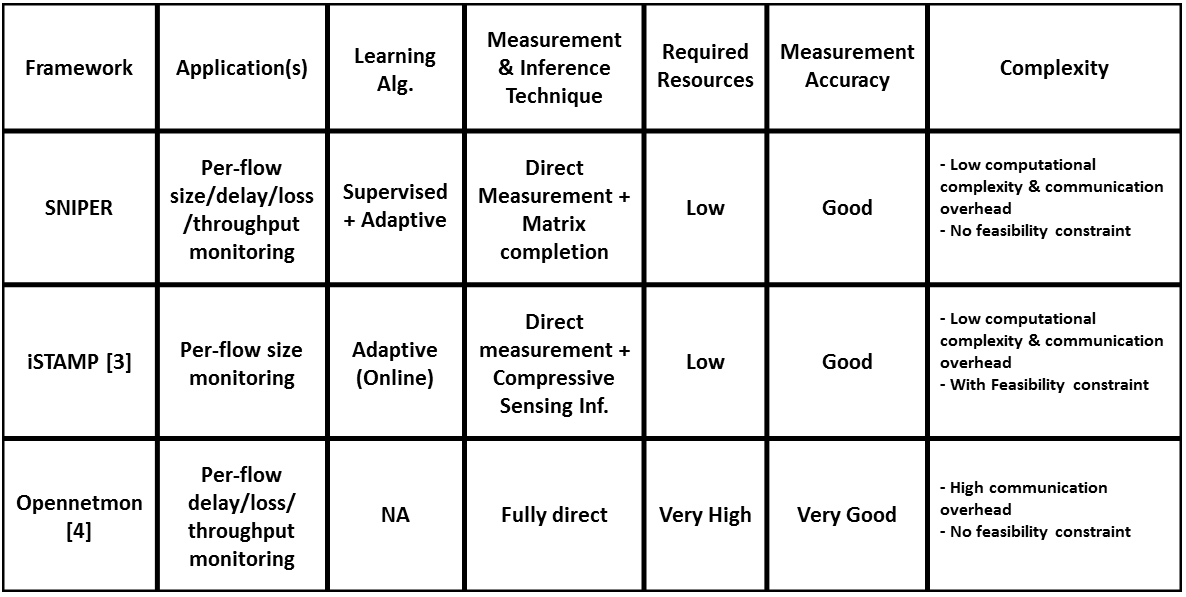
\includegraphics[keepaspectratio, width=0.42\textwidth]{CompTable_New2.png}} 
  % \includegraphics[width=\linewidth]{excel-table}
  \caption{{A comparison between SDN network measurement frameworks.}}
  \label{tab:SDNFrmCmp}
\end{table}


%In this paper we introduced SNIPER, an intelligent network measurement framework, where the flexibility provided by SDN is used to optimally design the observation or measurement matrix which leads to the best possible estimation accuracy via applying matrix completion techniques. 
%Since the design of optimal binary observation matrices using integer optimization techniques is extremely complicated and computationally expensive, here, we have formulated this problem using evolutionary optimization algorithms including genetic algorithm and particle swarm optimization algorithm. We have shown that both methods can be used by the SNIPER framework to effectively design the optimal measurement matrices under hard constraint of measurement resources. The effectiveness of this method have been examined using both synthetic and real network measurement traces from different network topologies and by considering two main applications including network traffic and delay estimations. The feasibility of our framework has also verified by implementing a prototype of SNIPER in Mininet environment.
%In this paper we introduced SNIPER, an intelligent network measurement framework, where the flexibility provided by SDN is used to optimally design the observation or measurement matrix which leads to the best possible estimation accuracy via applying matrix completion techniques. 
%Since the design of optimal binary observation matrices using integer optimization techniques is extremely complicated and computationally expensive, here, we have formulated this problem using evolutionary optimization algorithms including genetic algorithm and particle swarm optimization algorithm. We have shown that both methods can be used by the SNIPER framework to effectively design the optimal measurement matrices under hard constraint of measurement resources. The effectiveness of this method have been examined using both synthetic and real network measurement traces from different network topologies and by considering two main applications including network traffic and delay estimations. The feasibility of our framework has also verified by implementing a prototype of SNIPER in Mininet environment.
% SNIPER in recommended systems by intelligent and active interaction with the system to sample the best points


%\begin{table}
	%\centering
%%  \footnotesize{
 %\small{
 %% \renewcommand{\tabcolsep}{0.05cm}
 %% \renewcommand{\arraystretch}{1.0}
		%\begin{tabular}{| c | c | c | c | c | c | c | c |}
		%\hline
       %Framework &    \\ \hline
    %\end{tabular}
	%\caption{\scriptsize{The average of $P^{d}_{CP}$ and $P^{fa}_{CP}$ for Harvard network in different sampling ratios.}}
	%\label{tab:PdfaHarvard}
%}
%\end{table}

%%% \section{Acknowledgements}
This work is supported by NSF CNS-1321115 grant and HP Labs Innovation Research Award.

\bibliographystyle{ieeetr}
\bibliography{SNIPER14_Bib}

%\bibliographystyle{abbrv}
%\bibliography{SNIPER14_Bib}


%% \onecolumn
%\input{IF14_AppA}
%% \input{IF14_AppB}

\end{document}